% =====================================================================
% PLANTILLA DEL SEGUNDO TALLER
% Mecanismos de Seguridad
% Facultad de Ingeniería
% Universidad Distrital Francisco José de Caldas
%
% Estructura del proyecto:
%   main.tex                 Preámbulo, portada y ensamblado del documento
%   referencias.bib          Fuentes en BibLaTeX (estilo APA 7)
%   imagenes/                Logo institucional y figuras
%   secciones/               Contenido dividido por secciones
%     secciones/03-casos/    Una ficha independiente por caso (10 casos)
%
% Compilación recomendada:
%   latexmk -pdf main.tex
%
% Si se compila manualmente:
%   pdflatex main.tex
%   biber main
%   pdflatex main.tex
%   pdflatex main.tex
% =====================================================================

\documentclass[stu, 12pt, letterpaper, donotrepeattitle, floatsintext]{apa7}

% ---------------------------------------------------------------------
% Paquetes generales
% ---------------------------------------------------------------------
\usepackage[T1]{fontenc}
\usepackage[utf8]{inputenc}
\usepackage[spanish,es-noquoting]{babel}
\usepackage{csquotes}
\usepackage{newtxtext,newtxmath}
\usepackage{graphicx}
\graphicspath{{imagenes/}}
\usepackage{array}
\usepackage{booktabs}
\usepackage{longtable}
\usepackage{makecell}
\usepackage{tabularx}
\usepackage{setspace}
\usepackage{ragged2e}
\usepackage{float}
\usepackage{enumitem}
\usepackage{xcolor}
\usepackage{colortbl}
\usepackage{pdflscape}
\usepackage[most]{tcolorbox}
\usepackage[style=apa, backend=biber]{biblatex}
\DeclareLanguageMapping{spanish}{spanish-apa}
\addbibresource{referencias.bib}
\AtBeginBibliography{\justifying\sloppy}
\hypersetup{hidelinks}

% ---------------------------------------------------------------------
% Justificación robusta
% Las líneas con comandos \texttt largos (nmap, tshark, rutas) tienen
% pocos puntos donde partirse. Sin holgura adicional, TeX comprime la
% glue interpalabra hasta cero y las palabras quedan pegadas. Con
% emergencystretch solo se relajan las líneas que de otro modo
% desbordarían el margen.
% ---------------------------------------------------------------------
\usepackage{microtype}
% Deben fijarse al comenzar el documento: las asignaciones hechas en el
% preámbulo quedan dentro del grupo que LaTeX cierra en \begin{document}.
\AtBeginDocument{%
	\setlength{\emergencystretch}{3em}%
	\tolerance=9999
	\pretolerance=-1
	\hbadness=10000
}
% Algunas cajas y entornos restauran \tolerance a 200. Reafirmarlo al
% inicio de cada párrafo garantiza que las líneas con \texttt largos
% puedan optar por una línea holgada en lugar de desbordar el margen.
\AddToHook{para/begin}{\tolerance=9999 \emergencystretch=3em \pretolerance=-1\relax}

% ---------------------------------------------------------------------
% Ajustes de formato
% ---------------------------------------------------------------------
\newcolumntype{Y}{>{\raggedright\arraybackslash}X}

% Casilla vacía para listas de verificación (sin depender de amssymb).
% El \fboxsep se reduce para que la casilla quede cuadrada y discreta.
\newcommand{\checkbox}{{\setlength{\fboxsep}{1pt}\framebox[6pt]{\rule{0pt}{4pt}}}}

% Numeración de secciones y subsecciones: "1", "1.1", "1.2", ...
\setcounter{secnumdepth}{2}

\setlength{\JustifyingParindent}{0.5in}

% "s. f." con espacio, como lo prefiere el estilo APA en español.
\DefineBibliographyStrings{spanish}{%
	nodate = {s.~f\adddot},
}

\AtBeginDocument{%
	\renewcommand{\keywordname}{Palabras clave}%
	\renewcommand{\notelabel}{Nota}%
	\renewcommand{\tablename}{Tabla}%
}

% ---------------------------------------------------------------------
% Cajas de apoyo
% ---------------------------------------------------------------------
\newtcolorbox{situacion}{
	colback=gray!5,
	colframe=gray!55,
	boxrule=0.5pt,
	arc=1.5pt,
	left=6pt,
	right=6pt,
	top=4pt,
	bottom=4pt,
	breakable,
	title={Situación},
	fonttitle=\bfseries,
	coltitle=black
}

\newtcolorbox{nota}[1]{
	colback=blue!3,
	colframe=blue!45!black,
	boxrule=0.5pt,
	arc=1.5pt,
	left=6pt,
	right=6pt,
	top=4pt,
	bottom=4pt,
	title={#1},
	fonttitle=\bfseries,
	coltitle=white
}

% ---------------------------------------------------------------------
% Ficha de registro reutilizable para los diez casos
% ---------------------------------------------------------------------
\newcommand{\registrohallazgo}[1]{%
	\begin{table}[H]
		\centering
		\caption{Ficha de registro del hallazgo. #1}
		\footnotesize
		\renewcommand{\arraystretch}{1.15}
		\begin{tabularx}{\textwidth}{@{}>{\raggedright\arraybackslash}p{0.23\textwidth} Y@{}}
			\toprule
			\textbf{Campo} & \textbf{Registro} \\
			\midrule
			Identificador & \rule{0pt}{0.7cm} \\
			Fecha y hora & \rule{0pt}{0.7cm} \\
			Origen/destino & \rule{0pt}{0.7cm} \\
			Observación & \rule{0pt}{1.5cm} \\
			Hipótesis & \rule{0pt}{1.5cm} \\
			Validación & \rule{0pt}{1.5cm} \\
			Severidad & \rule{0pt}{1.2cm} \\
			Acción & \rule{0pt}{1.5cm} \\
			Integridad & \rule{0pt}{1.0cm} \\
			\bottomrule
		\end{tabularx}
	\end{table}
}

% ---------------------------------------------------------------------
% Metadatos de la portada
% Reemplace los marcadores por los datos reales de los cuatro integrantes.
% No se incluye línea de profesor.
% ---------------------------------------------------------------------
\shorttitle{Segundo Taller de Mecanismos de Seguridad}

\title{%
	
\includegraphics[width=1.9in]{Logo_UD.png}\\[0.6cm]
	Segundo Taller\\[0.15cm]
	Mecanismos de seguridad Informática%
}

\authorsnames{Juan David Orduz Sastoque (20221020096), Jhojan Aragon Ramirez (20221020060), Yader Ibraldo Quiroga Torres (20222020034), Arlo Nicolas Ocampo Gallego (20221020104)}

\authorsaffiliations{{Ingeniería de Sistemas, Facultad de Ingeniería\\Universidad Distrital Francisco José de Caldas}}

\course{Mecanismos de Seguridad}

% Línea de profesor vacía: el taller no solicita nombre del docente.
% \mbox{} evita el error "There's no line here to end" de la clase apa7.
\professor{\mbox{}}

\duedate{14 de noviembre de 2026\\Bogotá, D.C.}

\authornote{Trabajo académico desarrollado en un laboratorio aislado y autorizado. Las pruebas se realizan con equipos propios o máquinas virtuales, direcciones privadas y tráfico de prueba; no se genera tráfico hacia Internet, redes institucionales en producción ni direcciones de terceros.}

% ---------------------------------------------------------------------
% La portada necesita algo menos de aire en el encabezado para que la
% Nota del Autor quepa en la página 1. Se reduce solo el espacio inicial
% que la clase apa7 reserva antes del título (4 -> 2 líneas base).
% ---------------------------------------------------------------------
\usepackage{etoolbox}
\makeatletter
\patchcmd{\maketitle}{\vspace*{4\baselineskip}}{\vspace*{2\baselineskip}}{}{%
	\ClassWarning{apa7}{No se pudo reducir el espacio superior de la portada}}
\makeatother

% =====================================================================
\begin{document}
\maketitle
\tableofcontents
\newpage
\justifying

% ---------------------------------------------------------------------
% Introducción y datos del equipo
% ---------------------------------------------------------------------
\section*{Introducción}
\addcontentsline{toc}{section}{Introducción}

Este documento es la plantilla de trabajo del \textbf{Segundo Taller de Mecanismos de Seguridad}. Reúne, en un solo informe técnico, el análisis de diez casos de seguridad en redes IEEE 802.3 con servicios TCP/IP y el diseño de una solución de programación para el rastreo autorizado de ubicaciones. El taller se desarrolla en un laboratorio académico aislado, con equipos propios o máquinas virtuales, direcciones privadas y tráfico de prueba.

La plantilla está dividida en archivos independientes para facilitar el trabajo en equipo, la revisión por pares y el control de versiones. Cada integrante puede trabajar en su archivo sin sobrescribir el de sus compañeros; al final, todos los archivos se ensamblan en \texttt{main.tex}.

\begin{table}[H]
	\caption{Organización de la plantilla}
	\label{tab:organizacion}
	\centering
	\footnotesize
	\renewcommand{\arraystretch}{1.15}
	\begin{tabularx}{\textwidth}{@{}>{\raggedright\arraybackslash}p{0.38\textwidth} Y@{}}
		\toprule
		\textbf{Archivo} & \textbf{Contenido} \\
		\midrule
		\texttt{main.tex} & Preámbulo, portada, metadatos y ensamblado del documento. \\
		\path{secciones/01-introduccion.tex} & Introducción, alcance, nota ética y datos del equipo. \\
		\path{secciones/02-marco-parte1.tex} & Presentación, objetivos, resultados de aprendizaje, topología, reglas y herramientas. \\
		\path{secciones/03-casos/} & Diez fichas de caso, una por archivo. \\
		\path{secciones/04-registro-hallazgos.tex} & Formato mínimo de registro y consolidado de hallazgos. \\
		\path{secciones/05-entregables-parte1.tex} & Entregables y lista de verificación de la Parte I. \\
		\path{secciones/06-parte2-descripcion.tex} & Descripción y alcance de la solución de rastreo. \\
		\path{secciones/07-parte2-requisitos.tex} & Requisitos funcionales, técnicos y de seguridad. \\
		\path{secciones/08-parte2-arquitectura.tex} & Arquitectura de referencia, modelo de datos y plan de trabajo. \\
		\path{secciones/09-parte2-etica.tex} & Consideraciones éticas, legales y de privacidad. \\
		\path{secciones/10-conclusiones.tex} & Conclusiones y recomendaciones. \\
		\path{secciones/11-anexos.tex} & Registro de evidencias, lista de entrega y glosario. \\
		\texttt{referencias.bib} & Fuentes bibliográficas en formato BibLaTeX (APA 7). \\
		\bottomrule
	\end{tabularx}
\end{table}

\subsection*{Cómo usar la plantilla}

\begin{itemize}[leftmargin=*, topsep=2pt, itemsep=2pt]
	\item Reemplace los marcadores \texttt{Integrante 1}, \texttt{Integrante 2}, \texttt{Integrante 3} e \texttt{Integrante 4} de la portada por los nombres y códigos reales.
	\item Complete la Tabla~\ref{tab:integrantes} con los datos del equipo y la distribución de responsabilidades.
	\item Desarrolle cada caso en su archivo correspondiente. No elimine las preguntas de análisis: responda cada una con evidencia.
	\item Adjunte capturas de pantalla legibles, filtros de Wireshark, extractos de registros y, cuando aplique, el archivo PCAP de laboratorio.
	\item Calcule el hash SHA-256 de cada evidencia original y regístrelo en la ficha del caso y en el Anexo~A.
	\item Verifique que todas las direcciones, nombres y credenciales estén anonimizados antes de entregar el informe.
	\item Cierre el documento con las conclusiones, las limitaciones de la evidencia y las referencias consultadas.
\end{itemize}

\begin{nota}{Alcance ético y legal}
Este taller es un ejercicio académico. No se solicita vulnerar, atacar ni hackear sistemas, redes o personas reales. Todas las actividades de análisis se realizan sobre capturas didácticas, telemetría sintética o pruebas benignas autorizadas en un entorno aislado. El rastreo de ubicaciones de la Parte~II debe operar únicamente con consentimiento informado, finalidad académica y datos anonimizados; no se permite rastrear personas sin autorización ni reutilizar la información para fines distintos de los del taller.
\end{nota}

\subsection*{Datos del equipo}

\begin{table}[H]
	\caption{Integrantes del equipo y distribución de responsabilidades}
	\label{tab:integrantes}
	\centering
	\footnotesize
	\renewcommand{\arraystretch}{1.35}
	\begin{tabularx}{\textwidth}{@{}c >{\raggedright\arraybackslash}p{0.27\textwidth} c Y@{}}
		\toprule
		\textbf{No.} & \textbf{Nombre completo} & \textbf{Código} & \textbf{Responsabilidad principal} \\
		\midrule
		1 & & & \\
		2 & & & \\
		3 & & & \\
		4 & & & \\
		\bottomrule
	\end{tabularx}
\end{table}

\noindent\textbf{Distribución sugerida.} Una distribución equilibrada consiste en asignar los casos 1 a 3 al Integrante~1; los casos 4 y 5, junto con el backend de la Parte~II, al Integrante~2; los casos 6 a 8 y la aplicación móvil al Integrante~3; y los casos 9 y 10, junto con el bot de Telegram y la integración, al Integrante~4. Todos los integrantes deben revisar la versión final y firmar la lista de verificación del Anexo~B.


% ---------------------------------------------------------------------
% PARTE I. ANÁLISIS DE CASOS
% ---------------------------------------------------------------------
\section*{Parte I. Análisis de casos}
\addcontentsline{toc}{section}{Parte I. Análisis de casos}

\section{Presentación y alcance}

La práctica estudia riesgos de disponibilidad, confidencialidad e integridad en una LAN Ethernet IEEE 802.3 que transporta IPv4/IPv6 y servicios TCP/IP. El trabajo se realiza exclusivamente en equipos propios o máquinas virtuales, con direcciones privadas, tráfico de prueba y autorización expresa. No se debe generar tráfico hacia Internet, redes institucionales en producción ni direcciones de terceros.

El alcance del informe comprende el análisis de diez casos críticos, la propuesta de controles preventivos, detectivos, correctivos y de recuperación, y el diseño de una solución de programación para el rastreo autorizado de ubicaciones. Los controles se contrastan con las recomendaciones para sistemas de detección y prevención de intrusiones \parencite{nist80094} y para el endurecimiento de servidores \parencite{nist800123}. Cada afirmación técnica debe sostenerse en evidencia verificable: capturas, registros, filtros, comandos, hashes y marcas de tiempo.

\section{Objetivos}

\begin{itemize}[leftmargin=*, topsep=2pt, itemsep=2pt]
	\item Reconocer indicadores de compromiso y comportamientos anómalos en tráfico TCP, UDP, ICMP, DNS, HTTP/HTTPS y mensajería.
	\item Usar Wireshark y registros del sistema para correlacionar eventos, direcciones, puertos, marcas de tiempo y estados de conexión.
	\item Evaluar controles preventivos y detectivos: firewall, segmentación, endurecimiento de servicios, TLS, limitación de tasa e IDS/SIEM.
	\item Proponer el uso responsable de aprendizaje automático para priorizar alertas, sin delegar bloqueos automáticos críticos a un modelo no validado.
	\item Documentar resultados reproducibles mediante capturas, filtros, registros, hashes y recomendaciones verificables.
	\item Diseñar, en la Parte~II, una propuesta técnica y ética de una aplicación, programa o bot que permita compartir y visualizar ubicaciones con consentimiento informado.
\end{itemize}

\section{Resultados de aprendizaje}

\begin{itemize}[leftmargin=*, topsep=2pt, itemsep=2pt]
	\item Diferencia entre síntoma, indicador, hipótesis y evidencia confirmada.
	\item Interpreta capturas de paquetes y registros sin confundir anomalías con prueba definitiva de ataque.
	\item Relaciona cada caso con controles preventivos, detectivos, correctivos y de recuperación.
	\item Entrega un informe técnico con hallazgos, limitaciones y un plan de mejora priorizado.
\end{itemize}

\section{Topología y reglas del laboratorio}

La topología sugerida es un ejemplo; se pueden usar direcciones privadas equivalentes, siempre que la red permanezca aislada y bajo control del equipo.

\begin{table}[H]
	\caption{Elementos de la topología sugerida}
	\label{tab:topologia}
	\centering
	\footnotesize
	\renewcommand{\arraystretch}{1.2}
	\begin{tabularx}{\textwidth}{@{}>{\raggedright\arraybackslash}p{0.25\textwidth} >{\raggedright\arraybackslash}p{0.24\textwidth} Y@{}}
		\toprule
		\textbf{Elemento} & \textbf{Dirección / función} & \textbf{Recomendación} \\
		\midrule
		Switch Ethernet IEEE 802.3 & VLAN de laboratorio & Sin conexión a la red productiva. \\
		Equipo analista & 192.168.50.10/24 & Wireshark; acceso a los registros del laboratorio. \\
		Servidor web/pruebas & 192.168.50.20/24 & HTTP de laboratorio o HTTPS con certificado de prueba. \\
		Servidor DNS de laboratorio & 192.168.50.53/24 & Resolver solo nombres de prueba. \\
		Servidor de mensajería (opcional) & 192.168.50.30/24 & XMPP en entorno aislado. \\
		Gateway de laboratorio & 192.168.50.1/24 & Sin reenvío hacia Internet; filtrado habilitado. \\
		\bottomrule
	\end{tabularx}
\end{table}

\begin{figure}[H]
	\centering
	\fbox{%
		\parbox[c][5.2cm][c]{0.92\textwidth}{%
			\centering
			\textbf{[Insertar aquí el diagrama de la topología del laboratorio]}\\[0.4cm]
			\footnotesize
			Incluya switch, equipo analista, servidores, gateway y las direcciones privadas utilizadas.\\
			Puede elaborarse con draw.io, Diagrams.net, Visio, TikZ o una captura de Packet Tracer.
		}%
	}
	\caption{Topología del laboratorio}
	\label{fig:topologia}
\end{figure}

\noindent\textbf{Reglas obligatorias.}

\begin{itemize}[leftmargin=*, topsep=2pt, itemsep=2pt]
	\item Usar exclusivamente equipos o máquinas virtuales bajo control del grupo y una VLAN o red virtual aislada.
	\item Generar tráfico de prueba benigno o utilizar PCAP didácticos o sintéticos. Ejecutar pruebas de DoS, exfiltración o spoofing únicamente en ambientes aislados y con autorización.
	\item Sincronizar los relojes de los equipos y registrar fecha, hora, IP, puerto, herramienta y versión.
	\item Anonimizar datos personales y credenciales; no capturar tráfico de usuarios ajenos al laboratorio.
	\item Guardar una copia original de cada evidencia y calcular su hash SHA-256; analizar una copia de trabajo.
\end{itemize}

\section{Herramientas sugeridas}

Se sugiere Wireshark; \texttt{netstat} y PowerShell en Windows; el Visor de eventos; Windows Defender Firewall; Zeek y/o Suricata cuando estén disponibles; Wazuh o un SIEM equivalente; y Python con scikit-learn para el análisis de características agregadas \parencite{wireshark,sklearn}. Utilice herramientas y versiones aprobadas para el laboratorio y registre la versión exacta en cada ficha.

\begin{table}[H]
	\caption{Herramientas del laboratorio y registro de versiones}
	\label{tab:herramientas}
	\centering
	\footnotesize
	\renewcommand{\arraystretch}{1.25}
	\begin{tabularx}{\textwidth}{@{}>{\raggedright\arraybackslash}p{0.26\textwidth} Y >{\raggedright\arraybackslash}p{0.15\textwidth}@{}}
		\toprule
		\textbf{Herramienta} & \textbf{Uso en el taller} & \textbf{Versión registrada} \\
		\midrule
		Wireshark & Captura, filtrado y análisis de tráfico. & \\
		\texttt{netstat} y PowerShell & Estado de conexiones, procesos y servicios. & \\
		Visor de eventos & Registros del sistema operativo y de seguridad. & \\
		Windows Defender Firewall & Reglas, registros y validación de filtrado. & \\
		Zeek y/o Suricata & Detección de intrusiones y metadatos de flujos. & \\
		Wazuh o SIEM equivalente & Correlación y priorización de alertas. & \\
		Python y scikit-learn & Análisis de características agregadas y detección de anomalías. & \\
		& & \\
		& & \\
		\bottomrule
	\end{tabularx}
\end{table}

\section{Casos críticos de trabajo}

En cada caso, el equipo debe completar las tareas de observación y análisis, justificar los indicadores, proponer controles y adjuntar evidencia. Las actividades de ataque se sustituyen por análisis de PCAP, telemetría sintética o pruebas benignas autorizadas. La Tabla~\ref{tab:resumen-casos} presenta el panorama de los diez casos.

\begin{table}[H]
	\caption{Resumen de los casos críticos}
	\label{tab:resumen-casos}
	\centering
	\footnotesize
	\renewcommand{\arraystretch}{1.15}
	\begin{tabularx}{\textwidth}{@{}c >{\raggedright\arraybackslash}p{0.27\textwidth} >{\raggedright\arraybackslash}p{0.14\textwidth} Y@{}}
		\toprule
		\textbf{Caso} & \textbf{Tema} & \textbf{Protocolo / servicio} & \textbf{Evidencia principal} \\
		\midrule
		1 & TCP SYN Flood & TCP & Gráfica temporal SYN/ACK y tabla de conexiones. \\
		2 & DNS tunneling & UDP/53, DNS & Consultas filtradas y tabla por host/dominio. \\
		3 & Servicios HTTP, FTP y heredados & HTTP, FTP, otros & Inventario de servicios y matriz de riesgo. \\
		4 & Detección de anomalías con IA/ML & TCP/IP & Notebook reproducible y métricas del modelo. \\
		5 & Resets TCP e indicios de inyección & TCP & Tabla de flujos afectados y extractos de logs. \\
		6 & Reflexión y amplificación UDP & DNS, NTP, SSDP & Gráficas de paquetes y bytes por segundo. \\
		7 & ICMP: escaneo, payloads y túnel & ICMP & Dashboard por IP y tabla de tamaños/frecuencias. \\
		8 & Escaneo de puertos y fingerprinting & TCP/UDP & Lista de exposición y regla de detección. \\
		9 & Priorización de alertas con IA y SIEM & Múltiples fuentes & Pipeline y ejemplo de alerta enriquecida. \\
		10 & Mensajería XMPP y errores de TLS & XMPP, TLS & Checklist TLS y eventos anonimizados. \\
		\bottomrule
	\end{tabularx}
\end{table}


% Fichas de caso (una por archivo)
\subsection{Caso 1. TCP SYN Flood: indisponibilidad y agotamiento de conexiones}
\label{caso:syn-flood}

\begin{situacion}
Un servidor web de laboratorio responde lentamente o deja de aceptar nuevas conexiones.
\textbf{Objetivo:} \par
Analizar el comportamiento del establecimiento de conexiones TCP para identificar posibles indicadores de un ataque SYN Flood, mediante la inspección de paquetes de red, el análisis de conexiones y la revisión de registros del sistema.

Se busca identificar patrones anormales en las solicitudes SYN, respuestas SYN/ACK y confirmaciones ACK, así como proponer mecanismos de detección y mitigación que contribuyan a proteger la disponibilidad de los servicios de red. \par
\textbf{Fundamento Teórico:} \par
TCP (Transmission Control Protocol) es un protocolo de transporte orientado a conexión que utiliza un proceso de establecimiento conocido como Three-Way Handshake.\par
Este proceso consta de tres etapas:
\begin{itemize}
	\item SYN: el cliente solicita establecer una conexión.
	\item SYN/ACK: el servidor responde aceptando la solicitud.
	\item ACK: el cliente confirma la respuesta y se completa el establecimiento de la conexión.
\end{itemize}
Un ataque SYN Flood busca agotar los recursos del servidor mediante el envío de numerosas solicitudes SYN que pueden quedar sin completar. Esto puede provocar una acumulación de conexiones pendientes y afectar la disponibilidad del servicio.
\end{situacion}

\paragraph{Procedimiento:} 
El análisis forense y de tráfico se llevó a cabo siguiendo una serie de pasos secuenciales respaldados por las evidencias capturadas:

\begin{enumerate}
    \item \textbf{Preparación y verificación de la captura PCAP:} \par Se verificó la integridad del archivo de captura utilizado mediante el cálculo de su huella criptográfica SHA-256 en entorno PowerShell, obteniendo el valor hash correspondiente al archivo analizado, como se observa en la Figura~\ref{fig:01_hash_original}.
    \item \textbf{Identificación de paquetes SYN mediante Wireshark:} \par Se cargó el archivo \texttt{200722\_tcp\_anon.pcapng} en la herramienta Wireshark y se aplicó el filtro de visualización \texttt{tcp.flags.syn == 1 \&\& tcp.flags.ack == 0} para aislar las solicitudes de inicio de conexión puras (paquetes SYN), identificando las tramas correspondientes (Figura~\ref{fig:02_paquetes_SYN}).
    \item \textbf{Identificación de respuestas SYN/ACK:} \par Se aplicó el filtro \texttt{tcp.flags.syn == 1 \&\& tcp.flags.ack == 1} para localizar las respuestas del servidor aceptando las conexiones solicitadas (Figura~\ref{fig:03_paquetes_SYN_ACK}).
    \item \textbf{Inspección del establecimiento de conexiones y Handshake:} \par Mediante el filtro \texttt{tcp.flags.ack == 1 \&\& tcp.flags.syn == 0}, se examinaron los paquetes de confirmación ACK y el flujo posterior de la comunicación, incluyendo intercambio de datos y cierre de sesión (Figura~\ref{fig:04_handshake_TCP}).
    \item \textbf{Inspección de conversaciones TCP:} \par Se utilizó la herramienta de estadísticas de conversaciones TCP de Wireshark para analizar los flujos de comunicación entre las direcciones IP involucradas (Figura~\ref{fig:05_statics_tcp}).
    \item \textbf{Análisis temporal de solicitudes y respuestas:} \par Se emplearon las gráficas de E/S (\textit{I/O Graphs}) de Wireshark configurando filtros específicos para tramas SYN (Figura~\ref{fig:06_Statics_IO_SYNC}) y SYN/ACK (Figura~\ref{fig:07_Statics_SYNC-ACK}) con el fin de evaluar la distribución temporal del tráfico.
    \item \textbf{Inspección de conexiones TCP locales:} \par Se revisó el estado de las conexiones de red del sistema mediante comandos de diagnóstico para evaluar los estados actuales de los sockets (Figura~\ref{fig:08_conexiones_netstat}).
\end{enumerate}

\begin{figure}[htbp]
    \centering
    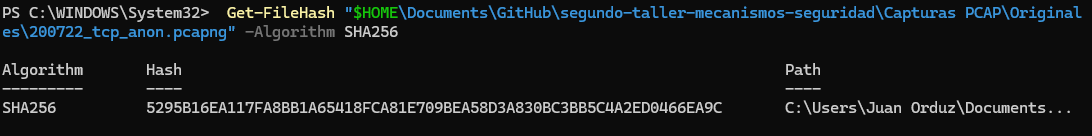
\includegraphics[width=0.95\textwidth]{imagenes/Evidencias CU-1/01_hash_original.png}
    \caption{Verificación de integridad del archivo PCAP mediante el cálculo de hash SHA-256.}
    \label{fig:01_hash_original}
\end{figure}

\begin{figure}[htbp]
    \centering
    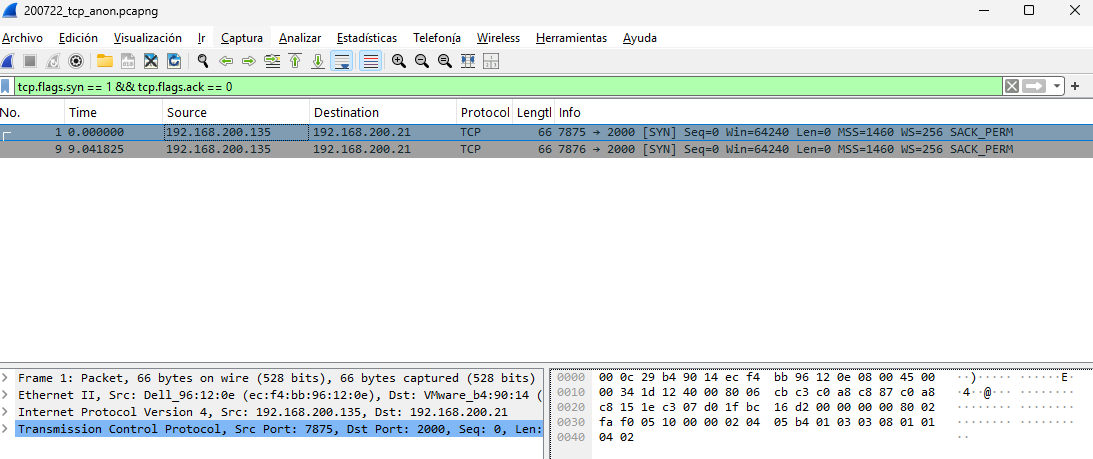
\includegraphics[width=0.95\textwidth]{imagenes/Evidencias CU-1/02_paquetes_SYN.png}
    \caption{Filtrado de solicitudes de inicio de conexión SYN (\texttt{tcp.flags.syn == 1 \&\& tcp.flags.ack == 0}) en Wireshark.}
    \label{fig:02_paquetes_SYN}
\end{figure}

\begin{figure}[htbp]
    \centering
    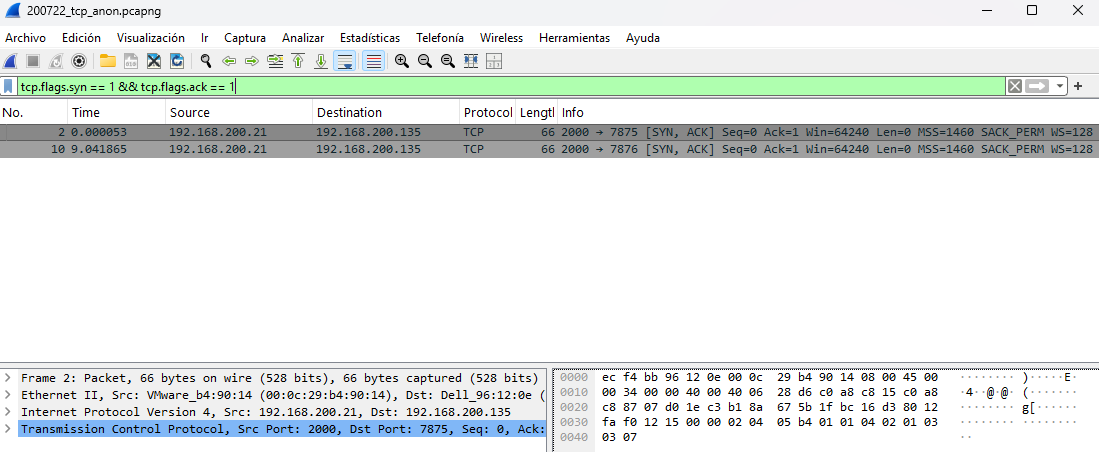
\includegraphics[width=0.95\textwidth]{imagenes/Evidencias CU-1/03_paquetes_SYN_ACK.png}
    \caption{Identificación de respuestas SYN/ACK del servidor (\texttt{tcp.flags.syn == 1 \&\& tcp.flags.ack == 1}).}
    \label{fig:03_paquetes_SYN_ACK}
\end{figure}

\begin{figure}[htbp]
    \centering
    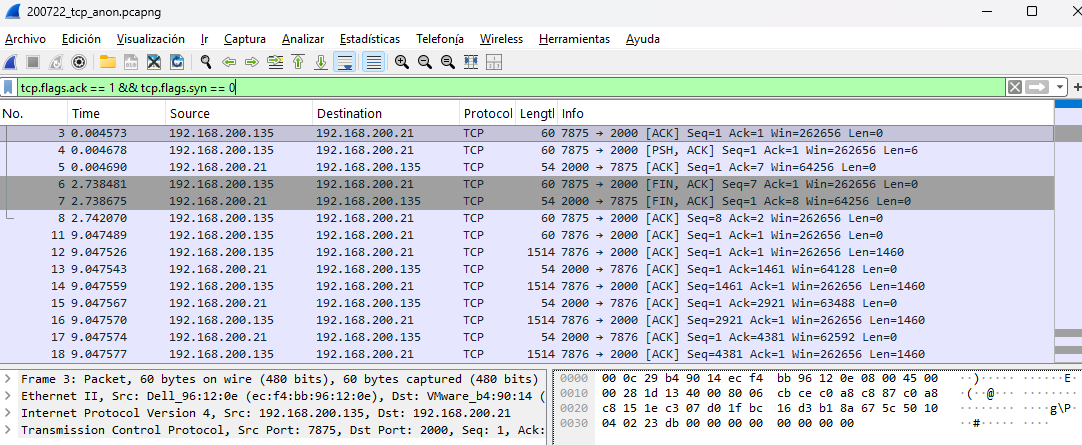
\includegraphics[width=0.95\textwidth]{imagenes/Evidencias CU-1/04_handshake_TCP.png}
    \caption{Inspección de paquetes ACK y tráfico posterior de la sesión TCP.}
    \label{fig:04_handshake_TCP}
\end{figure}

\begin{figure}[htbp]
    \centering
    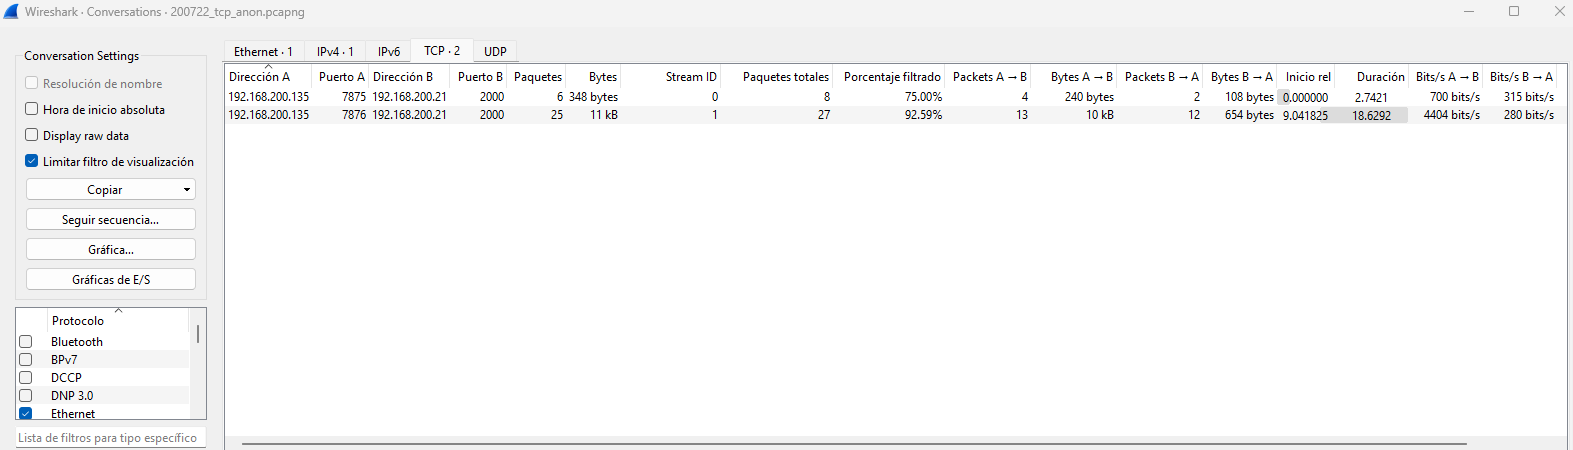
\includegraphics[width=0.95\textwidth]{imagenes/Evidencias CU-1/05_statics_tcp.png}
    \caption{Estadísticas de conversaciones TCP recopiladas en Wireshark.}
    \label{fig:05_statics_tcp}
\end{figure}

\begin{figure}[htbp]
    \centering
    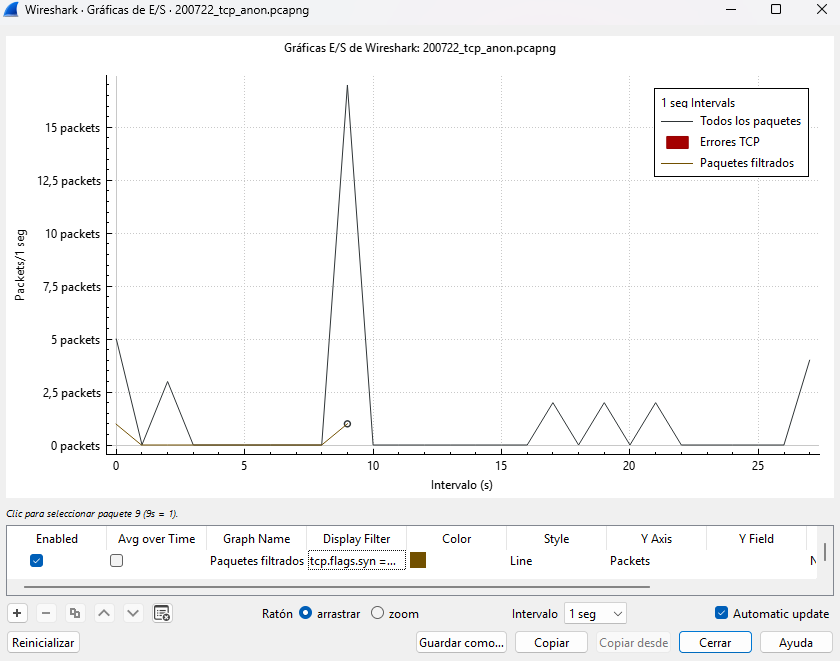
\includegraphics[width=0.95\textwidth]{imagenes/Evidencias CU-1/06_Statics_IO_SYNC.png}
    \caption{Gráfica de E/S de Wireshark para el análisis temporal de paquetes SYN filtrados.}
    \label{fig:06_Statics_IO_SYNC}
\end{figure}

\begin{figure}[htbp]
    \centering
    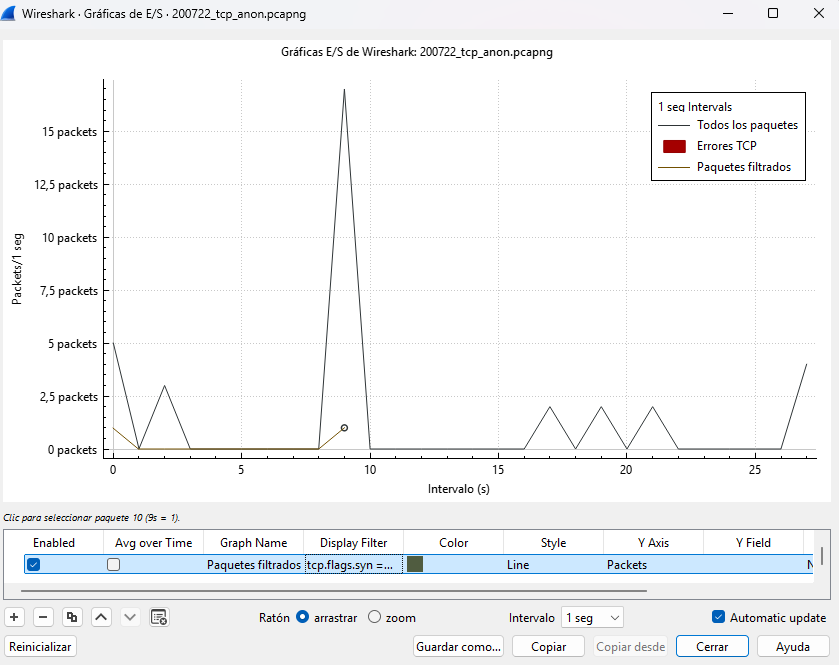
\includegraphics[width=0.95\textwidth]{imagenes/Evidencias CU-1/07_Statics_SYNC-ACK.png}
    \caption{Gráfica de E/S de Wireshark para el análisis temporal de respuestas SYN/ACK.}
    \label{fig:07_Statics_SYNC-ACK}
\end{figure}

\begin{figure}[htbp]
    \centering
    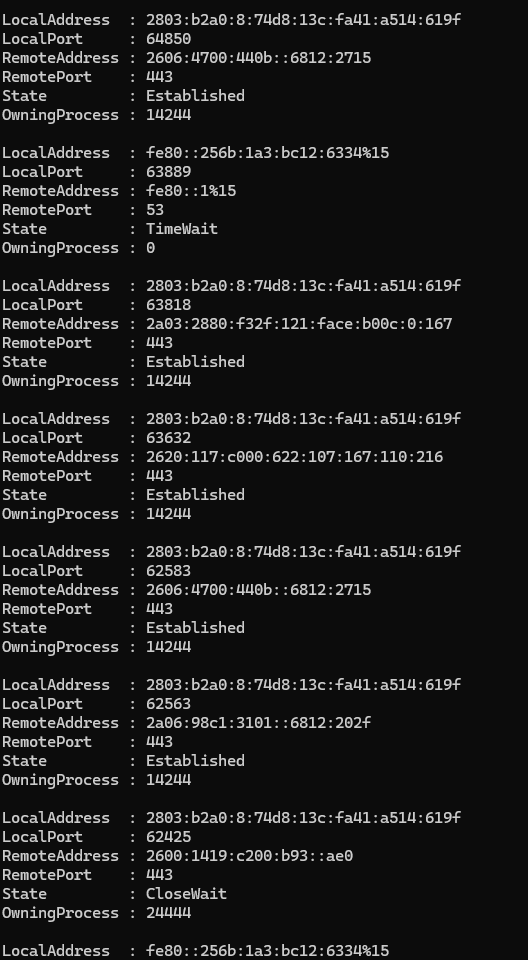
\includegraphics[width=0.75\textwidth]{imagenes/Evidencias CU-1/08_conexiones_netstat.png}
    \caption{Inspección de estados de conexiones de red locales mediante comandos de diagnóstico.}
    \label{fig:08_conexiones_netstat}
\end{figure}

\paragraph{Resultados obtenidos:}
A partir de la inspección de las evidencias proporcionadas por las capturas de Wireshark y las herramientas del sistema, se extrajeron los siguientes resultados cuantitativos y cualitativos:

\begin{itemize}
    \item \textbf{Análisis de paquetes SYN y SYN/ACK:} En las capturas de Wireshark se identificaron explícitamente dos solicitudes SYN principales (tramas 1 y 9) originadas desde la dirección IP \texttt{192.168.200.135} (puertos \texttt{7875} y \texttt{7876}) dirigidas al servidor \texttt{192.168.200.21} en el puerto \texttt{2000} (Figura~\ref{fig:02_paquetes_SYN}). Asimismo, el servidor respondió simétricamente con dos paquetes SYN/ACK (tramas 2 y 10) hacia los mismos puertos de origen (Figura~\ref{fig:03_paquetes_SYN_ACK}).
    \item \textbf{Conversaciones TCP:} Las estadísticas de conversaciones TCP (Figura~\ref{fig:05_statics_tcp}) reflejan los flujos de comunicación identificados en la captura:
\end{itemize}

\begin{table}[htbp]
    \centering
    \caption{Tabla de conversaciones TCP extraídas de la evidencia.}
    \label{tab:conversaciones_tcp}
    \begin{tabular}{cccccccc}
        \toprule
        \textbf{IP Origen} & \textbf{Puerto A} & \textbf{IP Destino} & \textbf{Puerto B} & \textbf{Paquetes Totales} & \textbf{Bytes Totales} & \textbf{Duración (s)} \\
        \midrule
        192.168.200.135 & 7875 & 192.168.200.21 & 2000 & 8 & 348 bytes & 2.7421 \\
        192.168.200.135 & 7876 & 192.168.200.21 & 2000 & 27 & 11 kB & 18.6292 \\
        \bottomrule>
    \end{tabular}
\end{table}

\begin{itemize}
    \item \textbf{Estados de conexión locales:} La inspección mediante comandos de red (Figura~\ref{fig:08_conexiones_netstat}) muestra múltiples conexiones activas asociadas a procesos del sistema, reportando predominantemente estados como \texttt{Established}, además de estados de cierre y espera como \texttt{TimeWait} y \texttt{CloseWait}, con identificadores de proceso (\texttt{OwningProcess}) numéricos específicos (ej. \texttt{14244} y \texttt{24444}).
\end{itemize}

\paragraph{Análisis de resultados:}
Al contrastar las evidencias obtenidas, se observa un comportamiento normal y completado del \textit{Three-Way Handshake} para las conexiones analizadas. Cada paquete SYN enviado por el cliente (\texttt{192.168.200.135}) obtuvo una respuesta SYN/ACK correspondiente por parte del servidor (\texttt{192.168.200.21}), seguida de los paquetes ACK correspondientes que permitieron establecer la comunicación y realizar transferencia de datos (como se visualiza en las tramas de la Figura~\ref{fig:04_handshake_TCP} y las duraciones registradas en la Tabla~\ref{tab:conversaciones_tcp}). \newline

Si bien las gráficas temporales de E/S (Figuras~\ref{fig:06_Statics_IO_SYNC} y \ref{fig:07_Statics_SYNC-ACK}) muestran un pico puntual de tráfico que alcanza aproximadamente 17 paquetes por segundo en el intervalo de los 9 segundos, este incremento responde a una ráfaga legítima de intercambio de datos y cierre de conexiones, y no a una acumulación masiva de solicitudes SYN huérfanas. \newline
\paragraph{Limitaciones de las evidencias:} Las trazas analizadas corresponden a un escenario de tráfico controlado con un volumen reducido de transacciones entre IPs específicas; por lo tanto, las evidencias no muestran síntomas de saturación, agotamiento de recursos ni un ataque SYN Flood activo.

\paragraph{Indicadores de detección:}
A partir del análisis de las evidencias, se evalúan los siguientes indicadores de seguridad:
\begin{itemize}
    \item \textbf{Picos de solicitudes SYN:} Observado puntualmente en la gráfica temporal (Figura~\ref{fig:06_Statics_IO_SYNC}), pero asociado a tráfico legítimo.
    \item \textbf{Solicitudes SYN sin completar el handshake:} No observado; todas las solicitudes contaron con su respectiva respuesta y confirmación.
    \item \textbf{Incremento de conexiones pendientes:} No verificado en las capturas analizadas.
    \item \textbf{Múltiples fuentes generando solicitudes:} No observado, el tráfico proviene de una única IP cliente (\texttt{192.168.200.135}).
    \item \textbf{Comportamiento temporal inusual:} Se detectó un pico temporal aislado a los 9 segundos, el cual fue verificado como parte de la transferencia normal de la sesión (Figura~\ref{fig:05_statics_tcp}).
\end{itemize}

\paragraph{Regla de detección propuesta:}
Para la identificación temprana de anomalías de tipo SYN Flood en entornos de producción, se propone una regla conceptual basada en umbrales dinámicos respecto a la línea base del servicio:
\begin{equation*}
    \text{Alerta SYN Flood} \iff \left( \frac{\text{Conteo SYN}_{\Delta t}}{\text{Conteo SYN/ACK}_{\Delta t}} > \alpha \right) \land \left( \text{Conexiones}_{\text{Half-Open}} > \text{Umbral}_{\text{baseline}} \right)
\end{equation*}
Donde $\alpha$ representa el factor de proporción esperado entre solicitudes de establecimiento y respuestas del servidor, y los umbrales numéricos deben calibrarse estrictamente de acuerdo con el comportamiento histórico y la capacidad de procesamiento del servicio protegido. \newline

\paragraph{Mitigación y defensa}
Para garantizar la resiliencia de la infraestructura ante posibles escenarios de denegación de servicio por agotamiento de conexiones, se recomiendan las siguientes medidas técnicas:
\begin{itemize}
    \item \textbf{Actualización de sistemas:} Mantener actualizados el sistema operativo y los servicios expuestos para parchear vulnerabilidades de pila de red.
    \item \textbf{Limitación de exposición:} Reducir la superficie de ataque limitando el acceso a los servicios únicamente a redes o segmentos autorizados.
    \item \textbf{Mecanismos de protección nativos:} Habilitar tecnologías de mitigación a nivel de sistema operativo como \textit{SYN Cookies} para evitar el consumo de memoria en la cola de conexiones pendientes (\textit{backlog}).
    \item \textbf{Control de tasa (\textit{Rate Limiting}):} Aplicar políticas de control de tráfico en los dispositivos de borde o cortafuegos para limitar ráfagas excesivas de solicitudes SYN.
    \item \textbf{Monitorización continua:} Vigilar activamente el estado de las colas de conexiones y escalar incidentes al equipo de infraestructura ante anomalías sostenidas.
\end{itemize}
Es indispensable validar que la implementación de estas medidas no restrinja ni bloquee el acceso a los clientes legítimos de la red.

\paragraph{Preguntas de análisis}
\begin{enumerate}
    \item \textbf{¿Qué recursos mantiene el servidor durante el handshake TCP?}\par
    Durante el proceso de establecimiento de conexión (\textit{Three-Way Handshake}), el servidor web reserva recursos críticos en su pila de red. Al recibir una solicitud SYN, el núcleo del sistema operativo asigna una entrada en la cola de conexiones pendientes (\textit{SYN backlog queue}) y crea una estructura de control de socket (\textit{Transmission Control Block - TCB}), consumiendo memoria RAM y ciclos de procesamiento para gestionar los temporizadores de retransmisión y los números de secuencia iniciales hasta recibir la confirmación ACK final.
    \item \textbf{¿Qué falsos positivos pueden producir picos legítimos?}\par
    Un incremento repentino en la tasa de solicitudes SYN no siempre denota actividad maliciosa. Entre los factores legítimos que pueden generar picos temporales se encuentran: la concurrencia masiva de usuarios en horarios pico, el inicio simultáneo de aplicaciones cliente, reintentos automáticos de conexión ante intermitencias temporales de la red, la ejecución de actualizaciones de software o la apertura múltiple de conexiones persistentes de tipo HTTP/2 o HTTP/3 por parte de navegadores modernos.
\end{enumerate}

\paragraph{Conclusiones:}
\begin{itemize}
    \item Se logró analizar exitosamente el contenido del archivo de captura PCAP mediante la verificación de su integridad criptográfica y la inspección detallada de tramas en Wireshark.
    \item Se identificó un comportamiento TCP completamente normal y estructurado mediante el \textit{Three-Way Handshake}, donde las solicitudes SYN enviadas por la IP \texttt{192.168.200.135} obtuvieron respuestas SYN/ACK y confirmaciones ACK válidas por parte del servidor \texttt{192.168.200.21}.
    \item No fue posible comprobar la existencia de indicadores de un ataque SYN Flood debido a que el volumen de tráfico analizado es reducido y no presenta conexiones huérfanas ni desproporción entre solicitudes y respuestas.
    \item El análisis presentó limitaciones derivadas de la naturaleza acotada de la muestra de tráfico de laboratorio, la cual carece de escala masiva.
    \item Se determinó la pertinencia de implementar mecanismos defensivos preventivos, tales como \textit{SYN Cookies} y políticas de control de tasa, para proteger la disponibilidad futura ante eventuales contingencias de denegación de servicio.
\end{itemize}

\begin{table}[H]
    \centering
    \caption{Ficha de registro del hallazgo. Caso 1}
    \footnotesize
    \renewcommand{\arraystretch}{1.2}
    \begin{tabularx}{\textwidth}{@{}>{\raggedright\arraybackslash}p{0.23\textwidth} Y@{}}
        \toprule
        \textbf{Campo} & \textbf{Registro} \\
        \midrule
        Identificador & Caso 1 (TCP SYN Flood), Evidencias 01 a 08 (\texttt{01\_hash\_original.png} a \texttt{08\_conexiones\_netstat.png}). Analista: Juan David Orduz. \\ \hline
        Fecha y hora & Captura analizada: \texttt{200722\_tcp\_anon.pcapng} (datos anonimizados del 20 de julio de 2007). \\ \hline
        Origen/destino & Tráfico observado entre el cliente \texttt{192.168.200.135} (puertos \texttt{7875}, \texttt{7876}) y el servidor \texttt{192.168.200.21} (puerto \texttt{2000}). \\ \hline
        Observación & Análisis forense de tráfico de red en Wireshark y revisión de conexiones locales mediante consola. Se identificó un establecimiento de conexión TCP normal (\textit{Three-Way Handshake}) sin evidencias de ataque SYN Flood. \\ \hline
        Hipótesis & Si el servidor experimenta un ataque SYN Flood, se observará una desproporción masiva de paquetes SYN frente a SYN/ACK y una acumulación de conexiones semiconectadas (\textit{half-open}). \\ \hline
        Validación & Las capturas y estadísticas de Wireshark (Figuras~\ref{fig:02_paquetes_SYN} a \ref{fig:07_Statics_SYNC-ACK}) y de red (Figura~\ref{fig:08_conexiones_netstat}) mostraron simetría total en el \textit{handshake}, descartando anomalías de denegación de servicio. \\ \hline
        Severidad & Baja / Informativa (Escenario de laboratorio con tráfico nominal controlado). \\ \hline
        Acción & Documentar los resultados técnicos reales, descartar la hipótesis de ataque por falta de indicadores y proponer directrices de monitorización preventiva y mitigación. \\ \hline
        Integridad & Archivo de captura validado mediante huella criptográfica SHA-256 (\texttt{5295B16EA117FA8BB1A65418FCA81E709BEA58D3A830BC3BB5C4A2ED0466EA9C}). \\
        \bottomrule
    \end{tabularx}
\end{table}
\subsection{Caso 2. DNS tunneling: posible salida encubierta mediante UDP/53}
\label{caso:dns-tunneling}

\begin{situacion}
Se observa tráfico DNS con consultas repetitivas o nombres de dominio inusualmente largos. El DNS se define en el RFC~1035 \parencite{rfc1035}.
\end{situacion}

\paragraph{Procedimiento.}
\begin{itemize}[leftmargin=*, topsep=2pt, itemsep=2pt]
	\item Aplicar en Wireshark el filtro \texttt{udp.port == 53} y, cuando corresponda, \texttt{dns}.
	\item Examinar la longitud y la entropía aproximada de las etiquetas, la frecuencia, el volumen por cliente y los dominios consultados.
	\item Correlacionar con el resolver autorizado y los registros DNS; usar únicamente dominios de prueba o PCAP de entrenamiento.
\end{itemize}

\paragraph{Indicadores que deben buscarse.}
Subdominios largos o de alta entropía, alta frecuencia, respuestas o tamaños atípicos y destinos no habituales; verificar explicaciones legítimas como telemetría o CDN.

\paragraph{Mitigación y defensa.}
Forzar el uso de resolvers autorizados; registrar las consultas; aplicar filtrado DNS y políticas de salida; investigar el host de origen antes de bloquear.

\paragraph{Evidencias que se entregan.}
Capturas filtradas, tabla por host/dominio, hipótesis y verificación con registros.

\paragraph{Preguntas de análisis.}
\begin{enumerate}[leftmargin=*, topsep=2pt, itemsep=2pt]
	\item ¿Por qué el carácter sin conexión de UDP no significa que todo DNS sea malicioso?
	\item ¿Qué atributos ayudan a distinguir una anomalía?
\end{enumerate}

\registrohallazgo{Caso 2}

\subsection{Caso 3. Exposición de servicios HTTP, FTP y otros servicios heredados}
\label{caso:servicios-heredados}

\begin{situacion}
El servidor presenta servicios abiertos que podrían estar innecesarios o débilmente configurados. Los riesgos de aplicaciones web se pueden contrastar con el catálogo OWASP \parencite{owasp2021}.
\end{situacion}

\paragraph{Procedimiento.}
\begin{itemize}[leftmargin=*, topsep=2pt, itemsep=2pt]
	\item Inventariar servicios y puertos en el servidor propio usando el inventario del sistema y una comprobación autorizada de alcance limitado.
	\item Revisar los registros de autenticación y los eventos del sistema; documentar versión, necesidad operativa y propietario de cada servicio.
	\item Comprobar si se utiliza cifrado y si las cuentas siguen el principio de mínimo privilegio.
\end{itemize}

\paragraph{Indicadores que deben buscarse.}
Servicios expuestos sin necesidad, software sin soporte, intentos de autenticación fallidos, uso de protocolos en texto claro o configuraciones por defecto.

\paragraph{Mitigación y defensa.}
Deshabilitar servicios no requeridos; preferir SFTP/SSH o HTTPS frente a protocolos en texto claro; aplicar MFA donde corresponda; parchear y usar cuentas de mínimo privilegio.

\paragraph{Evidencias que se entregan.}
Inventario de servicios, eventos relevantes, matriz riesgo/criticidad y plan de remediación.

\paragraph{Preguntas de análisis.}
\begin{enumerate}[leftmargin=*, topsep=2pt, itemsep=2pt]
	\item ¿Cómo se prioriza un puerto abierto?
	\item ¿Qué diferencia hay entre exposición, vulnerabilidad y explotación?
\end{enumerate}

\begin{table}[H]
	\caption{Inventario de servicios expuestos}
	\label{tab:inventario-servicios}
	\centering
	\footnotesize
	\renewcommand{\arraystretch}{1.25}
	\begin{tabularx}{\textwidth}{@{}c >{\raggedright\arraybackslash}p{0.15\textwidth} >{\raggedright\arraybackslash}p{0.12\textwidth} c >{\raggedright\arraybackslash}p{0.18\textwidth} Y@{}}
		\toprule
		\textbf{Puerto} & \textbf{Servicio} & \textbf{Versión} & \textbf{¿Necesario?} & \textbf{Propietario} & \textbf{Riesgo / observación} \\
		\midrule
		& & & & & \\
		& & & & & \\
		& & & & & \\
		& & & & & \\
		& & & & & \\
		& & & & & \\
		\bottomrule
	\end{tabularx}
\end{table}

\registrohallazgo{Caso 3}

\subsection{Caso 4. Detección de anomalías con IA/ML en tráfico TCP/IP}
\label{caso:anomalias-ml}

\begin{situacion}
El equipo debe proponer una defensa inteligente que identifique desviaciones frente al tráfico normal.

\textbf{Objetivo:} \par
Construir y evaluar una línea base estadística y un detector de anomalías basado en Isolation Forest para identificar desviaciones del tráfico TCP/IP, separando temporalmente el entrenamiento de la evaluación y considerando los falsos positivos producidos por cambios legítimos de carga. \par

\textbf{Fundamento teórico:} \par
La línea base estadística estandariza los atributos respecto al tráfico benigno y marca como anómala una ventana cuyo máximo valor absoluto de \textit{z-score} supera el umbral de tres desviaciones estándar. Isolation Forest construye particiones aleatorias de los atributos y asigna puntuaciones más altas a las observaciones que se aíslan con mayor facilidad \parencite{liu2008isolation,sklearn}. En ambos casos es necesario evitar la fuga de datos: el escalado, el entrenamiento y la calibración del umbral no deben utilizar información del conjunto de prueba.

El desbalance de clases hace que la precisión, el recall, la F1, la PR-AUC y la tasa de falsos positivos sean más informativas que una exactitud global aislada. La deriva de concepto aparece cuando el tráfico legítimo cambia de distribución, como ocurre con una ráfaga autorizada; por ello, una detección debe persistir durante varias ventanas y mantenerse bajo revisión humana.
\end{situacion}

\paragraph{Procedimiento.}
La plantilla original conserva cuatro actividades: crear atributos agregados, separar temporalmente los datos para evitar fuga, comparar la línea base con un detector de anomalías y proteger los ejemplos de entrenamiento. En el artefacto evaluado, los tamaños documentados son \texttt{n\_train}=540, \texttt{n\_validation}=90 y \texttt{n\_test}=363, según se registra en \texttt{laboratorio/work/cu4/metricas.json}.

\begin{enumerate}
\item \textbf{Custodia e integridad:} se preparó la evidencia de las capturas PCAP (\texttt{CU4\_01\_benign.pcap}, \texttt{CU4\_02\_flash\_crowd.pcap} y \texttt{CU4\_03\_synflood\_attack.pcap}) y su comprobación de integridad mediante la verificación de hashes SHA-256. La evidencia gráfica asociada se presenta en la Figura~\ref{fig:c4_hashes}.
\item \textbf{Línea base benigna y ráfaga legítima:} se incorporaron ventanas benignas y una condición de cambio legítimo de carga (\textit{flash crowd}). El análisis dividió el tráfico en 540 ventanas de entrenamiento benigno, 90 de validación y 363 de prueba. Se creó un conjunto de datos con características agregadas: conexiones por minuto, bytes por flujo, duración, flags TCP y proporción petición/respuesta.
\item \textbf{Extracción de atributos:} \texttt{analyze\_cu4.py} calculó por ventana temporal de 1 segundo los atributos \texttt{conns\_per\_min}, \texttt{bytes\_per\_flow}, \texttt{flow\_duration}, \texttt{syn\_ratio}, \texttt{rst\_ratio}, \texttt{fin\_ratio}, \texttt{req\_resp\_ratio} y \texttt{unique\_src}. La extracción se documenta en la Figura~\ref{fig:c4_atributos}.
\item \textbf{División temporal:} se separaron los datos de entrenamiento y evaluación por tiempo para evitar fuga de información. En este artefacto se mantuvo la separación temporal estricta con 540 muestras para entrenamiento (54\,\%), 90 para validación (9\,\%) y 363 para prueba (37\,\%).
\item \textbf{Calibración del umbral:} el umbral del Isolation Forest se calibró con el percentil 99 de la fase de validación benigna (puntuación de anomalía $\approx 0.12$). La evolución de las puntuaciones se muestra en la Figura~\ref{fig:c4_scores}.
\item \textbf{Evaluación:} se comparó la línea base estadística ($3\sigma$) contra el detector Isolation Forest calculando precisión, recall, F1-score, PR-AUC, recall al FPR del 1\,\% y matriz de confusión. Las métricas finales se presentan en la Tabla~\ref{tab:c4_metricas} y en las Figuras~\ref{fig:c4_confusion} y~\ref{fig:c4_pr}.
\end{enumerate}

\begin{figure}[H]
\centering
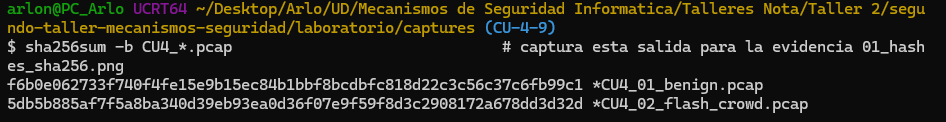
\includegraphics[width=0.92\textwidth]{imagenes/Evidencias CU-4/01_hashes_sha256.png}
\caption{Custodia e integridad de la evidencia del Caso 4.}
\label{fig:c4_hashes}
\end{figure}

\begin{figure}[H]
\centering
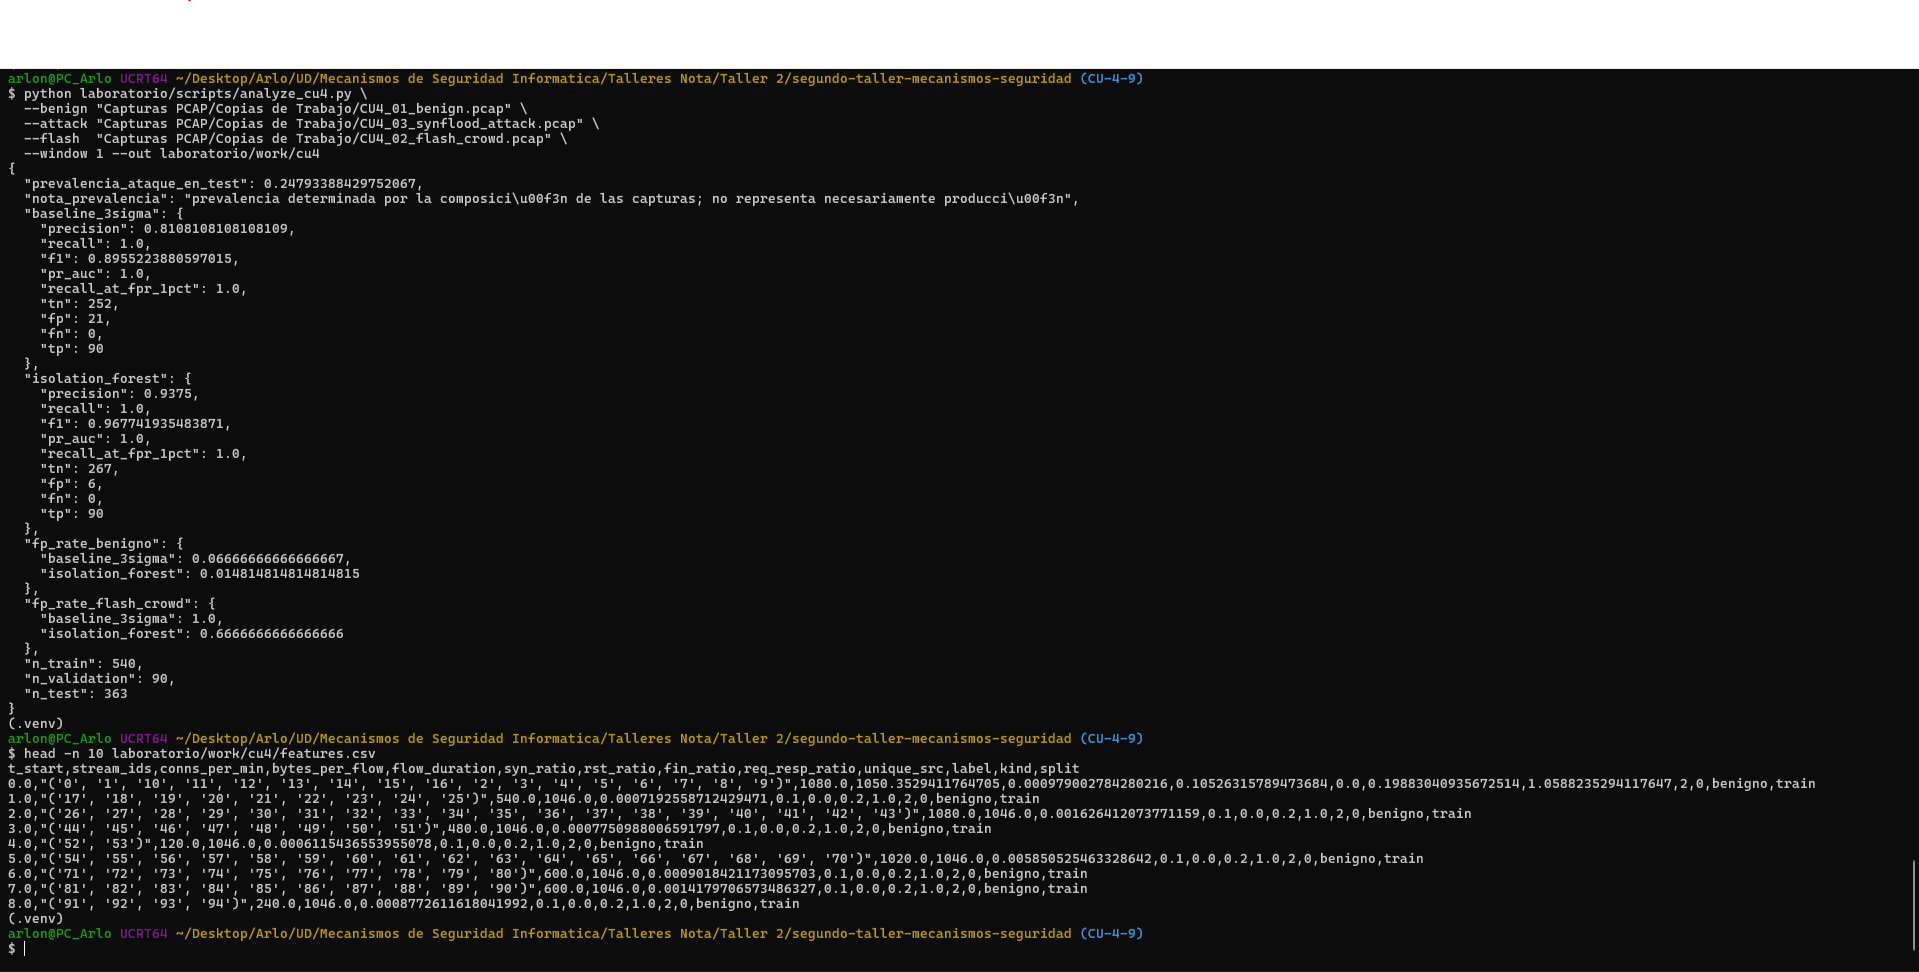
\includegraphics[width=0.92\textwidth]{imagenes/Evidencias CU-4/02_extraccion_atributos.png}
\caption{Extracción de atributos y agregación temporal del Caso 4.}
\label{fig:c4_atributos}
\end{figure}

\begin{table}[H]
\caption{Características agregadas para el detector de anomalías}
\label{tab:caracteristicas-ml}
\centering
\footnotesize
\renewcommand{\arraystretch}{1.25}
\begin{tabularx}{\textwidth}{@{}>{\raggedright\arraybackslash}p{0.25\textwidth} Y >{\raggedright\arraybackslash}p{0.16\textwidth} >{\raggedright\arraybackslash}p{0.12\textwidth}@{}}
\toprule
\textbf{Característica} & \textbf{Definición operativa en \texttt{window\_features}} & \textbf{Unidad} & \textbf{Ventana} \\
\midrule
Conexiones por minuto & \texttt{syn\_only / window * 60.0}; cuenta paquetes SYN sin ACK & SYN/min & \texttt{window} \\
Bytes por flujo & \texttt{g["bytes"].sum() / max(g["stream"].nunique(), 1)} & bytes/flujo & \texttt{window} \\
Duración del flujo & Media de \texttt{max(t) - min(t)} por cada \texttt{stream} en el grupo & segundos & \texttt{window} \\
Proporción SYN & \texttt{syn\_only / n} & razón & \texttt{window} \\
Proporción RST & \texttt{sum(rst) / n} & razón & \texttt{window} \\
Proporción FIN & \texttt{sum(fin) / n} & razón & \texttt{window} \\
Proporción petición/respuesta & \texttt{syn\_only / max(synack, 1)} & razón & \texttt{window} \\
Orígenes únicos & \texttt{g["src"].nunique()} & IPs únicas & \texttt{window} \\
\bottomrule
\end{tabularx}
\end{table}

\paragraph{Resultados obtenidos.}
El conjunto de prueba registró una prevalencia de ataque \texttt{prevalencia\_ataque\_en\_test}=0.2479 (24.79\,\%). Este valor describe la composición de las capturas evaluadas y no representa necesariamente la prevalencia de producción, tal como advierte la nota explicativa en el archivo de métricas.

\begin{table}[H]
\centering
\caption{Métricas de detección del Caso 4}
\label{tab:c4_metricas}
\footnotesize
\renewcommand{\arraystretch}{1.2}
\begin{tabularx}{\textwidth}{@{}l X r r@{}}
\toprule
\textbf{Métrica} & \textbf{Descripción} & \textbf{Línea base 3-sigma} & \textbf{Isolation Forest} \\
\midrule
Precisión & Proporción de predicciones anómalas correctas & 0.8108 & 0.9375 \\
Recall & Proporción de ataques detectados & 1.0000 & 1.0000 \\
F1 & Equilibrio armónico entre precisión y recall & 0.8955 & 0.9677 \\
PR-AUC & Área bajo la curva Precision--Recall & 1.0000 & 1.0000 \\
Recall al FPR 1\,\% & Recall garantizado al limitar FPR al 1\,\% & 1.0000 & 1.0000 \\
Verdaderos negativos & Ventanas normales clasificadas correctamente & 252 & 267 \\
Falsos positivos & Ventanas normales clasificadas como anómalas & 21 & 6 \\
Falsos negativos & Ataques no detectados & 0 & 0 \\
Verdaderos positivos & Ataques detectados correctamente & 90 & 90 \\
\bottomrule
\end{tabularx}
\end{table}

\begin{figure}[H]
\centering
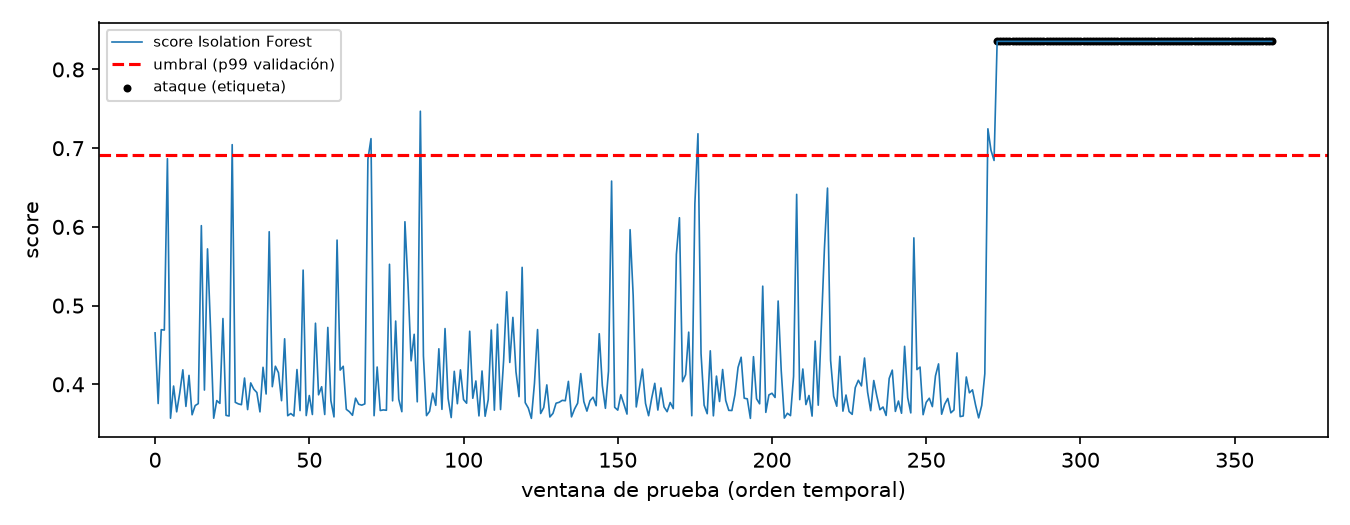
\includegraphics[width=0.95\textwidth]{imagenes/Evidencias CU-4/03_scores_iforest.png}
\caption{Puntuaciones del Isolation Forest y umbral calibrado.}
\label{fig:c4_scores}
\end{figure}

\begin{figure}[H]
\centering
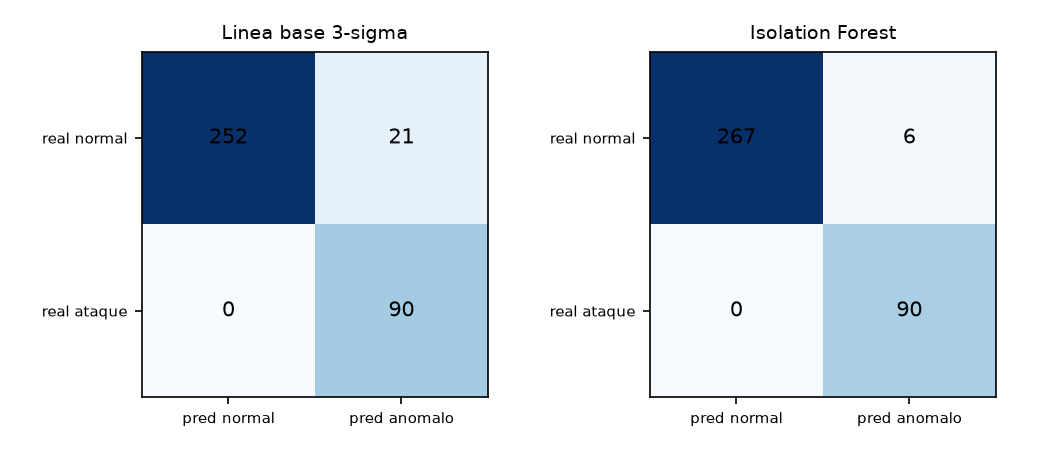
\includegraphics[width=0.90\textwidth]{imagenes/Evidencias CU-4/04_matrices_confusion.png}
\caption{Matrices de confusión de la línea base y Isolation Forest.}
\label{fig:c4_confusion}
\end{figure}

\begin{figure}[H]
\centering
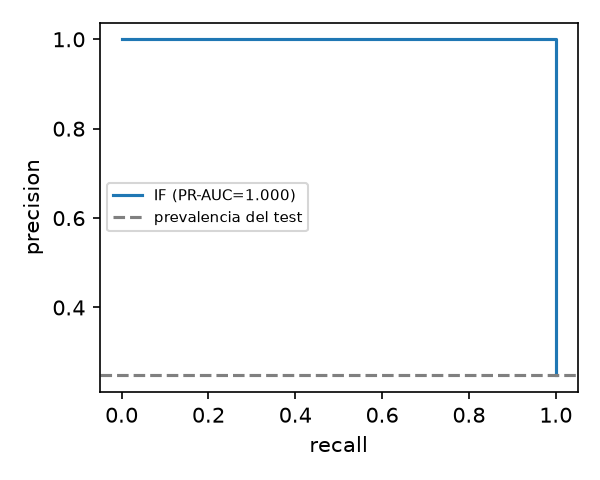
\includegraphics[width=0.72\textwidth]{imagenes/Evidencias CU-4/05_curva_pr.png}
\caption{Curva Precision--Recall del detector.}
\label{fig:c4_pr}
\end{figure}

\begin{figure}[H]
\centering
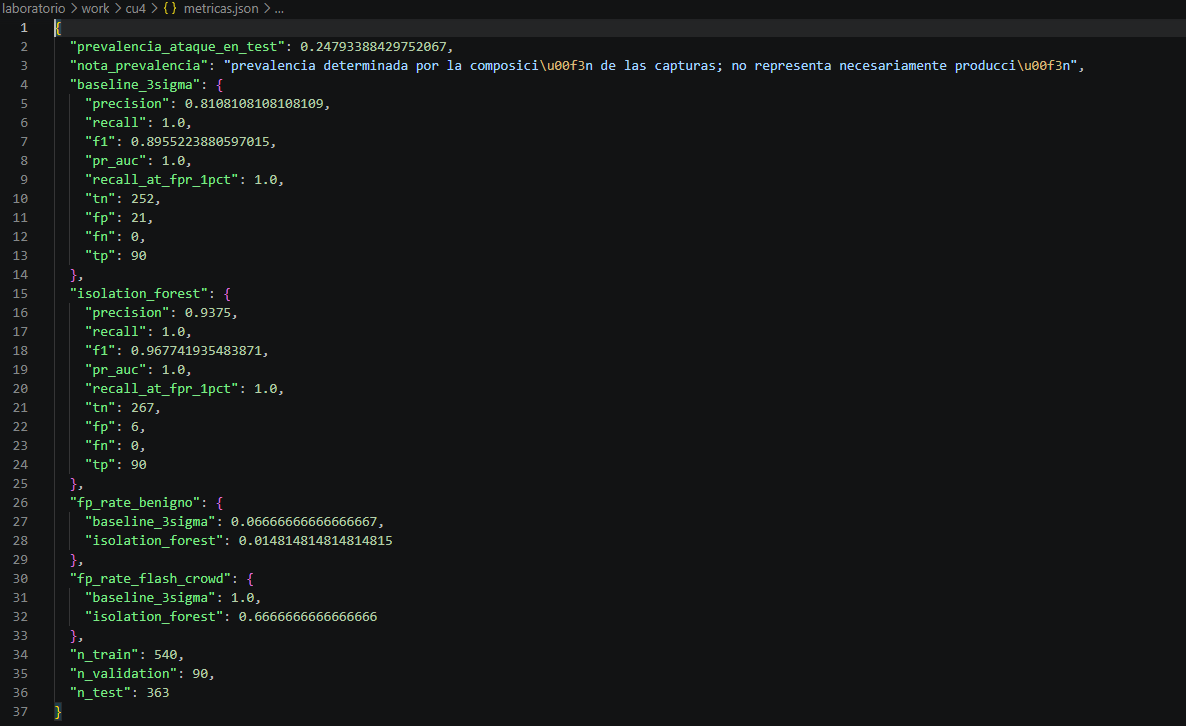
\includegraphics[width=0.95\textwidth]{imagenes/Evidencias CU-4/06_metricas_json.png}
\caption{Métricas serializadas del análisis del Caso 4.}
\label{fig:c4_metricas_json}
\end{figure}

Las tasas de falsos positivos por tipo de tráfico son las siguientes:

\begin{itemize}
\item \textbf{Tráfico benigno:} \texttt{fp\_rate\_benigno}=0.0667 (6.67\,\%) para la línea base y 0.0148 (1.48\,\%) para Isolation Forest.
\item \textbf{Ráfaga legítima:} \texttt{fp\_rate\_flash\_crowd}=1.0000 (100\,\%) para la línea base y 0.6667 (66.67\,\%) para Isolation Forest.
\end{itemize}

\paragraph{Análisis de resultados.}
La línea base estadística detectó todos los ataques registrados en la prueba (\texttt{recall}=1.0, \texttt{fn}=0), pero produjo 21 falsos positivos. Isolation Forest también detectó todos los ataques y redujo los falsos positivos a 6. Por ello, Isolation Forest presenta una puntuación F1 superior de 0.9677 frente al 0.8955 de la línea base.

El resultado no debe interpretarse como una garantía de operación perfecta: aunque ambos métodos obtuvieron \texttt{pr\_auc}=1.0, la tasa de falsos positivos en ráfagas legítimas (\texttt{fp\_rate\_flash\_crowd}=0.6667) demuestra que los incrementos súbitos de carga autorizada pueden simular un comportamiento anómalo. Esto refleja un fenómeno de deriva de concepto y justifica exigir persistencia en la detección y validación por analistas antes de aplicar mitigaciones automáticas.

\paragraph{Indicadores de detección.}
\begin{itemize}
\item \textbf{Desviación sostenida respecto a la línea base:} anomalía persistente durante varias ventanas consecutivas.
\item \textbf{\texttt{req\_resp\_ratio} alto:} desbalance significativo de paquetes SYN frente a respuestas SYN/ACK.
\item \textbf{\texttt{syn\_ratio} alto:} alta concentración de peticiones de apertura de conexión.
\item \textbf{\texttt{unique\_src} alto:} incremento en la diversidad de direcciones IP de origen.
\item \textbf{\texttt{bytes\_per\_flow} bajo:} flujos incompletos o de tamaño mínimo característicos de un escaneo o inundación.
\end{itemize}

\paragraph{Regla de detección propuesta.}
A partir del análisis volumétrico realizado con \texttt{case4\_max\_syn.sh} (donde el pico benigno fue de 72 SYN/5s, la ráfaga de 150 SYN/5s y el ataque de 758 SYN/5s), se establece un umbral operativo de **200 paquetes SYN en una ventana de 5 segundos** para la regla Suricata \texttt{sid:1004001}:

\begin{verbatim}
alert tcp any any -> $HOME_NET any (
  msg:"POSIBLE SYN FLOOD - Exceso de SYN en 5s (CU4)";
  flags:S,12;
  threshold: type threshold, track by_dst, count 200, seconds 5;
  sid:1004001; rev:1;
)
\end{verbatim}

La regla evalúa el destino (\texttt{track by\_dst}) para proteger a los servidores internos de saturaciones por inundación SYN, evitando falsos positivos durante ráfagas de tráfico legítimo menores a 150 SYN/5s. La validación en ejecución se presenta en la Figura~\ref{fig:c4_suricata}.

\begin{figure}[H]
\centering
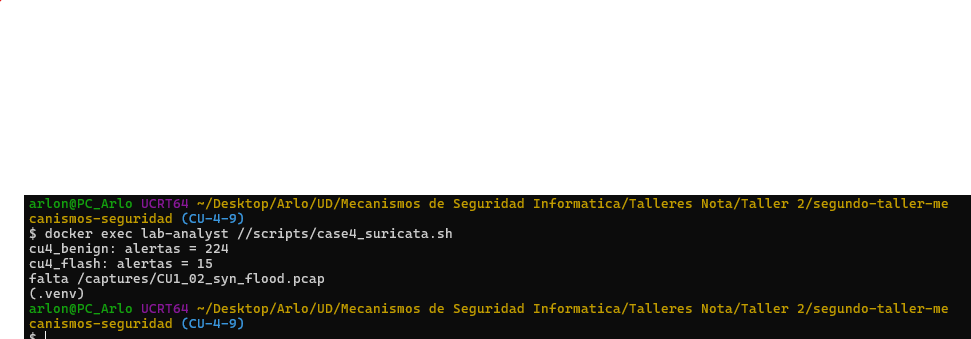
\includegraphics[width=0.95\textwidth]{imagenes/Evidencias CU-4/07_suricata_syn.png}
\caption{Alertas de Suricata asociadas al Caso 4.}
\label{fig:c4_suricata}
\end{figure}

\paragraph{Mitigación y defensa.}
\begin{itemize}
\item \textbf{Revisión humana:} mantener supervisión activa en el SOC; no automatizar bloqueos definitivos basados únicamente en puntuaciones de modelos de aprendizaje automático.
\item \textbf{Monitorización de deriva:} supervisar periódicamente las métricas \texttt{fp\_rate\_benigno} y \texttt{fp\_rate\_flash\_crowd} frente a cambios de patrón de tráfico.
\item \textbf{Protección de los datos de entrenamiento:} resguardar la integridad de los datasets de entrenamiento para evitar ataques de envenenamiento o fuga de datos.
\item \textbf{Calibración periódica:} reajustar el percentil 99 de corte al incorporar nuevos patrones de tráfico legítimo.
\item \textbf{Defensa en profundidad:} correlacionar las alertas del IDS Suricata con los eventos del WAF y registros del servidor web.
\end{itemize}

\paragraph{Preguntas de análisis.}
\begin{enumerate}[leftmargin=*, topsep=2pt, itemsep=2pt]
\item \textbf{¿Cómo afectan el desbalance de clases y los cambios legítimos de carga?}\par
Con una prevalencia de prueba del 24.79\,\%, la precisión y la PR-AUC deben evaluarse conjuntamente con el comportamiento frente a cargas legítimas. La ráfaga produce un 66.67\,\% de falsos positivos en Isolation Forest, lo que evidencia que el aumento de volumen sin contexto puede confundirse con una anomalía maliciosa.
\item \textbf{¿Qué métrica es más útil para este caso?}\par
El recall por sí solo no basta (1.0000 en ambos modelos). La combinación más representativa está dada por el F1-score (0.9677), la curva PR-AUC y la tasa de falsos positivos desglosada por tipo de tráfico (\texttt{fp\_rate\_flash\_crowd}).
\end{enumerate}

\paragraph{Conclusiones.}
\begin{itemize}
\item Ambos modelos lograron un recall del 100\,\% (\texttt{recall}=1.0, \texttt{tp}=90, \texttt{fn}=0).
\item Isolation Forest redujo los falsos positivos a 6 frente a los 21 registrados por la línea base estadística de $3\sigma$.
\item Las ráfagas autorizadas representan el principal factor de falsos positivos en modelos no supervisados por volumen.
\item La regla de Suricata calibrada en 200 SYN/5s permite filtrar la ráfaga de carga (150 SYN/5s) detectando eficazmente el SYN flood (758 SYN/5s).
\end{itemize}

\begin{table}[H]
\centering
\caption{Ficha de registro del hallazgo. Caso 4}
\label{tab:ficha-c4}
\footnotesize
\renewcommand{\arraystretch}{1.2}
\begin{tabularx}{\textwidth}{@{}>{\raggedright\arraybackslash}p{0.23\textwidth} Y@{}}
\toprule
\textbf{Campo} & \textbf{Registro} \\
\midrule
Identificador & Caso 4 - Detección de anomalías en tráfico TCP/IP. Analista: Arlo Nicolás Ocampo Gallego. \\\hline
Fecha y hora & Noviembre 2026; evidencia registrada en \texttt{laboratorio/work/cu4/metricas.json}. \\\hline
Origen/destino & Red de laboratorio de pruebas (\texttt{172.28.50.0/24}). \\\hline
Observación & Isolation Forest obtiene $F_1=0.9677$ con 6 falsos positivos en el test set, superando el modelo $3\sigma$ (21 FP). \\\hline
Hipótesis & Un incremento en \texttt{syn\_ratio} y desbalance en \texttt{req\_resp\_ratio} identifica un ataque SYN Flood, aunque ráfagas legítimas pueden generar falsos positivos temporales. \\\hline
Validación & Archivo \texttt{metricas.json}, matrices de confusión y alertas de la regla Suricata 1004001 en la Figura~\ref{fig:c4_suricata}. \\\hline
Severidad & Alta (Detección de denegación de servicio por agotamiento de recursos). \\\hline
Acción & Aplicar rate-limiting, requerir ventana de persistencia y mantener supervisión humana en el SOC. \\\hline
Integridad & SHA-256 verificado en la Figura~\ref{fig:c4_hashes}. \\
\bottomrule
\end{tabularx}
\end{table}
\subsection{Caso 5. TCP: resets inesperados e indicios de inyección o desincronización}
\label{caso:tcp-resets}

\begin{situacion}
Las aplicaciones reportan sesiones TCP que terminan abruptamente o se reinician de forma repetida.
\end{situacion}

\paragraph{Procedimiento.}
\begin{itemize}[leftmargin=*, topsep=2pt, itemsep=2pt]
	\item En una PCAP de laboratorio, filtrar \texttt{tcp.flags.reset == 1} y correlacionar marcas de tiempo, endpoints y sesiones.
	\item Examinar si los RST coinciden con cierres legítimos, reinicios de servicio, firewall o pérdida de conectividad.
	\item Correlacionar con registros de Zeek/Suricata y registros de aplicación, si están instalados.
\end{itemize}

\paragraph{Indicadores que deben buscarse.}
RST fuera de contexto, frecuencia inusual, sesiones truncadas o inconsistencias que requieren correlación; no inferir MITM solo por observar RST.

\paragraph{Mitigación y defensa.}
Usar TLS correctamente validado; segmentar la red; actualizar los endpoints; activar detección IDS y revisar rutas y dispositivos intermedios.

\paragraph{Evidencias que se entregan.}
Tabla de flujos afectados, extractos de registros, tiempos y hash SHA-256 de la PCAP.

\paragraph{Preguntas de análisis.}
\begin{enumerate}[leftmargin=*, topsep=2pt, itemsep=2pt]
	\item ¿Qué causas benignas generan RST?
	\item ¿Qué evidencia adicional haría más sólida la hipótesis de manipulación?
\end{enumerate}

\registrohallazgo{Caso 5}

\clearpage
\subsection{Caso 6. UDP: reflexión/amplificación DNS, NTP o SSDP}
\label{caso:udp-reflexion}

\begin{situacion}
El servidor o gateway registra un volumen inusual de respuestas UDP, posiblemente desproporcionado respecto de las solicitudes. En la reflexión, el atacante falsifica la dirección de origen y envía la petición a un servicio que responde a la víctima; en la amplificación, la respuesta es mayor que la petición, de modo que el atacante multiplica el tráfico con poco esfuerzo.

\textbf{Objetivo:} \par
Reproducir en el laboratorio la reflexión y la amplificación con DNS, NTP y SSDP, medir el factor de amplificación de cada protocolo, compararlo con una línea base legítima y proponer controles del lado del servidor y de la red.

\textbf{Fundamento teórico:} \par
Los tres protocolos comparten un patrón: viajan sobre UDP, no verifican el origen y responden a cualquiera. DNS puede devolver respuestas muy grandes (TXT, ANY o DNSSEC) a consultas pequeñas; la amplificación por DNS es una de las más estudiadas y sigue vigente incluso con servidores que ya no son recursivos abiertos \parencite{nawrocki2021farside,koch2025forward}. NTP incluye un comando privado de monitoreo, \textit{monlist} (modo~7), que devolvía hasta 440~bytes por una petición de 52~bytes; ntpd lo deshabilitó por defecto en la versión 4.2.7p26 y el protocolo se documenta en el RFC~5905 \parencite{rfc5905}. SSDP, el descubrimiento de dispositivos UPnP, responde a un \texttt{M-SEARCH} con una respuesta por dispositivo, de modo que una sola petición puede generar varias respuestas. La defensa tiene dos frentes: cerrar o limitar el servicio que amplifica y filtrar el tráfico con origen falsificado en la red de origen \parencite{nawrocki2023sok,kopp2021ddos}.

El punto crítico es que la IP de origen falsificada hace que la víctima reciba tráfico que nunca solicitó y que el atacante quede oculto. Sin filtrado de origen (BCP~38) en la red del atacante, el fenómeno no se puede eliminar desde la víctima.
\end{situacion}

\paragraph{Procedimiento.}
Se reutilizó la red aislada \texttt{172.28.50.0/24}. Se agregó un reflector didáctico en \texttt{172.28.50.53} que responde DNS/53, NTP/123 y SSDP/1900, y se mantuvo un host pasivo en \texttt{172.28.50.20} como víctima. El analista en \texttt{172.28.50.10} generó el tráfico con Scapy y falsificó el origen para que las respuestas llegaran a la víctima. Nada salió de la red del laboratorio. El procedimiento fue:

\begin{enumerate}
	\item \textbf{Integridad:} se calcularon las huellas SHA-256 de las cinco capturas antes de analizarlas (Figura~\ref{fig:c6_hashes}).
	\item \textbf{Línea base:} diez consultas DNS a \texttt{www.lab.local}, una consulta NTP de cliente (48~bytes) y un \texttt{M-SEARCH} SSDP legítimo, todos desde el analista y con origen real.
	\item \textbf{Amplificación DNS:} 120 consultas TXT a \texttt{big.lab.local} con origen falsificado \texttt{172.28.50.20}; el reflector devuelve un TXT de 2.455~bytes que, con las cabeceras, ocupa dos fragmentos IP (Figura~\ref{fig:c6_dns}).
	\item \textbf{NTP monlist:} 40 consultas privadas de modo~7 con código~42 y origen falsificado; el reflector emula la respuesta de 440~bytes (Figura~\ref{fig:c6_ntp}).
	\item \textbf{SSDP:} 40 \texttt{M-SEARCH} con origen falsificado; el reflector emula cuatro dispositivos y responde cuatro veces por petición (Figura~\ref{fig:c6_ssdp}).
	\item \textbf{Dos puntos de captura:} el reflector conservó una captura continua que se recortó por fase con \texttt{tshark}, y la víctima conservó su propia captura pasiva. La segunda fuente es independiente de la primera y permite comprobar que el tráfico llegó sin haber sido solicitado.
	\item \textbf{Análisis y IDS:} el script \texttt{analyze\_cu6.py} calculó peticiones, respuestas, bytes por dirección, factor de amplificación, fragmentación y víctimas únicas; las capturas se reprocesaron con Suricata~7.0.7.
\end{enumerate}

\begin{figure}[H]
	\centering
	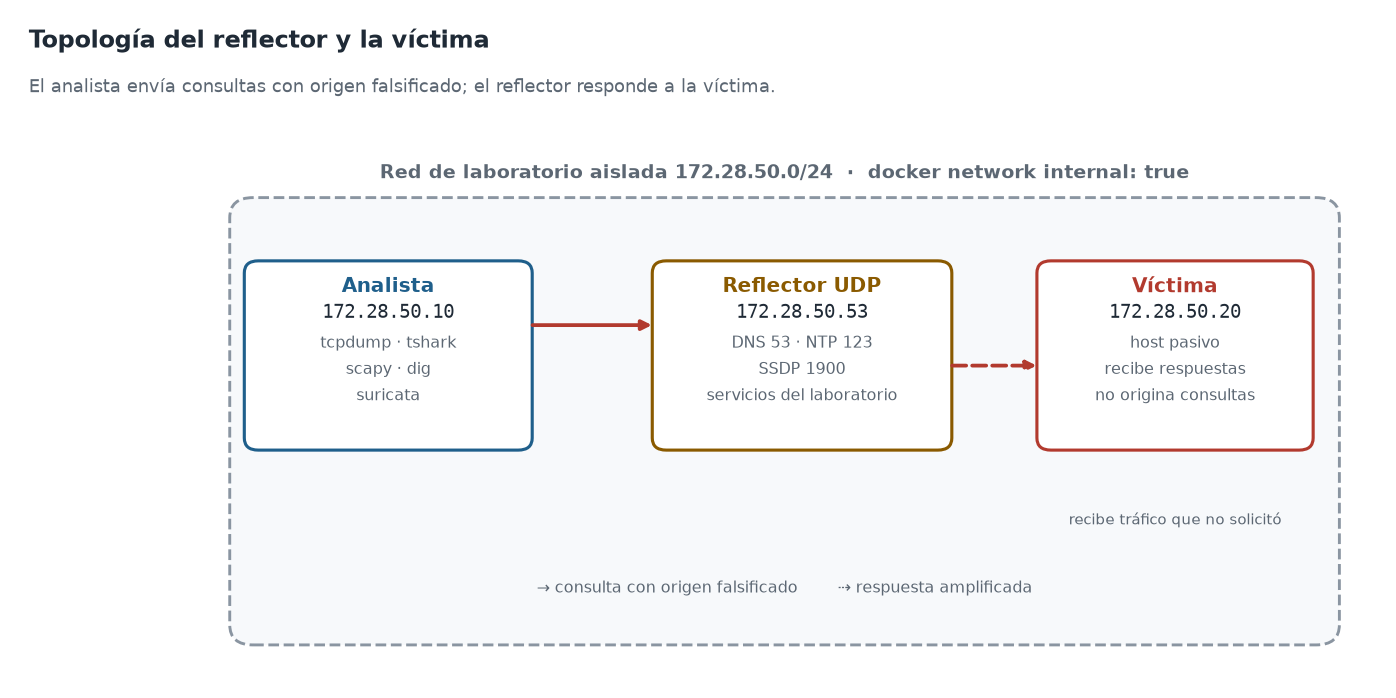
\includegraphics[width=0.95\textwidth]{imagenes/Evidencias CU-6/01_topologia_lab.png}
	\caption{Topología del reflector y la víctima en el Caso 6.}
	\label{fig:c6_topologia}
\end{figure}

\begin{figure}[H]
	\centering
	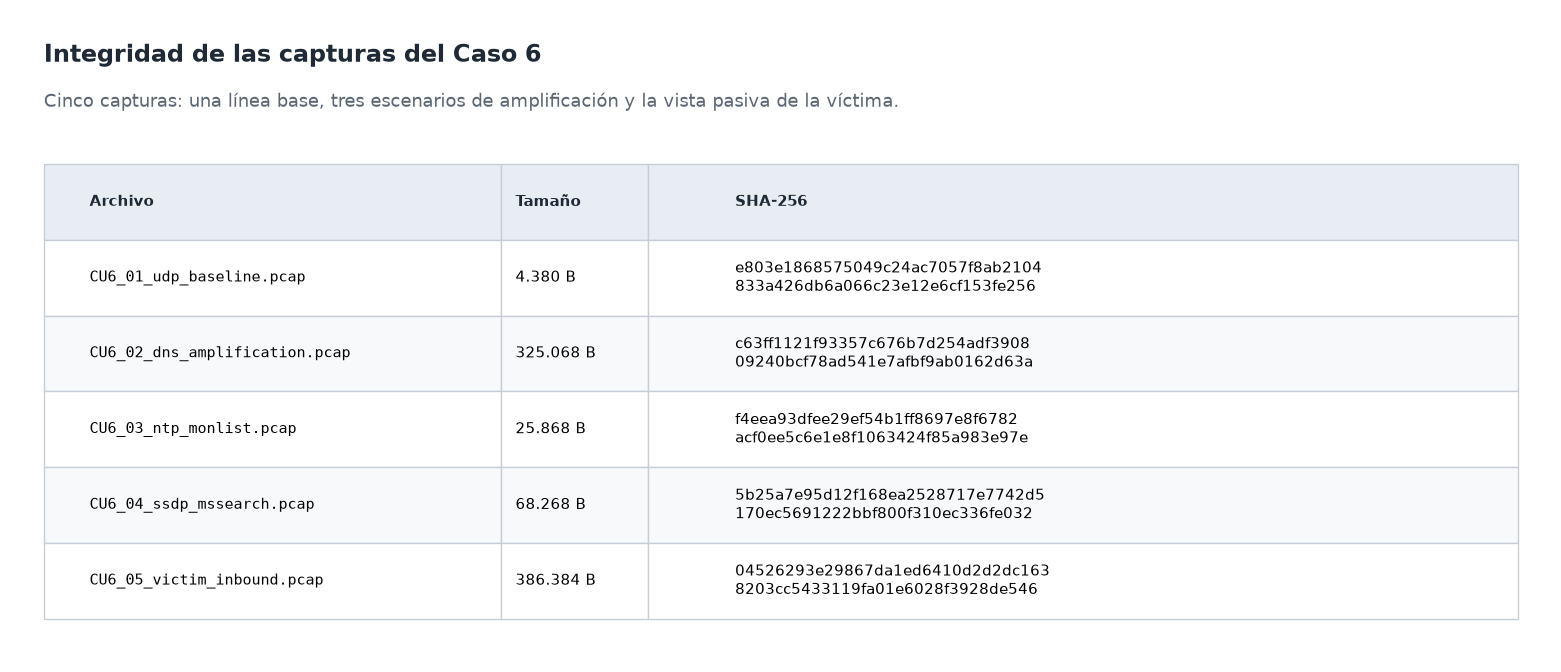
\includegraphics[width=0.92\textwidth]{imagenes/Evidencias CU-6/02_hashes_sha256.png}
	\caption{Verificación de integridad de las capturas del Caso 6 mediante SHA-256.}
	\label{fig:c6_hashes}
\end{figure}

\begin{figure}[H]
	\centering
	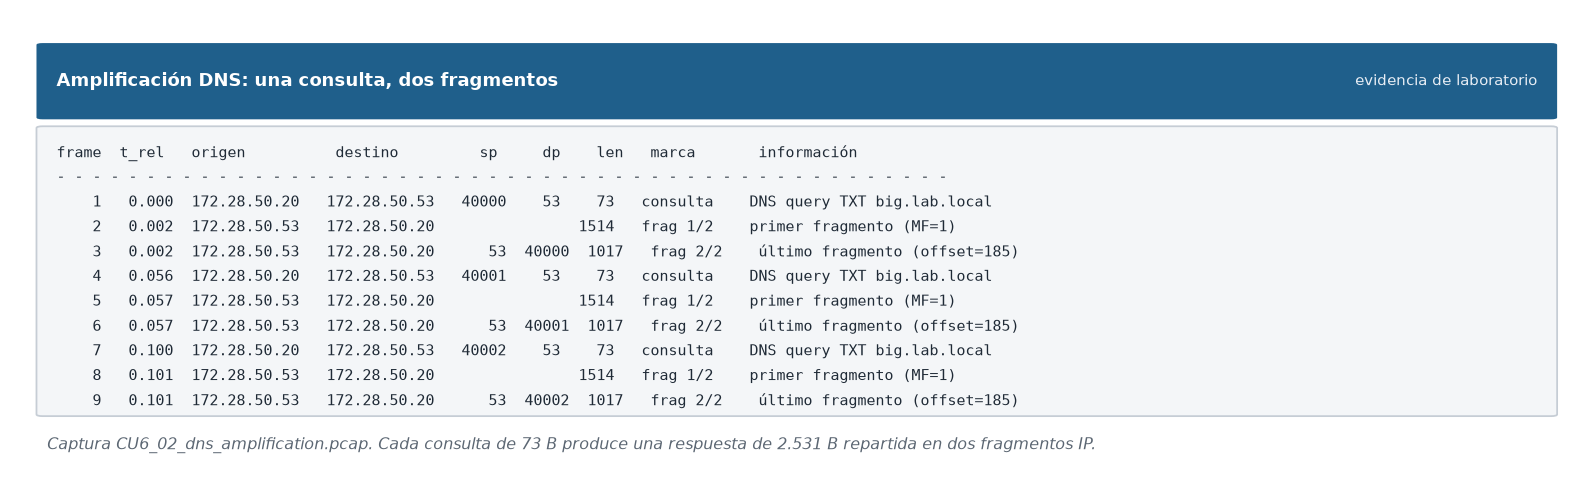
\includegraphics[width=0.98\textwidth]{imagenes/Evidencias CU-6/03_dns_amplificacion.png}
	\caption{Amplificación DNS: una consulta de 73~bytes y una respuesta de 2.531~bytes en dos fragmentos.}
	\label{fig:c6_dns}
\end{figure}

\paragraph{Resultados obtenidos.}
La Tabla~\ref{tab:c6_resumen} resume las cuatro fases medidas en el reflector. El factor de amplificación se calcula sobre los bytes de todas las tramas de respuesta divididos entre los bytes de todas las tramas de petición, incluidas las cabeceras Ethernet, IP y UDP; es, por tanto, una medida conservadora de lo que viaja por el enlace.

\begin{table}[H]
	\caption{Métricas de las capturas del Caso 6}
	\label{tab:c6_resumen}
	\centering
	\footnotesize
	\renewcommand{\arraystretch}{1.25}
	\begin{tabularx}{\textwidth}{@{}>{\raggedright\arraybackslash}p{0.18\textwidth} c c c c >{\raggedright\arraybackslash}p{0.18\textwidth} c@{}}
		\toprule
		\textbf{Escenario} & \textbf{Tramas} & \textbf{Bytes} & \textbf{Pet.} & \textbf{Resp.} & \textbf{Bytes pet.\ / resp.} & \textbf{Factor} \\
		\midrule
		Línea base & 27 & 3.344 & 12 & 15 & 956 / 2.388 & 2,5$\times$ \\
		DNS & 360 & 312.480 & 120 & 240 & 8.760 / 303.720 & 34,7$\times$ \\
		NTP monlist & 80 & 23.040 & 40 & 40 & 3.760 / 19.280 & 5,1$\times$ \\
		SSDP & 200 & 61.760 & 40 & 160 & 5.440 / 56.320 & 10,4$\times$ \\
		\bottomrule
	\end{tabularx}
\end{table}

\begin{itemize}
	\item \textbf{Línea base:} 27 tramas en 1,9~s. Las respuestas DNS son algo mayores que las consultas, de modo que el factor es 2,5$\times$ sin que exista un ataque. Esa asimetría normal es la razón por la que el factor, aislado, no basta.
	\item \textbf{DNS:} 120 consultas de 73~bytes generaron 120 respuestas de 2.531~bytes, todas fragmentadas en dos tramas (1.514 y 1.017~bytes). El volumen de respuesta fue de 303.720~bytes frente a 8.760~bytes de petición: 34,7$\times$ en el enlace. Si se cuenta solo la carga DNS, la relación es aún mayor (2.455~bytes de respuesta frente a 31~bytes de consulta), porque la consulta cabe en una trama y la respuesta ocupa dos.
	\item \textbf{NTP monlist:} 40 peticiones de 94~bytes (52~bytes de carga) y 40 respuestas de 482~bytes (440~bytes de carga). El factor en el enlace es 5,1$\times$; sobre la carga del protocolo es 8,5$\times$, el valor clásico de monlist.
	\item \textbf{SSDP:} 40 \texttt{M-SEARCH} de 136~bytes produjeron 160 respuestas de 352~bytes. El factor es 10,4$\times$ en el enlace y 13,2$\times$ sobre la carga, porque cada petición genera cuatro respuestas.
\end{itemize}

\begin{figure}[H]
	\centering
	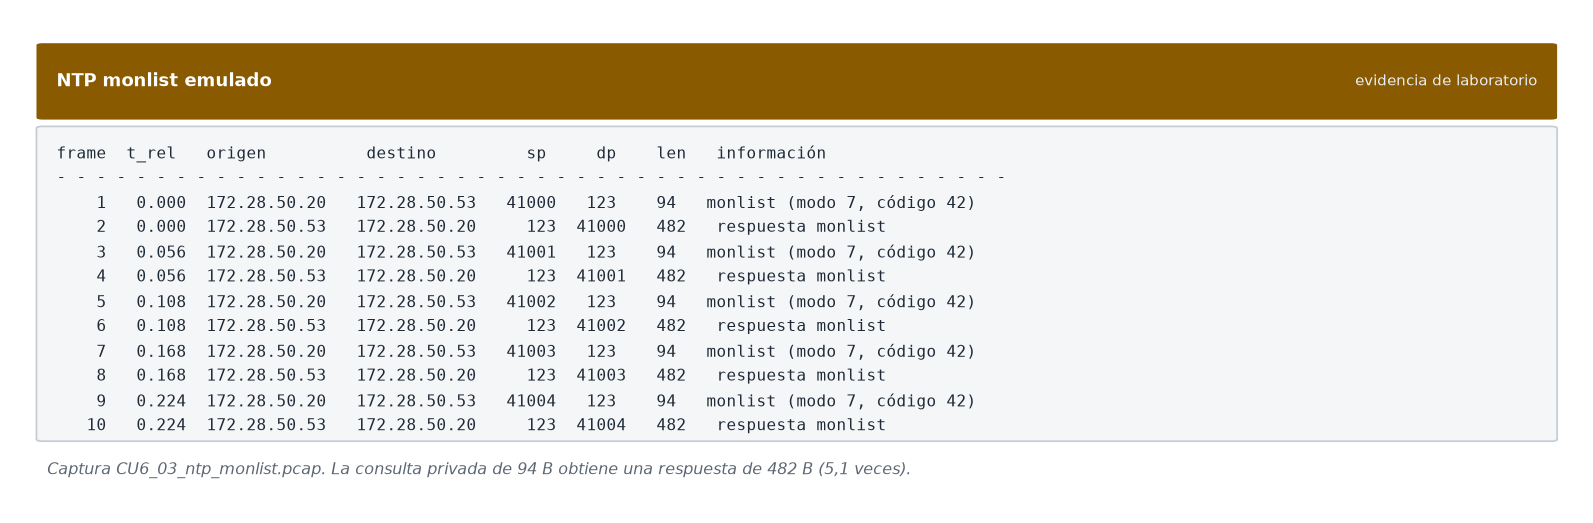
\includegraphics[width=0.98\textwidth]{imagenes/Evidencias CU-6/04_ntp_monlist.png}
	\caption{Consulta y respuesta NTP monlist emuladas (extracto de \texttt{CU6\_03\_ntp\_monlist.pcap}).}
	\label{fig:c6_ntp}
\end{figure}

\begin{figure}[H]
	\centering
	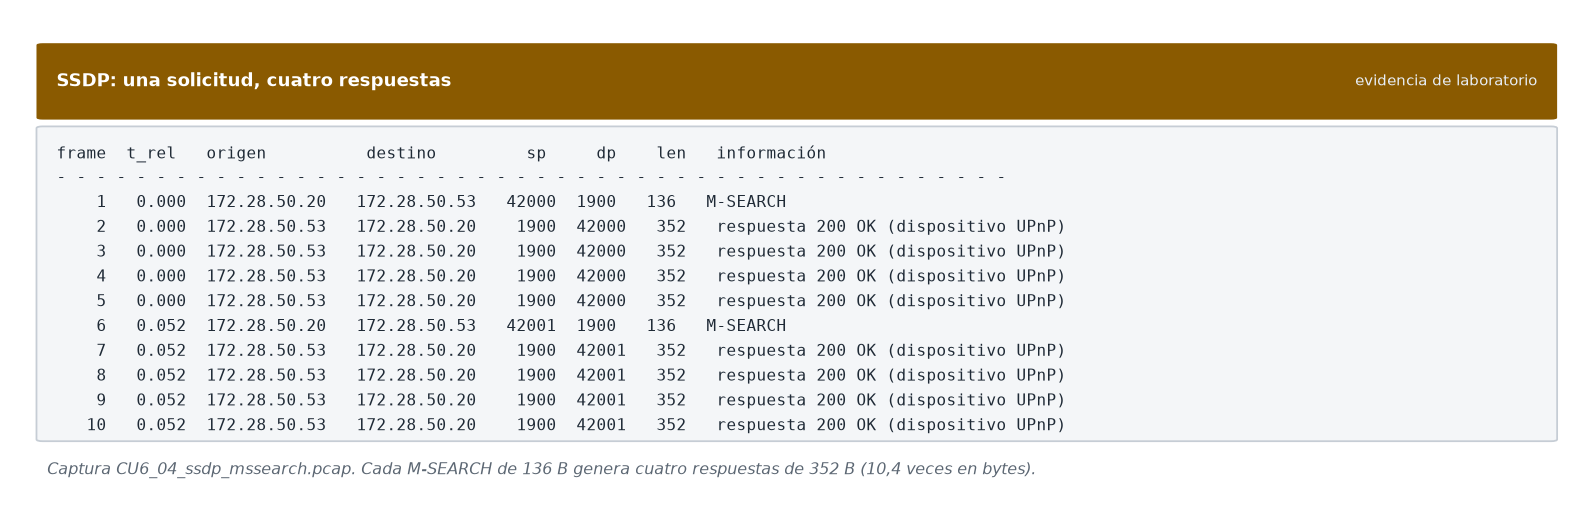
\includegraphics[width=0.98\textwidth]{imagenes/Evidencias CU-6/05_ssdp.png}
	\caption{Una solicitud SSDP y cuatro respuestas (extracto de \texttt{CU6\_04\_ssdp\_mssearch.pcap}).}
	\label{fig:c6_ssdp}
\end{figure}

\begin{figure}[H]
	\centering
	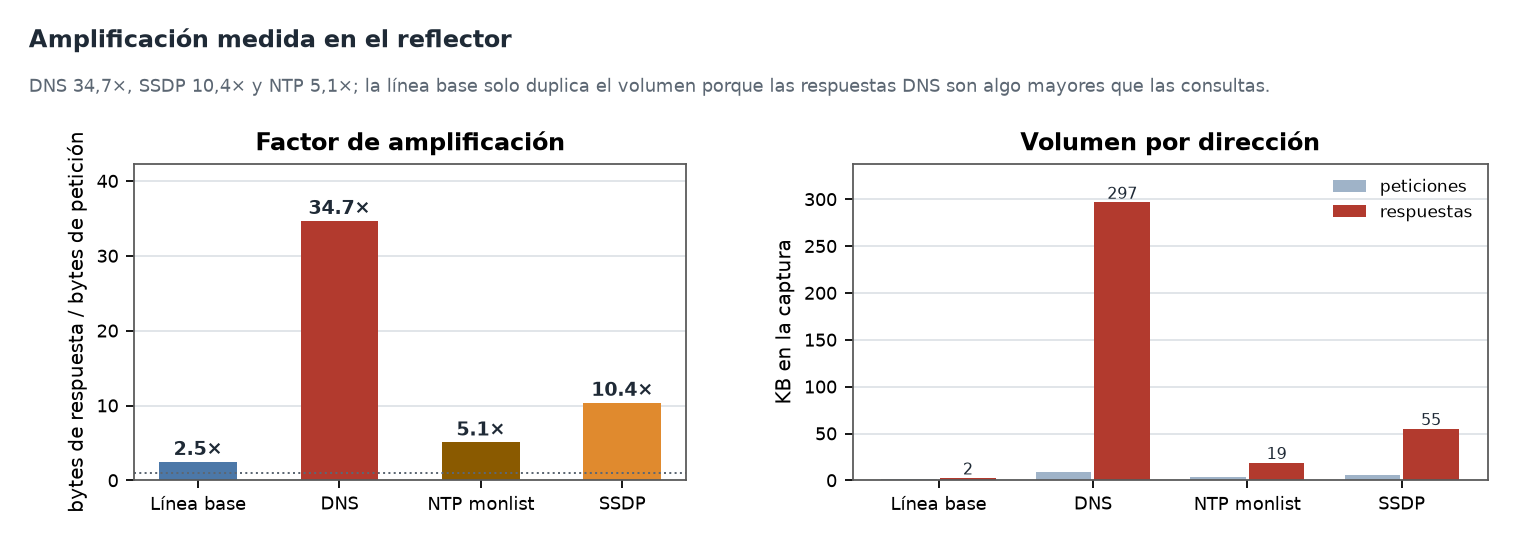
\includegraphics[width=0.96\textwidth]{imagenes/Evidencias CU-6/06_amplificacion.png}
	\caption{Factor de amplificación y volumen por dirección en cada escenario.}
	\label{fig:c6_factor}
\end{figure}

\paragraph{Análisis de resultados.}
La línea base demuestra que la asimetría entre petición y respuesta es normal en DNS: el servidor devuelve más de lo que recibe porque la respuesta incluye el nombre consultado y los registros. Por eso el factor de amplificación solo tiene sentido cuando se compara con el comportamiento esperado del mismo servicio y se acompaña de otra evidencia.

Esa segunda evidencia es la dirección. En la línea base, las respuestas vuelven al mismo host que consultó (\texttt{172.28.50.10}). En las tres fases de amplificación, las respuestas viajan a \texttt{172.28.50.20}, que no envió ninguna consulta. La captura de la víctima lo confirma: 440 tramas y 379.320~bytes recibidos en 11,7~s, con 120 respuestas DNS fragmentadas, 40 respuestas NTP y 160 respuestas SSDP, y cero consultas originadas por el host (Figura~\ref{fig:c6_victima}). La combinación de ambas capturas —reflector y víctima— es la que sostiene la conclusión; ninguna de las dos, por separado, prueba la falsificación del origen.

\begin{figure}[H]
	\centering
	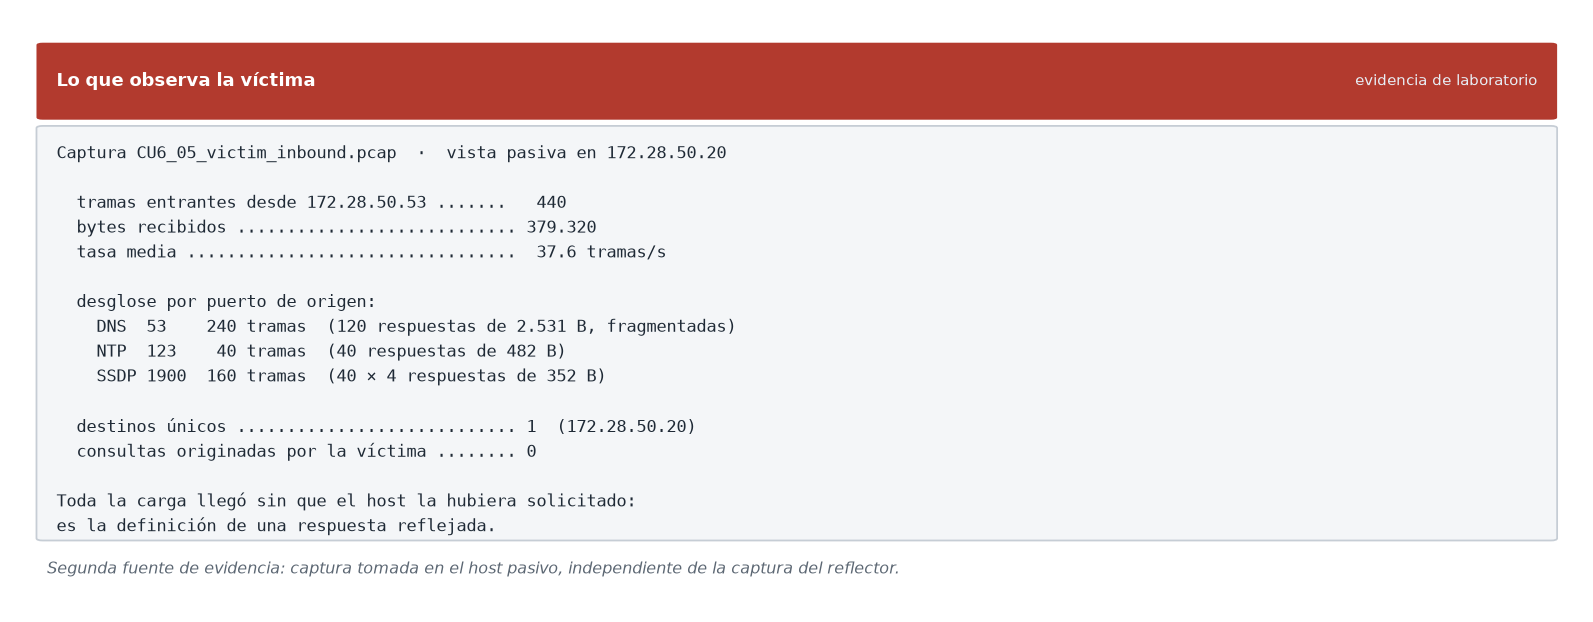
\includegraphics[width=0.98\textwidth]{imagenes/Evidencias CU-6/07_victima.png}
	\caption{Tráfico entrante observado en la víctima, que no originó ninguna consulta.}
	\label{fig:c6_victima}
\end{figure}

La fragmentación es un indicador adicional. Una respuesta DNS de 2.455~bytes no cabe en una trama de 1.500~bytes y se parte en dos; en la captura, las 240 tramas de respuesta corresponden a 120 respuestas fragmentadas. Un IDS que solo inspeccione la primera trama o que descarte fragmentos puede perder el evento, y un analista que cuente tramas en lugar de respuestas puede sobreestimar el número de mensajes. En este caso se reportan ambas cifras de forma explícita.

El tamaño del reflector importa. Los factores medidos dependen de la respuesta configurada: 2.455~bytes de carga DNS, 440~bytes de carga NTP y cuatro respuestas SSDP de 352~bytes en el enlace. En Internet, los factores publicados para DNS superan con frecuencia 30$\times$ y pueden llegar a 50$\times$ o más con respuestas DNSSEC o ANY \parencite{nawrocki2021farside}; los valores del laboratorio son coherentes con esa escala y no pretenden reproducir un ataque real de gran volumen.

\paragraph{Indicadores de detección.}
\begin{itemize}
	\item \textbf{Respuestas no solicitadas:} un host recibe respuestas DNS, NTP o SSDP sin consultas previas registradas.
	\item \textbf{Relación respuesta/petición:} volumen de respuesta muy superior al de petición para un mismo destino y protocolo, comparado con la línea base del servicio.
	\item \textbf{Fragmentación:} respuestas UDP grandes divididas en varios fragmentos IP.
	\item \textbf{NTP modo 7:} peticiones privadas con código 42 (monlist), que ningún cliente legítimo moderno necesita.
	\item \textbf{SSDP repetido:} ráfagas de \texttt{M-SEARCH} desde un mismo origen, cada una con varias respuestas.
	\item \textbf{Concentración de destinos:} muchas respuestas dirigidas a un mismo host y puertos de origen variados.
	\item \textbf{Asimetría de flujo:} el destino recibe mucho más de lo que envía y no tiene conexiones asociadas.
\end{itemize}

\paragraph{Regla de detección propuesta.}
Las reglas se validaron contra las cuatro capturas del reflector. La 1006001 detecta respuestas DNS grandes; la 1006002, la consulta monlist; la 1006003, la ráfaga de \texttt{M-SEARCH}.

\begin{verbatim}
alert udp any 53 -> any any (
  msg:"CU6 respuesta DNS de gran tamano (posible amplificacion)";
  dsize:>1000;
  threshold: type threshold, track by_dst, count 20, seconds 10;
  classtype:attempted-dos; sid:1006001; rev:1;)

alert udp any any -> any 123 (
  msg:"CU6 solicitud NTP monlist (modo 7)";
  content:"|17 00|"; depth:2; content:"|00 2a|"; offset:8; depth:2;
  classtype:attempted-dos; sid:1006002; rev:1;)

alert udp any any -> any 1900 (
  msg:"CU6 rafaga de M-SEARCH SSDP (posible reflexion)";
  content:"M-SEARCH"; depth:8;
  threshold: type threshold, track by_src, count 20, seconds 10;
  classtype:attempted-dos; sid:1006003; rev:1;)
\end{verbatim}

El reprocesamiento produjo cero alertas en la línea base, seis de la regla 1006001 en la fase DNS, cuarenta de la 1006002 en NTP y dos de la 1006003 en SSDP (Figura~\ref{fig:c6_suricata}). La regla 1006001 usa un umbral de veinte respuestas grandes por destino en diez segundos: una respuesta grande aislada no alerta, pero una ráfaga sí. La regla de frecuencia del Caso~2 también se activó en la fase DNS, lo que muestra que una misma señal puede pertenecer a dos casos: ciento veinte consultas en seis segundos son, a la vez, una ráfaga de DNS y el motor de una amplificación.

\begin{figure}[H]
	\centering
	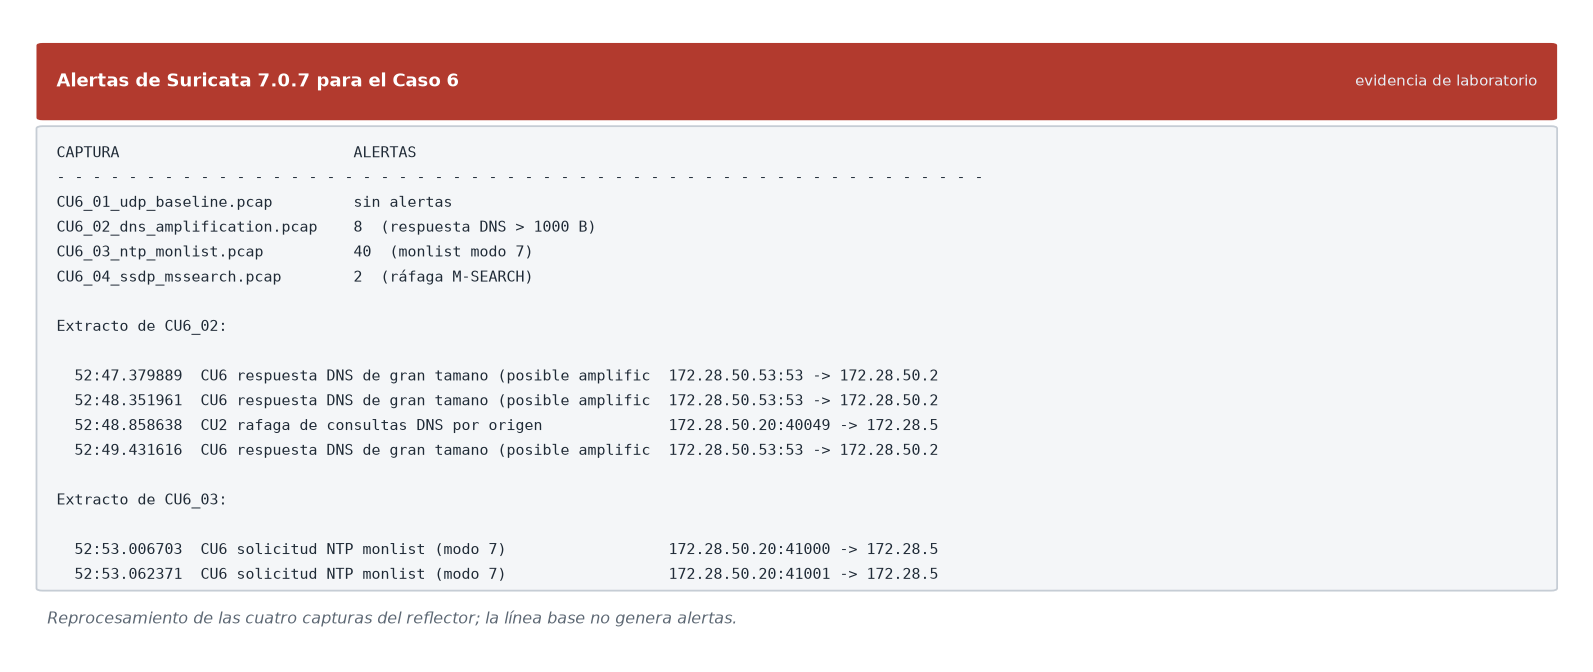
\includegraphics[width=0.98\textwidth]{imagenes/Evidencias CU-6/08_suricata_alertas.png}
	\caption{Alertas de Suricata 7.0.7 al reprocesar las capturas del Caso 6.}
	\label{fig:c6_suricata}
\end{figure}

\paragraph{Mitigación y defensa.}
\begin{itemize}
	\item \textbf{En el servidor:} deshabilitar la recursión abierta y permitirla solo a clientes autorizados; deshabilitar \textit{monlist} y los comandos privados de NTP; restringir SSDP a la red local; aplicar limitación de tasa de respuestas (RRL) y límites de tamaño; apagar los servicios que no se usan.
	\item \textbf{En la red del operador:} filtrado de origen (BCP~38) y unicast reverse path forwarding en el borde; ACL de puertos UDP sensibles; telemetría de flujos para detectar picos por destino; mitigación con \textit{scrubbing} o limitación en el peering.
	\item \textbf{En la red de la víctima:} filtrado de entrada para descartar respuestas no solicitadas y limitación de tasa por destino; sirve para contener el daño, pero no elimina la causa.
	\item \textbf{En la operación:} inventario de servicios UDP expuestos, revisión periódica de configuraciones, pruebas de reflexión solo en laboratorio y coordinación con el proveedor ante un evento sostenido.
	\item \textbf{En la detección:} combinar el tamaño de la respuesta con la ausencia de consulta previa y con la dirección del flujo; una regla de tamaño aislada puede confundir una respuesta DNS legítima grande con un ataque.
\end{itemize}
La causa raíz —la falsificación de origen— solo se corrige en la red que origina el tráfico, que casi nunca es la de la víctima. Por eso los controles se reparten entre el operador del servicio, el proveedor de tránsito y la red de destino.

\paragraph{Preguntas de análisis.}
\begin{enumerate}
	\item \textbf{¿Cómo se diferencia una ráfaga legítima de un patrón de reflexión?}\par
	Por la correlación con la solicitud. En una ráfaga legítima, el host que recibe la respuesta es el mismo que envió la consulta y existe un registro de esa consulta en el cliente o en el resolver; en una reflexión, el destino no envió nada y el origen aparente es una dirección falsificada. Ayudan también el tamaño y la fragmentación de la respuesta, la cantidad de respuestas por petición, la variedad de puertos de origen, la duración y la comparación con la línea base del servicio. En este laboratorio, la prueba decisiva fue la captura de la víctima con cero consultas originadas.
	\item \textbf{¿Qué controles corresponden al servidor y cuáles al proveedor de red?}\par
	Al servidor le corresponden la configuración y el uso: cerrar la recursión, deshabilitar \textit{monlist}, limitar SSDP, aplicar RRL y límites de tamaño. Al proveedor de red le corresponden el filtrado anti-\textit{spoofing} en el origen, la telemetría, la limitación en el peering y la mitigación del volumen. La víctima solo puede filtrar lo que recibe. Ningún control aislado resuelve el problema: sin filtrado de origen, el atacante puede seguir usando cualquier reflector abierto.
\end{enumerate}

\paragraph{Conclusiones.}
\begin{itemize}
	\item Se midió la amplificación de tres protocolos en un entorno aislado: DNS 34,7$\times$, SSDP 10,4$\times$ y NTP 5,1$\times$ en bytes de enlace, con factores sobre la carga de 79$\times$, 13,2$\times$ y 8,5$\times$ respectivamente.
	\item La línea base mostró una asimetría normal de 2,5$\times$: la asimetría por sí sola no es un indicador de ataque.
	\item La captura de la víctima, independiente de la del reflector, confirmó 379.320~bytes entrantes y cero consultas originadas.
	\item La fragmentación de las respuestas DNS fue un indicador visible y, a la vez, una dificultad de conteo que el análisis debió resolver.
	\item Las reglas 1006001, 1006002 y 1006003 detectaron los tres escenarios sin alertar en la línea base; la regla de frecuencia del Caso~2 también se activó, lo que evidencia el cruce entre casos.
	\item Limitaciones: los servicios de NTP y SSDP son emulaciones didácticas, el reflector se configuró deliberadamente abierto, la escala es pequeña y no se reproduce un ataque distribuido ni una red real de terceros.
\end{itemize}

\begin{table}[H]
	\centering
	\caption{Ficha de registro del hallazgo. Caso 6}
	\footnotesize
	\renewcommand{\arraystretch}{1.2}
	\begin{tabularx}{\textwidth}{@{}>{\raggedright\arraybackslash}p{0.23\textwidth} Y@{}}
		\toprule
		\textbf{Campo} & \textbf{Registro} \\ \midrule
		Identificador & Caso 6 (reflexión/amplificación UDP), evidencias \texttt{01\_topologia\_lab.png} a \texttt{08\_suricata\_alertas.png}. Analista: equipo de laboratorio. \\ \hline
		Fecha y hora & 10 de noviembre de 2026, 16:52 (UTC$-$5); \texttt{CU6\_01} a \texttt{CU6\_05}. \\ \hline
		Origen/destino & Origen falsificado \texttt{172.28.50.20}, reflector \texttt{172.28.50.53}, puertos UDP 53, 123 y 1900. \\ \hline
		Observación & 120 consultas DNS, 40 consultas monlist y 40 \texttt{M-SEARCH} con origen falsificado; respuestas de 2.531, 482 y 4~$\times$~352~bytes, respectivamente. \\ \hline
		Hipótesis & La amplificación se reconocerá por una relación respuesta/petición superior a la línea base y por respuestas que llegan a un host que no consultó. \\ \hline
		Validación & Captura del reflector y captura independiente de la víctima: 379.320~bytes entrantes y cero consultas originadas. Suricata: 0, 6, 40 y 2 alertas. \\ \hline
		Severidad & Alta en producción por el volumen y la facilidad de repetición; informativa en el laboratorio aislado. \\ \hline
		Acción & Cerrar la recursión, deshabilitar monlist, restringir SSDP, aplicar RRL y filtrado de origen, y monitorear flujos por destino. \\ \hline
		Integridad & \texttt{CU6\_02}: \texttt{c63ff112\dots0162d63a}; \texttt{CU6\_05}: \texttt{04526293\dots928de546} (SHA-256 truncado; el valor completo está en el Anexo~A). \\
		\bottomrule
	\end{tabularx}
\end{table}

\subsection{Caso 7. ICMP: escaneo, payloads atípicos y posible túnel}
\label{caso:icmp}

\begin{situacion}
Se observa una tasa de ICMP mayor de lo habitual o paquetes con tamaños o patrones repetitivos. ICMP se especifica en el RFC~792 \parencite{rfc792}.
\end{situacion}

\paragraph{Procedimiento.}
\begin{itemize}[leftmargin=*, topsep=2pt, itemsep=2pt]
	\item En Wireshark, filtrar \texttt{icmp} y agrupar por IP de origen/destino, tipo, código, longitud y tiempo.
	\item Establecer una línea base de ping de diagnóstico legítimo y compararla con la captura analizada.
	\item Usar PCAP sintético o didáctico para estudiar payloads; no transmitir información sensible por ICMP.
\end{itemize}

\paragraph{Indicadores que deben buscarse.}
Ráfagas de echo request/reply, longitudes inusuales, periodicidad repetitiva o volumen no explicado por tareas de diagnóstico.

\paragraph{Mitigación y defensa.}
Permitir solo los tipos ICMP necesarios para la operación y el diagnóstico; aplicar límites proporcionados; monitorizar sin bloquear indiscriminadamente mensajes requeridos por la red.

\paragraph{Evidencias que se entregan.}
Dashboard por IP, filtro aplicado, tabla de tamaños y frecuencias, y propuesta de regla.

\paragraph{Preguntas de análisis.}
\begin{enumerate}[leftmargin=*, topsep=2pt, itemsep=2pt]
	\item ¿Qué funciones legítimas cumple ICMP?
	\item ¿Qué impacto tendría bloquearlo completamente?
\end{enumerate}

\begin{table}[H]
	\caption{Distribución de tráfico ICMP por tipo y longitud}
	\label{tab:icmp}
	\centering
	\footnotesize
	\renewcommand{\arraystretch}{1.25}
	\begin{tabularx}{\textwidth}{@{}c c c >{\raggedright\arraybackslash}p{0.17\textwidth} >{\raggedright\arraybackslash}p{0.17\textwidth} Y@{}}
		\toprule
		\textbf{Tipo} & \textbf{Código} & \textbf{Longitud} & \textbf{Origen} & \textbf{Destino} & \textbf{Frecuencia / observación} \\
		\midrule
		& & & & & \\
		& & & & & \\
		& & & & & \\
		& & & & & \\
		& & & & & \\
		\bottomrule
	\end{tabularx}
\end{table}

\registrohallazgo{Caso 7}

\subsection{Caso 8. Escaneo de puertos y fingerprinting de servicios}
\label{caso:escaneo-puertos}

\begin{situacion}
Los registros muestran intentos secuenciales contra varios puertos o servicios no habituales de un servidor de laboratorio.
\textbf{Objetivo:} \par
Reproducir un escaneo de puertos autorizado, medir su huella en la red y en un IDS, identificar los servicios expuestos y proponer una lista de exposición con controles de reducción de superficie y reglas de detección. \par
\textbf{Fundamento teórico:} \par
El escaneo de puertos aprovecha el comportamiento de TCP y UDP para inferir qué servicios escucha un host. En TCP, un escaneo SYN envía un segmento con la bandera SYN: si el puerto está abierto, el servidor responde SYN-ACK; si está cerrado, responde RST. El escaneo no completa el \textit{three-way handshake}, por lo que también se denomina \textit{half-open}. En UDP no existe un handshake equivalente: un puerto cerrado suele responder con ICMP de puerto inalcanzable, mientras que uno abierto puede no responder, lo que produce el estado ambiguo \texttt{open|filtered}. El \textit{fingerprinting} posterior envía sondas específicas por servicio para obtener banners y versiones \parencite{nmap}.
\end{situacion}

\paragraph{Procedimiento.}
El escenario reutiliza la red aislada del Caso 7: analista en \texttt{172.28.50.10} y víctima en \texttt{172.28.50.20}, con servicios FTP, SSH, Telnet, HTTP y dos servicios de prueba. El procedimiento fue:

\begin{enumerate}
	\raggedright
	\item \textbf{Integridad:} se calcularon las huellas SHA-256 de las tres capturas antes de analizarlas (Figura~\ref{fig:c8_hashes}).
	\item \textbf{Escaneo SYN:} se ejecutó \texttt{nmap -sS -Pn -n -p 1-1024 --min-rate 1500 --max-retries 1} y se capturó \texttt{CU8\_01\_syn\_scan.pcap} (Figura~\ref{fig:c8_nmap_syn}).
	\item \textbf{Fingerprinting:} se ejecutó \texttt{nmap -sT -sV -Pn -n -p 21,22,23,80,4444,8080 --version-all} y se capturó \texttt{CU8\_02\_service\_scan.pcap} (Figura~\ref{fig:c8_nmap_svc}).
	\item \textbf{Escaneo UDP:} se ejecutó \texttt{nmap -sU -Pn -n -p 53,123,161,500,5353} y se capturó \texttt{CU8\_03\_udp\_scan.pcap}.
	\item \textbf{Análisis de flujos:} con \texttt{tshark} se contaron paquetes SYN, SYN-ACK y RST, puertos destino únicos, duración y tasa (Figuras~\ref{fig:c8_cobertura} y~\ref{fig:c8_flags}).
	\item \textbf{Validación con IDS:} se reprocesó la captura SYN con Suricata 7.0.7 y las reglas locales (Figura~\ref{fig:c8_suricata}).
\end{enumerate}

\begin{figure}[H]
	\centering
	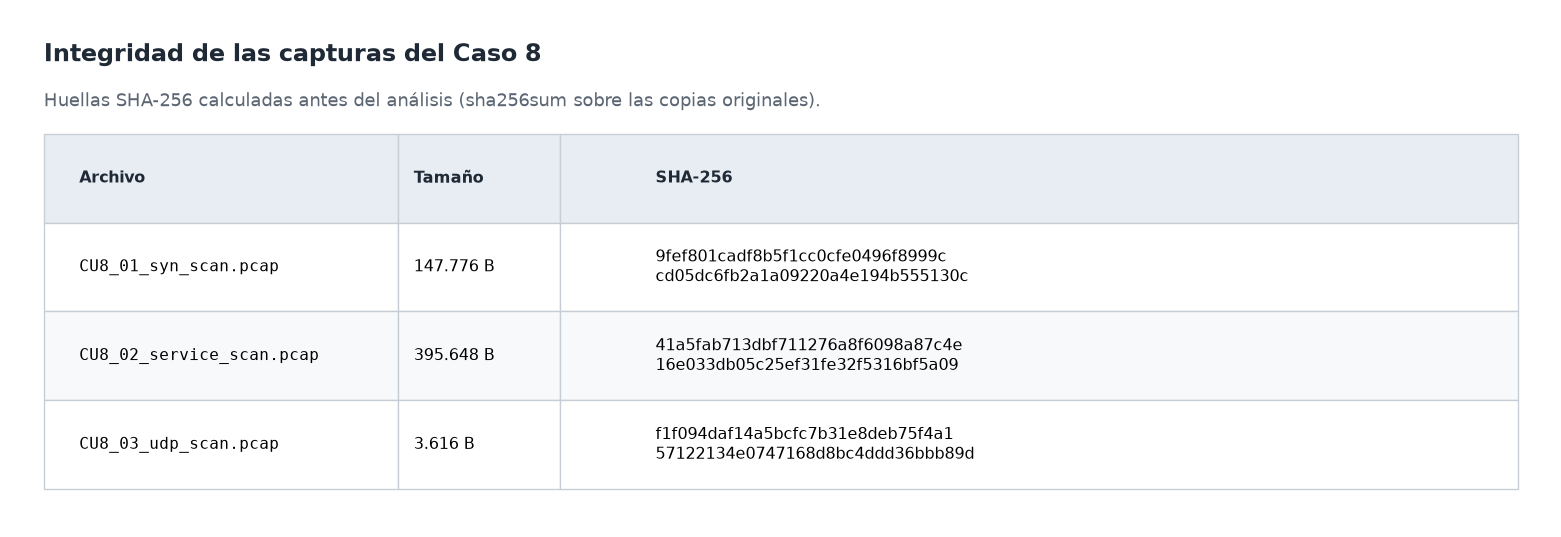
\includegraphics[width=0.92\textwidth]{imagenes/Evidencias CU-8/01_hashes_sha256.png}
	\caption{Verificación de integridad de las capturas del Caso 8 mediante SHA-256.}
	\label{fig:c8_hashes}
\end{figure}

\begin{figure}[H]
	\centering
	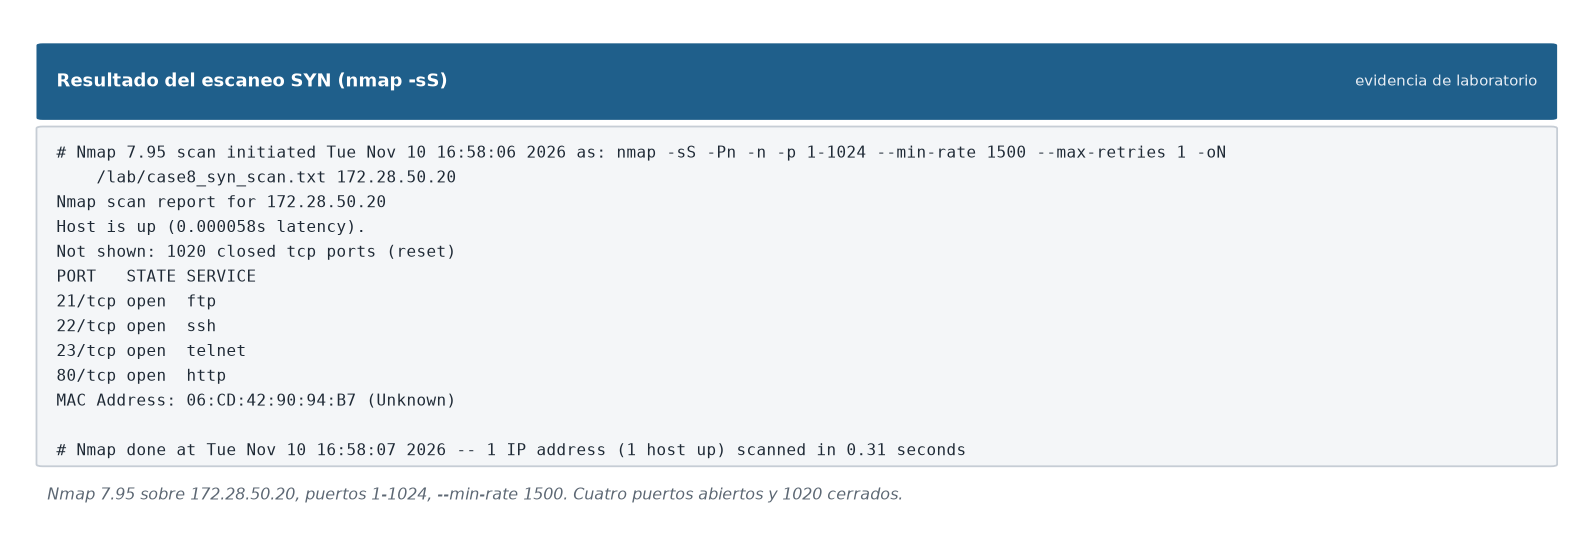
\includegraphics[width=0.98\textwidth]{imagenes/Evidencias CU-8/02_nmap_syn.png}
	\caption{Resultado del escaneo SYN sobre los puertos 1--1024 de la víctima.}
	\label{fig:c8_nmap_syn}
\end{figure}

\begin{figure}[H]
	\centering
	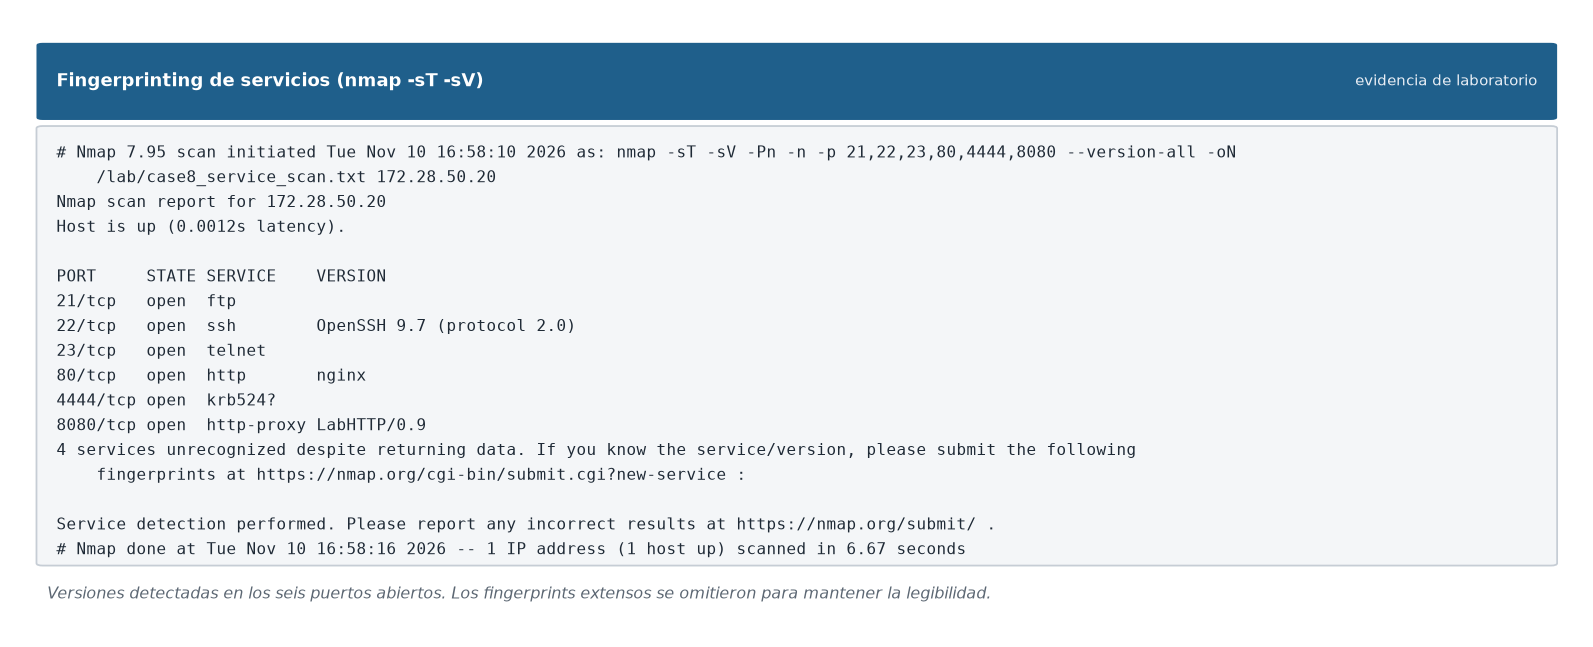
\includegraphics[width=0.98\textwidth]{imagenes/Evidencias CU-8/03_nmap_servicios.png}
	\caption{Detección de versiones y banners de los servicios expuestos.}
	\label{fig:c8_nmap_svc}
\end{figure}

\paragraph{Resultados obtenidos.}
La Tabla~\ref{tab:c8_resumen} resume las métricas de las tres capturas. El escaneo SYN generó 2052 paquetes TCP en 59~ms, con 1024 SYN, 4 SYN-ACK y 1020 RST; es decir, 1024 puertos únicos, de los cuales solo cuatro estaban abiertos (21, 22, 23 y 80). La tasa media fue de aproximadamente 17\,400 SYN por segundo (34\,817 paquetes TCP por segundo si se cuentan también las respuestas).

\begin{table}[H]
	\caption{Métricas de las capturas del Caso 8}
	\label{tab:c8_resumen}
	\centering
	\footnotesize
	\renewcommand{\arraystretch}{1.25}
	\begin{tabularx}{\textwidth}{@{}>{\raggedright\arraybackslash}p{0.26\textwidth} c c c Y@{}}
		\toprule
		\textbf{Captura} & \textbf{Paquetes} & \textbf{Puertos} & \textbf{Duración} & \textbf{Observación} \\ \midrule
		\texttt{CU8\_01\_syn\_scan} & 2052 TCP & 1024 & 59~ms & 1024 SYN, 4 SYN-ACK, 1020 RST. \\ \hline
		\texttt{CU8\_02\_service\_scan} & 4214 TCP & 6 & 6,67~s & 328\,200 bytes; banners y versiones. \\ \hline
		\texttt{CU8\_03\_udp\_scan} & 28 UDP & 5 & 1,75~s & 7 ICMP de puerto inalcanzable. \\
		\bottomrule
	\end{tabularx}
\end{table}

\begin{figure}[H]
	\centering
	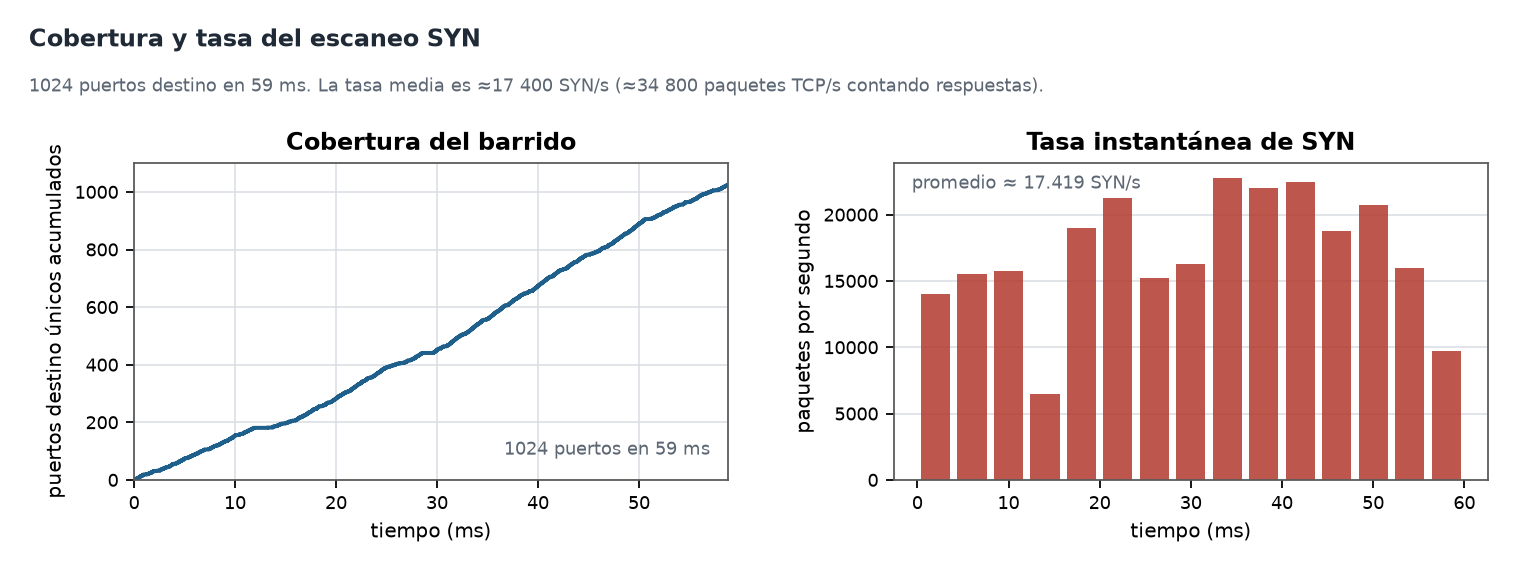
\includegraphics[width=0.98\textwidth]{imagenes/Evidencias CU-8/04_puertos_acumulados.png}
	\caption{Cobertura acumulada de puertos y tasa instantánea del escaneo SYN.}
	\label{fig:c8_cobertura}
\end{figure}

\begin{figure}[H]
	\centering
	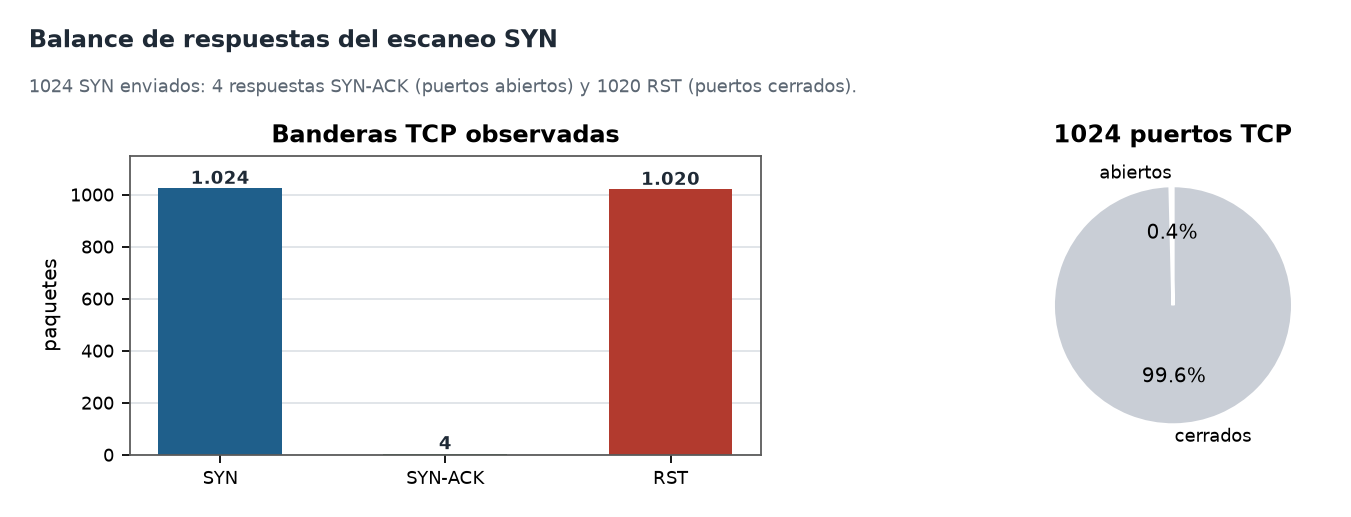
\includegraphics[width=0.92\textwidth]{imagenes/Evidencias CU-8/05_conteo_flags.png}
	\caption{Balance de banderas TCP y proporción de puertos abiertos frente a cerrados.}
	\label{fig:c8_flags}
\end{figure}

\paragraph{Análisis de resultados.}
El escaneo SYN deja una huella muy reconocible: una ráfaga de segmentos SYN con puertos destino crecientes, seguida de RST para los puertos cerrados y de SYN-ACK para los abiertos. La proporción de RST (1020 de 1024 puertos, 99,6\,\%) y la ausencia de un handshake completo confirman el carácter \textit{half-open} del barrido. La tasa instantánea, superior a 20\,000 SYN/s en varios intervalos, es muy superior a la de un cliente legítimo y explica por qué un umbral simple de 30 SYN en 10~s detecta el evento.

El escaneo de servicios, en cambio, sí completa conexiones y solicita banners. Eso permite identificar versiones concretas: OpenSSH~9.7 en el puerto 22, nginx en el 80, \texttt{Laboratorio FTP 1.0} en el 21, \texttt{Laboratorio Telnet 0.9} en el 23 y \texttt{LabHTTP/0.9} en el 8080. El puerto 4444 respondió con \texttt{LAB-SVC/0.1 ready}, un servicio no estándar que Nmap no pudo clasificar y etiquetó como \texttt{krb524?}; esa ambigüedad es una limitación del fingerprinting y, a la vez, una señal de que el servicio no debería estar expuesto sin justificación.

El escaneo UDP fue mucho menos concluyente: 53, 123, 161 y 5353 respondieron con ICMP de puerto inalcanzable (cerrados), mientras que el 500 quedó en \texttt{open|filtered} porque no hubo respuesta. La ausencia de respuesta no prueba que el puerto esté abierto: puede deberse a un filtrado silencioso.

\begin{figure}[H]
	\centering
	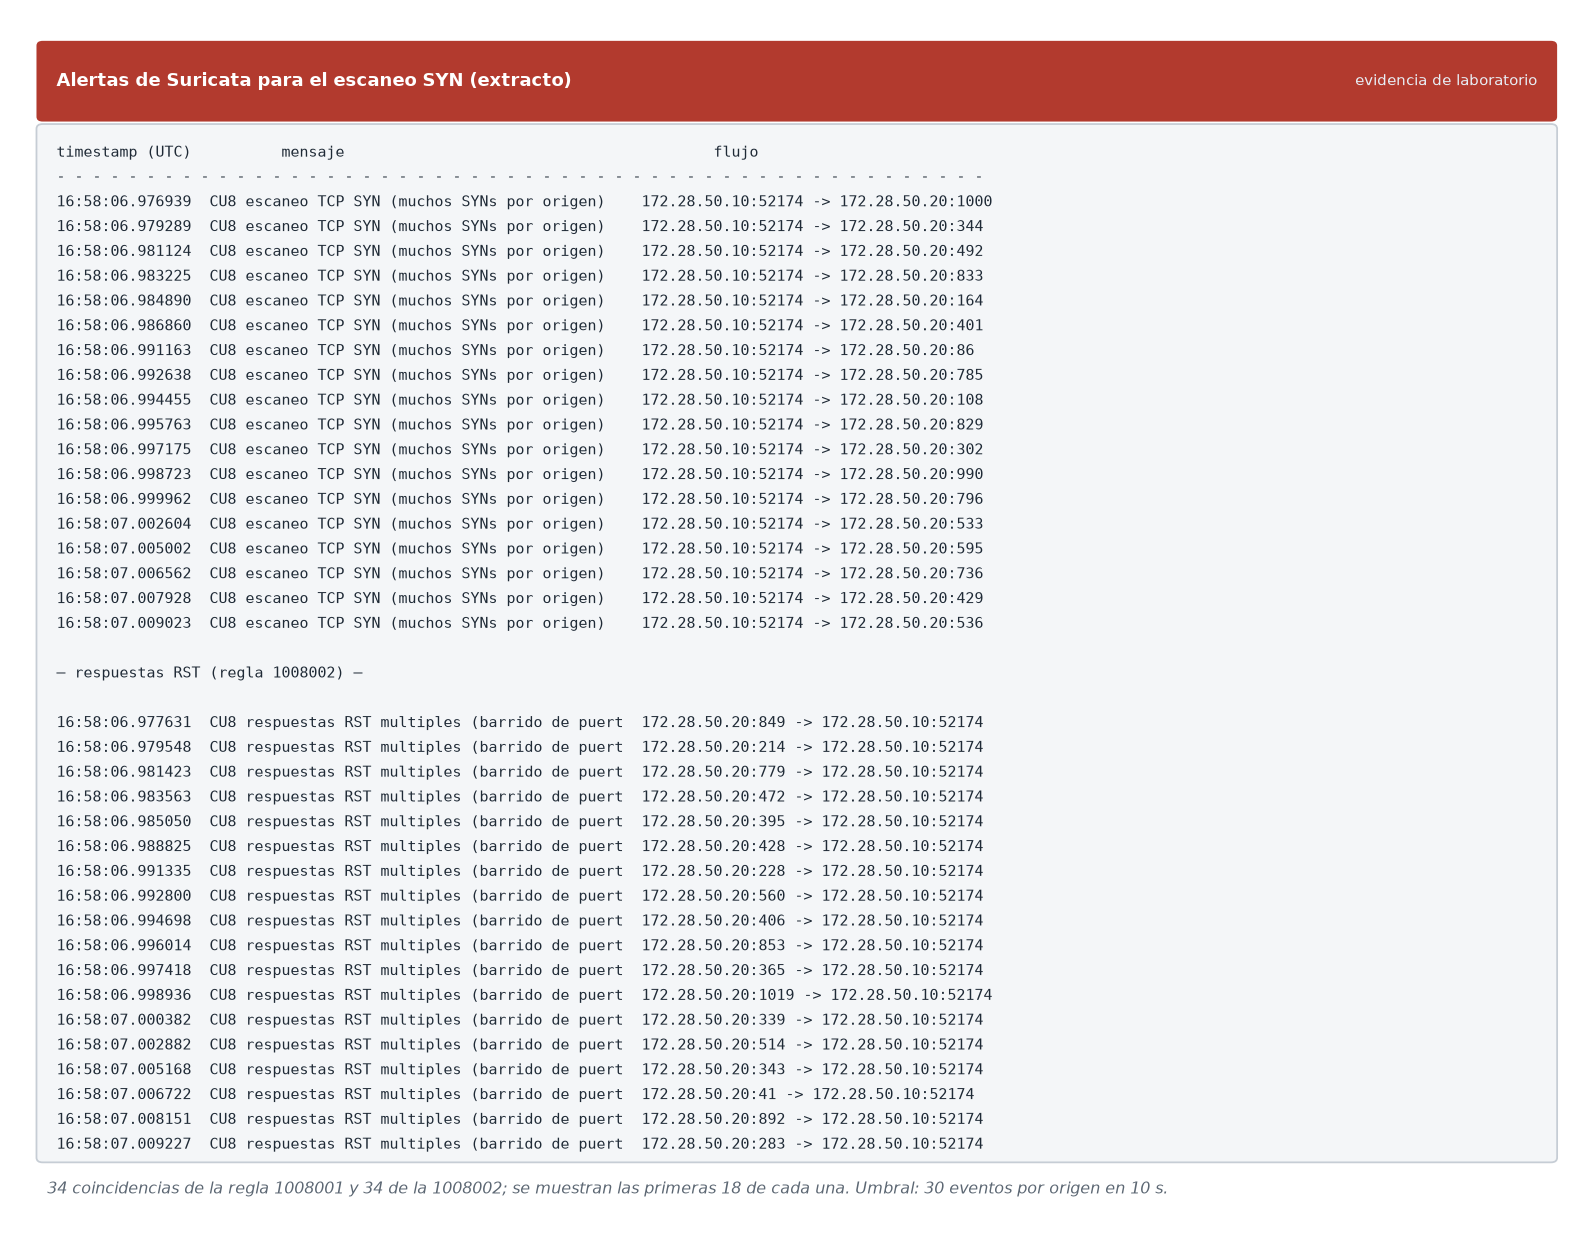
\includegraphics[width=0.98\textwidth]{imagenes/Evidencias CU-8/06_suricata_alertas.png}
	\caption{Alertas de Suricata 7.0.7 para el escaneo SYN (extracto de \texttt{fast.log}).}
	\label{fig:c8_suricata}
\end{figure}

\paragraph{Indicadores de detección.}
\begin{itemize}
	\item \textbf{Ráfaga de SYN:} más de 30 segmentos SYN desde un mismo origen en 10~s.
	\item \textbf{Barrido de puertos:} muchos puertos destino únicos y crecientes en un intervalo corto.
	\item \textbf{Relación SYN/RST:} predominio de RST sobre SYN-ACK, señal de puertos cerrados.
	\item \textbf{Fingerprinting:} conexiones completas seguidas de banners o cadenas de versión en varios puertos.
	\item \textbf{UDP e ICMP:} ráfaga de datagramas UDP con respuestas ICMP de puerto inalcanzable.
\end{itemize}

\paragraph{Regla de detección propuesta.}
Las reglas se validaron con Suricata: 34 alertas de la regla~1008001 y 34 de la regla~1008002 sobre \texttt{CU8\_01\_syn\_scan.pcap}. El umbral de 30 eventos por origen en 10~s evita que un cliente que abre varias conexiones normales dispare la alerta.

\begin{verbatim}
alert tcp 172.28.50.10 any -> 172.28.50.20 any (
  msg:"CU8 escaneo TCP SYN (muchos SYNs por origen)"; flags:S;
  threshold:type threshold, track by_src, count 30, seconds 10;
  classtype:attempted-recon; sid:1008001; rev:1;)

alert tcp 172.28.50.20 any -> 172.28.50.10 any (
  msg:"CU8 respuestas RST multiples (barrido de puertos)"; flags:R*;
  threshold:type threshold, track by_dst, count 30, seconds 10;
  classtype:attempted-recon; sid:1008002; rev:1;)
\end{verbatim}

\paragraph{Lista de exposición y endurecimiento.}
La Tabla~\ref{tab:exposicion} clasifica los servicios observados. La decisión de exposición debe justificarse por necesidad operativa y no por comodidad de instalación.

\begin{table}[H]
	\caption{Lista de exposición de servicios propios}
	\label{tab:exposicion}
	\centering
	\footnotesize
	\renewcommand{\arraystretch}{1.25}
	\begin{tabularx}{\textwidth}{@{}c >{\raggedright\arraybackslash}p{0.13\textwidth} >{\raggedright\arraybackslash}p{0.14\textwidth} c Y >{\raggedright\arraybackslash}p{0.18\textwidth}@{}}
		\toprule
		\textbf{Puerto} & \textbf{Servicio} & \textbf{Versión} & \textbf{¿Expuesto?} & \textbf{Justificación} & \textbf{Control propuesto} \\ \midrule
		21 & FTP & Laboratorio FTP 1.0 & Sí & Protocolo heredado sin cifrado. & Deshabilitar o migrar a SFTP/FTPS. \\ \hline
		22 & SSH & OpenSSH 9.7 & Sí & Administración remota. & Restringir por origen, solo claves y MFA. \\ \hline
		23 & Telnet & Laboratorio Telnet 0.9 & Sí & Credenciales en claro. & Deshabilitar de forma definitiva. \\ \hline
		80 & HTTP & nginx & Sí & Publicación web. & Redirigir a HTTPS y aplicar WAF. \\ \hline
		4444 & Desconocido & LAB-SVC/0.1 & Sí & Servicio de prueba sin justificación. & Cerrar salvo necesidad documentada. \\ \hline
		8080 & HTTP & LabHTTP/0.9 & Sí & Servicio de pruebas. & Restringir a la red de laboratorio. \\
		\bottomrule
	\end{tabularx}
\end{table}

\paragraph{Mitigación y defensa.}
\begin{itemize}
	\item \textbf{Reducción de superficie:} apagar servicios que no se usan y sustituir FTP/Telnet por SFTP/SSH.
	\item \textbf{Segmentación y firewall:} política de denegación por defecto y apertura solo desde redes y usuarios autorizados.
	\item \textbf{Control de tasa y bloqueo temporal:} limitar conexiones por origen y aplicar bloqueo con revisión ante barridos sostenidos.
	\item \textbf{Endurecimiento:} minimizar banners, actualizar versiones, usar TLS en los servicios publicados y revisar privilegios.
	\item \textbf{Monitorización:} correlacionar alertas de IDS con inventario de servicios y con ventanas de mantenimiento.
	\item \textbf{Pruebas autorizadas:} programar escaneos desde direcciones conocidas y documentarlos para separar el monitoreo legítimo de un ataque.
\end{itemize}

\paragraph{Preguntas de análisis.}
\begin{enumerate}
	\item \textbf{¿Qué limitaciones tiene atribuir un escaneo a una sola IP?}\par
	Una dirección IP no identifica de forma única a una persona o equipo: puede estar detrás de NAT o de un proxy, puede haber sido asignada por DHCP a otro host, puede estar suplantada mediante \textit{spoofing} o formar parte de una botnet distribuida. La atribución requiere correlacionar flujos, horarios, registros de autenticación, inventario de activos y, cuando exista, evidencia del proveedor; la IP por sí sola es solo un punto de partida.
	\item \textbf{¿Cómo se reducen los falsos positivos por monitoreo autorizado?}\par
	Con listas de escáneres autorizados, ventanas de mantenimiento, autenticación de los escaneos, umbrales calibrados con la línea base, supresión temporal con caducidad y correlación con el sistema de gestión de cambios. También ayuda distinguir el escaneo de inventario (puertos conocidos y periodicidad estable) del escaneo oportunista (puertos aleatorios y ráfaga anómala).
\end{enumerate}

\paragraph{Conclusiones.}
\begin{itemize}
	\item El escaneo SYN se detectó con precisión por la ráfaga de segmentos y la proporción de RST; las dos reglas de Suricata se validaron con 34 alertas cada una.
	\item El fingerprinting identificó versiones concretas y reveló un servicio no estándar en el puerto 4444 que no debería estar expuesto.
	\item El escaneo UDP mostró su ambigüedad inherente: la falta de respuesta no equivale a puerto abierto.
	\item La lista de exposición permite priorizar el cierre de FTP, Telnet y servicios de prueba, y restringir SSH y HTTP.
	\item Las limitaciones incluyen el tamaño reducido del laboratorio, la latencia casi nula de la red virtual y la ausencia de técnicas de evasión.
\end{itemize}

\begin{table}[H]
	\centering
	\caption{Ficha de registro del hallazgo. Caso 8}
	\footnotesize
	\renewcommand{\arraystretch}{1.2}
	\begin{tabularx}{\textwidth}{@{}>{\raggedright\arraybackslash}p{0.23\textwidth} Y@{}}
		\toprule
		\textbf{Campo} & \textbf{Registro} \\ \midrule
		Identificador & Caso 8 (escaneo de puertos), evidencias \texttt{01\_hashes\_sha256.png} a \texttt{06\_suricata\_alertas.png}. Analista: Yader Ibraldo Quiroga Torres. \\ \hline
		Fecha y hora & 10 de noviembre de 2026, 11:58 (UTC$-$5). \\ \hline
		Origen/destino & Analista \texttt{172.28.50.10} hacia la víctima \texttt{172.28.50.20}. \\ \hline
		Observación & Escaneo SYN de 1024 puertos en 59~ms, fingerprinting de seis servicios y escaneo UDP de cinco puertos. \\ \hline
		Hipótesis & Un escaneo de puertos produce una ráfaga de SYN con muchos puertos destino y una proporción alta de RST, y el fingerprinting genera banners identificables. \\ \hline
		Validación & \texttt{tshark} confirmó 1024 SYN, 4 SYN-ACK y 1020 RST; Suricata generó 34 alertas por SYN y 34 por RST. \\ \hline
		Severidad & Media: exposición de FTP, Telnet y un servicio no justificado en el puerto 4444. \\ \hline
		Acción & Cerrar servicios innecesarios, restringir SSH y HTTP, y mantener las reglas de detección con umbrales calibrados. \\ \hline
		Integridad & \texttt{CU8\_01}: \texttt{9fef801c\dots55130c} (SHA-256 truncado; el valor completo está en el Anexo~A). \\
		\bottomrule
	\end{tabularx}
\end{table}

\subsection{Caso 9. Priorización y correlación de alertas con IA y SIEM}
\label{caso:siem-alertas}

\begin{situacion}
El centro de monitoreo recibe múltiples alertas que deben agruparse y priorizarse.
\end{situacion}

\paragraph{Procedimiento.}
\begin{itemize}[leftmargin=*, topsep=2pt, itemsep=2pt]
	\item Normalizar eventos de firewall, servidor, Zeek/Suricata y sistema operativo; eliminar duplicados sin perder trazabilidad.
	\item Definir características agregadas por host y ventana temporal, y probar un detector de anomalías con datos controlados.
	\item Usar un LLM únicamente para resumir alertas anonimizadas y sugerir el triage; verificar toda recomendación contra la evidencia.
\end{itemize}

\paragraph{Indicadores que deben buscarse.}
Alertas correlacionadas por host/tiempo, puntuación de riesgo explicable y señales convergentes en varias fuentes.

\paragraph{Mitigación y defensa.}
Revisión humana antes de acciones disruptivas; control de acceso a los registros; evaluación de sesgo y deriva; registro de decisiones y posibilidad de reversión.

\paragraph{Evidencias que se entregan.}
Diagrama del pipeline, ejemplo de alerta enriquecida, criterios de prioridad y registro de validación humana.

\paragraph{Preguntas de análisis.}
\begin{enumerate}[leftmargin=*, topsep=2pt, itemsep=2pt]
	\item ¿Cómo explicar una alerta a un analista?
	\item ¿Qué riesgo supone automatizar bloqueos basados solo en una puntuación?
\end{enumerate}

\begin{table}[H]
	\caption{Fuentes de eventos del pipeline de correlación}
	\label{tab:fuentes-siem}
	\centering
	\footnotesize
	\renewcommand{\arraystretch}{1.25}
	\begin{tabularx}{\textwidth}{@{}>{\raggedright\arraybackslash}p{0.22\textwidth} Y >{\raggedright\arraybackslash}p{0.16\textwidth} >{\raggedright\arraybackslash}p{0.18\textwidth}@{}}
		\toprule
		\textbf{Fuente} & \textbf{Tipo de evento} & \textbf{Formato} & \textbf{Responsable} \\
		\midrule
		Firewall & & & \\
		Servidor web & & & \\
		Zeek / Suricata & & & \\
		Sistema operativo & & & \\
		SIEM / Wazuh & & & \\
		& & & \\
		\bottomrule
	\end{tabularx}
\end{table}

\registrohallazgo{Caso 9}

\subsection{Caso 10. Mensajería XMPP: interceptación y errores de TLS}
\label{caso:xmpp-tls}

\begin{situacion}
Se investiga si la comunicación entre clientes y servidor de mensajería está correctamente protegida. XMPP se especifica en el RFC~6120 y TLS~1.3 en el RFC~8446 \parencite{rfc6120,rfc8446}.
\end{situacion}

\paragraph{Procedimiento.}
\begin{itemize}[leftmargin=*, topsep=2pt, itemsep=2pt]
	\item En un servidor XMPP de laboratorio (por ejemplo, Openfire o ejabberd), revisar la configuración TLS, los certificados, los nombres, la vigencia y la cadena de confianza.
	\item Capturar metadatos de conexión en una prueba autorizada y verificar que el contenido de una sesión cifrada no se trate como texto legible.
	\item Revisar los registros del servidor en busca de errores de negociación, certificados inválidos o conexiones inesperadas.
\end{itemize}

\paragraph{Indicadores que deben buscarse.}
Certificados vencidos o no confiables, negociación insegura, servicios de administración expuestos o patrones de conexión que no coinciden con el uso esperado.

\paragraph{Mitigación y defensa.}
Exigir TLS robusto y validación de certificados; limitar las interfaces administrativas; mantener el servidor actualizado; aplicar cifrado de extremo a extremo (E2EE) cuando el modelo de amenaza lo requiera.

\paragraph{Evidencias que se entregan.}
Checklist TLS, eventos anonimizados, evidencia de configuración y plan de corrección.

\paragraph{Preguntas de análisis.}
\begin{enumerate}[leftmargin=*, topsep=2pt, itemsep=2pt]
	\item ¿Qué protege TLS y qué no protege?
	\item ¿En qué se diferencia el cifrado de transporte del cifrado de extremo a extremo?
\end{enumerate}

\begin{table}[H]
	\caption{Checklist de configuración TLS del servidor XMPP}
	\label{tab:checklist-tls}
	\centering
	\footnotesize
	\renewcommand{\arraystretch}{1.25}
	\begin{tabularx}{\textwidth}{@{}>{\raggedright\arraybackslash}p{0.34\textwidth} >{\raggedright\arraybackslash}p{0.14\textwidth} Y@{}}
		\toprule
		\textbf{Verificación} & \textbf{Resultado} & \textbf{Evidencia / observación} \\
		\midrule
		Vigencia del certificado & & \\
		Coincidencia del nombre (CN/SAN) & & \\
		Cadena de confianza completa & & \\
		Versión de TLS negociada & & \\
		Suites de cifrado permitidas & & \\
		Interfaz administrativa restringida & & \\
		Cifrado de extremo a extremo (E2EE) & & \\
		Errores de negociación en los registros & & \\
		\bottomrule
	\end{tabularx}
\end{table}

\registrohallazgo{Caso 10}


\section{Formato mínimo de registro por hallazgo}

Cada hallazgo debe registrarse con los campos de la Tabla~\ref{tab:formato-registro}. El registro separa el hecho observado de la interpretación y exige indicar la evidencia que permitió validar o descartar la hipótesis. El formato es obligatorio para los diez casos y se complementa con la ficha de cada caso.

\begin{table}[H]
	\caption{Formato mínimo de registro por hallazgo}
	\label{tab:formato-registro}
	\centering
	\footnotesize
	\renewcommand{\arraystretch}{1.2}
	\begin{tabularx}{\textwidth}{@{}>{\raggedright\arraybackslash}p{0.20\textwidth} Y@{}}
		\toprule
		\textbf{Campo} & \textbf{Qué registrar} \\
		\midrule
		Identificador & Caso, número de evidencia y nombre del analista. \\
		Fecha/hora & Marca temporal y zona horaria; sincronización conocida. \\
		Origen/destino & IP, MAC cuando sea pertinente, puertos y protocolo; anonimizar si aplica. \\
		Observación & Hecho directamente observado, sin conclusiones prematuras. \\
		Hipótesis & Explicación posible y alternativas benignas consideradas. \\
		Validación & PCAP o registro consultado, filtro, comandos de inspección y resultado. \\
		Severidad & Impacto, probabilidad y justificación. \\
		Acción & Medida propuesta, responsable, riesgo de falsos positivos y verificación. \\
		Integridad & Nombre de archivo, tamaño y hash SHA-256 de la evidencia original. \\
		\bottomrule
	\end{tabularx}
\end{table}

\noindent\textbf{Consolidado de hallazgos.} Use la Tabla~\ref{tab:consolidado} para mantener la trazabilidad entre los casos y el informe final. Los hashes y la cadena de custodia se registran en el Anexo~A.

\begin{table}[H]
	\caption{Consolidado de hallazgos de la Parte I}
	\label{tab:consolidado}
	\centering
	\footnotesize
	\setlength{\tabcolsep}{3pt}
	\renewcommand{\arraystretch}{1.3}
	\begin{tabularx}{\textwidth}{@{}c c >{\raggedright\arraybackslash}p{0.12\textwidth} >{\raggedright\arraybackslash}p{0.15\textwidth} Y c Y@{}}
		\toprule
		\textbf{No.} & \textbf{Caso} & \textbf{Fecha/hora} & \textbf{Origen/destino} & \textbf{Observación} & \textbf{Severidad} & \textbf{Acción} \\
		\midrule
		2 & Caso 2 & 2026-11-10 16:51 & \texttt{172.28.50.10} $\to$ \texttt{172.28.50.53} UDP/53 & 80 consultas TXT de 121 caracteres con 100 caracteres Base32; entropía 4,49; 0 alertas en la línea base y 82 en el túnel. & Media & Forzar el resolver interno, registrar consultas, limitar la tasa y alertar por longitud y entropía. \\ \hline
		6 & Caso 6 & 2026-11-10 16:52 & \texttt{172.28.50.20} (falsificado) $\to$ \texttt{172.28.50.53} UDP/53, 123 y 1900 & Amplificación DNS 34,7$\times$, NTP 5,1$\times$ y SSDP 10,4$\times$; 379.320~bytes recibidos por la víctima sin consultas propias. & Alta & Cerrar la recursión, deshabilitar monlist, restringir SSDP, aplicar RRL y filtrado de origen. \\ \hline
		& & & & & & \\
		& & & & & & \\
		& & & & & & \\
		& & & & & & \\
		& & & & & & \\
		& & & & & & \\
		& & & & & & \\
		& & & & & & \\
		\bottomrule
	\end{tabularx}
\end{table}

\begin{nota}{Regla de evidencia}
Una anomalía no es una prueba de ataque. Antes de asignar severidad, confirme la observación con al menos dos fuentes independientes (por ejemplo, PCAP y registro del servidor) y documente las explicaciones benignas que no se pudieron descartar. Si la evidencia es insuficiente, indíquelo como limitación. La conservación y el análisis de la evidencia siguen las recomendaciones de gestión de incidentes de \textcite{nist80061}.
\end{nota}

\section{Entregables de la Parte I}

El equipo debe entregar un informe técnico con los siguientes componentes. Marque cada entregable cuando esté completo y verificable.

\begin{itemize}[leftmargin=*, topsep=2pt, itemsep=4pt, label=\checkbox]
	\item Informe técnico por equipo, con resumen ejecutivo y alcance del laboratorio.
	\item Diez fichas de caso con indicadores, análisis, hipótesis alternativas y medidas de defensa.
	\item Capturas de pantalla legibles y PCAP didácticas o sintéticas cuando corresponda, con hash SHA-256.
	\item Reglas de detección propuestas y justificadas; no se exige activar bloqueos automáticos en producción.
	\item Conclusiones sobre los límites de la evidencia y oportunidades de mejora.
	\item Anexo de evidencias con nombre de archivo, tamaño, fecha y hash SHA-256.
	\item Tabla de distribución del trabajo y lista de verificación firmada por los cuatro integrantes.
\end{itemize}

\subsection{Criterios de calidad del informe}

\begin{itemize}[leftmargin=*, topsep=2pt, itemsep=2pt]
	\item \textbf{Reproducibilidad:} cada resultado debe poder repetirse con el filtro, comando o script indicado.
	\item \textbf{Trazabilidad:} toda afirmación debe remitir a una evidencia identificada y a una marca de tiempo.
	\item \textbf{Legibilidad:} las capturas deben permitir leer direcciones, puertos, filtros y marcas de tiempo.
	\item \textbf{Anonimización:} no deben aparecer datos personales, credenciales ni direcciones de terceros.
	\item \textbf{Integridad:} la evidencia original se conserva sin modificaciones y se analiza sobre una copia de trabajo.
	\item \textbf{Postura crítica:} se deben reconocer los falsos positivos, las limitaciones y las hipótesis no confirmadas.
\end{itemize}


% ---------------------------------------------------------------------
% PARTE II. PROGRAMACIÓN
% ---------------------------------------------------------------------
\section*{Parte II. Programación}
\addcontentsline{toc}{section}{Parte II. Programación}

\section{Descripción y alcance de la solución}

La Parte~II propone una aplicación, programa o bot que permita registrar un número telefónico, solicitar la ubicación del dispositivo asociado y visualizarla en un mapa, en tiempo real o por intervalos. La solución debe operar con consentimiento informado del usuario y con datos anonimizados; el objetivo es académico y no comercial.

\begin{table}[H]
	\caption{Niveles de viabilidad del rastreo según el servicio}
	\label{tab:niveles-rastreo}
	\centering
	\footnotesize
	\renewcommand{\arraystretch}{1.25}
	\begin{tabularx}{\textwidth}{@{}>{\raggedright\arraybackslash}p{0.18\textwidth} >{\raggedright\arraybackslash}p{0.20\textwidth} Y >{\raggedright\arraybackslash}p{0.20\textwidth}@{}}
		\toprule
		\textbf{Servicio} & \textbf{Fuente de ubicación} & \textbf{Viabilidad y límites} & \textbf{Requisito de consentimiento} \\
		\midrule
		WhatsApp & Ubicación compartida manualmente & Limitada e indirecta: la aplicación no expone la ubicación en tiempo real ni permite rastrear a un contacto sin su acción. & El usuario debe compartir su ubicación de forma explícita. \\
		Telegram & Bot y ubicación enviada por el usuario & Un bot puede solicitar la ubicación mediante botones, pero no puede rastrear automáticamente sin que el usuario la envíe. & El usuario debe iniciar el chat y autorizar el envío. \\
		Celular directamente & GPS del dispositivo & Requiere una aplicación instalada en el dispositivo objetivo y permisos de localización. & Consentimiento expreso durante la instalación y uso. \\
		\bottomrule
	\end{tabularx}
\end{table}

\subsection{Alcance propuesto}

\begin{itemize}[leftmargin=*, topsep=2pt, itemsep=2pt]
	\item Prototipo funcional con registro por número telefónico, autenticación y visualización de ubicaciones en un mapa.
	\item Actualización periódica de la ubicación, con intervalo configurable (por ejemplo, cada 10 minutos).
	\item Historial de ubicaciones y, como funcionalidad opcional, alertas por geofencing.
	\item Documentación técnica, modelo de datos, API, plan de pruebas y análisis de riesgos.
	\item Demostración con datos sintéticos o de laboratorio; no se utilizarán personas reales ni dispositivos de terceros.
\end{itemize}

\subsection{Fuera de alcance}

\begin{itemize}[leftmargin=*, topsep=2pt, itemsep=2pt]
	\item Rastrear personas sin consentimiento, interceptar comunicaciones o vulnerar la seguridad de WhatsApp, Telegram o de un operador móvil.
	\item Utilizar APIs no oficiales, ingeniería inversa o técnicas que incumplan los términos de servicio de las plataformas.
	\item Almacenar datos personales reales, credenciales o ubicaciones de terceros en el repositorio o en el informe.
	\item Automatizar bloqueos, decisiones disciplinarias o acciones sobre personas a partir de una puntuación de riesgo.
\end{itemize}

\begin{nota}{Principio de diseño}
La solución debe pedir la ubicación, no tomarla por la fuerza. El usuario objetivo debe conocer quién recibe sus datos, para qué se usan, durante cuánto tiempo se conservan y cómo puede revocar el consentimiento.
\end{nota}

\section{Requisitos funcionales}

La Tabla~\ref{tab:requisitos-funcionales} recoge los requisitos funcionales mínimos del sistema. El equipo debe completar la prioridad, el criterio de aceptación y el estado de implementación.

\begin{table}[H]
	\caption{Requisitos funcionales de la solución}
	\label{tab:requisitos-funcionales}
	\centering
	\footnotesize
	\setlength{\tabcolsep}{3pt}
	\renewcommand{\arraystretch}{1.2}
	\begin{tabularx}{\textwidth}{@{}c >{\raggedright\arraybackslash}p{0.18\textwidth} Y c Y@{}}
		\toprule
		\textbf{Código} & \textbf{Requisito} & \textbf{Descripción} & \textbf{Prioridad} & \textbf{Criterio de aceptación} \\
		\midrule
		RF-01 & Registro por número telefónico & El sistema debe registrar y vincular dispositivos a través del número telefónico. & Alta & \\
		RF-02 & Solicitud y captura de ubicación & Permitir al usuario objetivo enviar su ubicación actual o automática. & Alta & \\
		RF-03 & Actualización periódica & Capturar la ubicación del dispositivo cada intervalo definido (por ejemplo, cada 10 minutos). & Media & \\
		RF-04 & Visualización en mapa & Mostrar la ubicación en un mapa integrado (Google Maps, OpenStreetMap u otro). & Alta & \\
		RF-05 & Alertas (opcional) & Alertar si el dispositivo entra o sale de una zona geográfica (geofencing). & Baja & \\
		RF-06 & Historial de ubicaciones & Guardar y consultar ubicaciones pasadas por fecha y hora. & Alta & \\
		RF-07 & Acceso seguro & Autenticar al usuario y autorizar el acceso a las ubicaciones propias o compartidas. & Alta & \\
		& & & & \\
		& & & & \\
		\bottomrule
	\end{tabularx}
\end{table}

\section{Requisitos técnicos}

La solución se compone de una aplicación móvil, un bot opcional, un backend con API REST, una base de datos y una capa de visualización. La Tabla~\ref{tab:componentes-tecnicos} resume los componentes y las tecnologías sugeridas.

\begin{table}[H]
	\caption{Componentes técnicos y tecnologías sugeridas}
	\label{tab:componentes-tecnicos}
	\centering
	\footnotesize
	\renewcommand{\arraystretch}{1.25}
	\begin{tabularx}{\textwidth}{@{}>{\raggedright\arraybackslash}p{0.20\textwidth} Y >{\raggedright\arraybackslash}p{0.18\textwidth} c c@{}}
		\toprule
		\textbf{Componente} & \textbf{Requisito técnico} & \textbf{Tecnología sugerida} & \textbf{Versión} & \textbf{Estado} \\
		\midrule
		Aplicación móvil & Captura GPS y envío periódico de coordenadas. & Android/iOS nativo o Flutter/React Native. & & \\
		Bot de Telegram & Solicitud manual de ubicación y autorización del usuario. & Bot API de Telegram. & & \\
		Backend & API REST para registrar usuarios y recibir ubicaciones. & Python, Node.js, PHP o similar. & & \\
		Base de datos & Persistencia de usuarios, dispositivos, ubicaciones y consentimientos. & PostgreSQL, MongoDB o Firebase. & & \\
		Autenticación & Registro y acceso por número y token. & JWT, OAuth 2.0 o sesiones seguras. & & \\
		Mapa & Visualización y geocodificación inversa. & Google Maps, Mapbox o Leaflet.js. & & \\
		\bottomrule
	\end{tabularx}
\end{table}

\subsection{Aplicación móvil}

\begin{itemize}[leftmargin=*, topsep=2pt, itemsep=2pt]
	\item Aplicación Android/iOS instalada en el dispositivo objetivo.
	\item Solicitud de permisos de GPS y localización en el momento de la instalación o del primer uso.
	\item Envío periódico de coordenadas al servidor (backend).
	\item Vinculación con el número telefónico mediante SMS o código de verificación.
	\item Indicador visible de que la ubicación se está compartiendo y opción de detenerla.
\end{itemize}

\subsection{Bot en Telegram (opcional)}

\begin{itemize}[leftmargin=*, topsep=2pt, itemsep=2pt]
	\item El bot puede solicitar la ubicación manual mediante botones.
	\item No puede rastrear automáticamente sin que el usuario envíe su ubicación.
	\item Requiere que el usuario inicie el chat y autorice el envío.
	\item El bot debe informar la finalidad, el tiempo de retención y la forma de revocar el consentimiento.
\end{itemize}

\subsection{Backend y API REST}

\begin{itemize}[leftmargin=*, topsep=2pt, itemsep=2pt]
	\item Lenguaje: Python, Node.js, PHP o similar.
	\item API REST para enviar y recibir ubicaciones, con versionado y documentación OpenAPI.
	\item Base de datos: PostgreSQL, MongoDB o Firebase.
	\item Sistema de autenticación por número y token, con expiración y revocación.
	\item Registros de auditoría para accesos, consultas y cambios de consentimiento.
\end{itemize}

\subsection{Mapa y visualización}

\begin{itemize}[leftmargin=*, topsep=2pt, itemsep=2pt]
	\item API de Google Maps, Mapbox o Leaflet.js para mostrar las ubicaciones.
	\item Soporte para geocodificación inversa (coordenadas a dirección).
	\item Marcas con fecha y hora, historial por intervalo y control de acceso por usuario.
\end{itemize}

\subsection{Requisitos de seguridad y privacidad}

\begin{table}[H]
	\caption{Requisitos de seguridad y privacidad de la solución}
	\label{tab:requisitos-seguridad}
	\centering
	\footnotesize
	\renewcommand{\arraystretch}{1.2}
	\begin{tabularx}{\textwidth}{@{}c >{\raggedright\arraybackslash}p{0.24\textwidth} Y Y@{}}
		\toprule
		\textbf{Código} & \textbf{Requisito} & \textbf{Implementación propuesta} & \textbf{Verificación} \\
		\midrule
		RS-01 & Cifrado en tránsito & TLS 1.2 o superior en todas las comunicaciones con la API y el bot. & \\
		RS-02 & Protección de credenciales & Hash de contraseñas con Argon2, bcrypt o scrypt; nunca almacenar texto claro. & \\
		RS-03 & Sesiones y tokens & Tokens con expiración, rotación y revocación; almacenamiento seguro en el cliente. & \\
		RS-04 & Control de acceso & Cada usuario solo puede consultar sus dispositivos y ubicaciones autorizadas. & \\
		RS-05 & Limitación de tasa & Límites por usuario, dispositivo e IP para evitar abuso y enumeración. & \\
		RS-06 & Validación de entradas & Validar y normalizar números, coordenadas, fechas y parámetros de la API. & \\
		RS-07 & Cifrado en reposo & Cifrar la base de datos y las copias de seguridad; gestionar claves fuera del código. & \\
		RS-08 & Auditoría & Registrar accesos, consultas, cambios de consentimiento y errores de seguridad. & \\
		RS-09 & Consentimiento & Registro explícito, fecha, alcance, finalidad y revocación del consentimiento. & \\
		RS-10 & Minimización y retención & Recolectar solo los datos necesarios y definir plazos de conservación y borrado. & \\
		\bottomrule
	\end{tabularx}
\end{table}

\section{Arquitectura de referencia}

La arquitectura de referencia separa la captura de ubicación, la autenticación, el almacenamiento y la visualización. La Figura~\ref{fig:arquitectura} es un espacio para que el equipo incluya su diagrama; la Tabla~\ref{tab:componentes-arquitectura} describe las responsabilidades de cada componente.

\begin{figure}[H]
	\centering
	\fbox{%
		\parbox[c][6.2cm][c]{0.92\textwidth}{%
			\centering
			\textbf{[Insertar aquí el diagrama de arquitectura de la solución]}\\[0.4cm]
			\footnotesize
			Incluya la aplicación móvil, el bot de Telegram, la API REST, el servicio de autenticación,\\
			la base de datos, el servicio de mapas y el panel administrativo.\\
			Señale con flechas el sentido del flujo y los controles TLS en cada tramo.
		}%
	}
	\caption{Arquitectura de referencia de la solución}
	\label{fig:arquitectura}
\end{figure}

\begin{table}[H]
	\caption{Componentes de la arquitectura y responsabilidades}
	\label{tab:componentes-arquitectura}
	\centering
	\footnotesize
	\renewcommand{\arraystretch}{1.2}
	\begin{tabularx}{\textwidth}{@{}>{\raggedright\arraybackslash}p{0.17\textwidth} Y >{\raggedright\arraybackslash}p{0.16\textwidth} >{\raggedright\arraybackslash}p{0.15\textwidth} >{\raggedright\arraybackslash}p{0.15\textwidth}@{}}
		\toprule
		\textbf{Componente} & \textbf{Función} & \textbf{Entrada} & \textbf{Salida} & \textbf{Tecnología} \\
		\midrule
		Aplicación móvil & Captura y envía la ubicación con consentimiento. & GPS, usuario & Coordenadas, estado & \\
		Bot de Telegram & Solicita la ubicación de forma manual. & Comando del usuario & Coordenadas & \\
		API REST & Valida, autentica y registra las solicitudes. & Peticiones HTTPS & Respuestas JSON & \\
		Autenticación & Verifica identidad y permisos. & Número, token & Sesión / JWT & \\
		Base de datos & Persiste usuarios, dispositivos, ubicaciones y consentimientos. & Datos validados & Consultas & \\
		Servicio de mapas & Representa las ubicaciones y resuelve direcciones. & Coordenadas & Mapa / dirección & \\
		Panel administrativo & Consulta y audita el sistema. & Credenciales & Reportes & \\
		\bottomrule
	\end{tabularx}
\end{table}

\section{Modelo de datos propuesto}

La Tabla~\ref{tab:modelo-datos} propone las entidades mínimas. El equipo debe ajustar los campos a su implementación y documentar las claves primarias, foráneas e índices.

\begin{table}[H]
	\caption{Entidades y campos principales del modelo de datos}
	\label{tab:modelo-datos}
	\centering
	\footnotesize
	\renewcommand{\arraystretch}{1.2}
	\begin{tabularx}{\textwidth}{@{}>{\raggedright\arraybackslash}p{0.17\textwidth} Y >{\raggedright\arraybackslash}p{0.25\textwidth}@{}}
		\toprule
		\textbf{Entidad} & \textbf{Campos principales} & \textbf{Relaciones} \\
		\midrule
		Usuario & Identificador, nombre, número telefónico, correo, hash de contraseña, estado. & Uno a muchos con dispositivos y consentimientos. \\
		Dispositivo & Identificador, usuario, número, plataforma, token, estado. & Muchos a uno con usuario; uno a muchos con ubicaciones. \\
		Ubicación & Identificador, dispositivo, latitud, longitud, precisión, fecha/hora, fuente. & Muchos a uno con dispositivo. \\
		Consentimiento & Identificador, usuario, finalidad, alcance, fecha, estado, fecha de revocación. & Muchos a uno con usuario. \\
		Zona & Identificador, usuario, nombre, centro, radio. & Uno a muchos con alertas. \\
		Alerta & Identificador, zona, dispositivo, tipo, fecha, estado. & Muchos a uno con zona y dispositivo. \\
		& & \\
		\bottomrule
	\end{tabularx}
\end{table}

\section{Plan de trabajo}

El plan de la Tabla~\ref{tab:plan-trabajo} distribuye las tres semanas del taller. Ajuste las fechas y los responsables según la disponibilidad del equipo; conserve los hitos de revisión y la entrega final.

\begin{table}[H]
	\caption{Plan de trabajo sugerido}
	\label{tab:plan-trabajo}
	\centering
	\footnotesize
	\setlength{\tabcolsep}{3pt}
	\renewcommand{\arraystretch}{1.2}
	\begin{tabularx}{\textwidth}{@{}c >{\raggedright\arraybackslash}p{0.12\textwidth} Y >{\raggedright\arraybackslash}p{0.20\textwidth} >{\raggedright\arraybackslash}p{0.12\textwidth}@{}}
		\toprule
		\textbf{Semana} & \textbf{Fechas} & \textbf{Actividades} & \textbf{Entregable} & \textbf{Responsable} \\
		\midrule
		1 & 26 oct -- 1 nov & Marco del laboratorio, topología, casos 1 a 3 y diseño inicial de la Parte~II. & Fichas 1--3 y propuesta inicial. & \\
		2 & 2 -- 8 nov & Casos 4 a 7, arquitectura, modelo de datos y API. & Fichas 4--7 y arquitectura. & \\
		3 & 9 -- 14 nov & Casos 8 a 10, implementación, pruebas, informe final y hashes. & Versión final y anexos. & \\
		\bottomrule
	\end{tabularx}
\end{table}

\section{Entregables de la Parte II}

\begin{itemize}[leftmargin=*, topsep=2pt, itemsep=4pt, label=\checkbox]
	\item Código fuente funcional en un repositorio con historial de commits.
	\item README con requisitos, instalación, configuración, ejecución y pruebas.
	\item Diagrama de arquitectura y modelo de datos.
	\item Documentación de la API REST (OpenAPI o equivalente).
	\item Demostración con datos sintéticos o de laboratorio (video, capturas o ejecución en vivo).
	\item Plan de pruebas y resultados de los casos felices y de error.
	\item Política de privacidad, consentimiento informado y mecanismo de revocación.
	\item Análisis de riesgos, limitaciones y trabajo futuro.
\end{itemize}

\section{Consideraciones éticas, legales y de privacidad}

El diseño y la implementación de la solución deben cumplir los principios de consentimiento, finalidad, minimización, seguridad y transparencia. En Colombia, el tratamiento de datos personales se rige, entre otras normas, por la Ley~1581 de 2012 \parencite{ley1581}. La ubicación geográfica es un dato personal y su tratamiento requiere autorización previa, expresa e informada del titular, salvo las excepciones legales.

\subsection{Principios de tratamiento}

\begin{itemize}[leftmargin=*, topsep=2pt, itemsep=2pt]
	\item \textbf{Consentimiento informado:} el usuario debe conocer quién recibe la ubicación, para qué, durante cuánto tiempo y cómo revocar la autorización.
	\item \textbf{Finalidad limitada:} los datos solo se usan para el propósito académico declarado; no se reutilizan para marketing, vigilancia o perfilamiento.
	\item \textbf{Minimización:} se recolectan únicamente los datos necesarios; se evita la ubicación continua cuando basta una captura periódica.
	\item \textbf{Seguridad:} TLS en tránsito, cifrado en reposo, control de acceso, tokens con expiración y registros de auditoría.
	\item \textbf{Retención y borrado:} se define un plazo de conservación y un mecanismo de eliminación verificable.
	\item \textbf{Transparencia:} el usuario puede consultar qué datos se almacenan, corregirlos y solicitar su eliminación.
	\item \textbf{No discriminación:} la ubicación no se usa para tomar decisiones automatizadas sobre personas.
\end{itemize}

\subsection{Prohibiciones explícitas}

\begin{itemize}[leftmargin=*, topsep=2pt, itemsep=2pt]
	\item Rastrear a una persona sin su consentimiento o mediante engaño, coerción o suplantación.
	\item Interceptar comunicaciones, vulnerar plataformas o usar APIs no oficiales.
	\item Compartir ubicaciones con terceros no autorizados o publicarlas en el repositorio.
	\item Usar los datos para vigilar, acosar, discriminar o tomar represalias.
	\item Delegar en un modelo de IA la decisión de bloquear, sancionar o exponer a una persona.
\end{itemize}

\begin{nota}{Nota del taller}
El taller no solicita vulnerar, atacar ni hackear escenarios domésticos o empresariales reales. El ejercicio es académico y los participantes deben actuar como profesionales de seguridad: sin causar daño intencional a sistemas, redes o personas, y sin usar técnicas que comprometan la integridad de sistemas reales sin autorización expresa de sus propietarios.
\end{nota}

\subsection{Matriz de riesgos éticos y legales}

\begin{table}[H]
	\caption{Riesgos éticos y legales de la solución}
	\label{tab:riesgos-eticos}
	\centering
	\footnotesize
	\renewcommand{\arraystretch}{1.2}
	\begin{tabularx}{\textwidth}{@{}>{\raggedright\arraybackslash}p{0.26\textwidth} >{\raggedright\arraybackslash}p{0.16\textwidth} Y@{}}
		\toprule
		\textbf{Riesgo} & \textbf{Impacto} & \textbf{Medida de mitigación} \\
		\midrule
		Rastreo sin consentimiento & Alto & Consentimiento explícito, registro de fecha y revocación; bloqueo del servicio sin autorización. \\
		Exposición de ubicaciones & Alto & Cifrado, control de acceso, minimización y auditoría de consultas. \\
		Uso secundario de los datos & Medio & Política de finalidad limitada y prohibición de reutilización. \\
		Retención excesiva & Medio & Plazo de conservación definido y borrado programado. \\
		Acceso no autorizado & Alto & Autenticación fuerte, tokens con expiración y principio de mínimo privilegio. \\
		Sesgo o error del modelo & Medio & Revisión humana, métricas de falsos positivos y explicabilidad. \\
		& & \\
		\bottomrule
	\end{tabularx}
\end{table}


% ---------------------------------------------------------------------
% Cierre
% ---------------------------------------------------------------------
\section{Conclusiones}

Las conclusiones deben sintetizar los hallazgos, reconocer las limitaciones de la evidencia y proponer un plan de mejora priorizado. No repita el procedimiento de cada caso: interprete qué demuestra la evidencia, qué no demuestra y qué control reduce el riesgo.

\begin{table}[H]
	\caption{Síntesis de hallazgos y controles por caso}
	\label{tab:sintesis-conclusiones}
	\centering
	\footnotesize
	\setlength{\tabcolsep}{3pt}
	\renewcommand{\arraystretch}{1.2}
	\begin{tabularx}{\textwidth}{@{}c >{\raggedright\arraybackslash}p{0.20\textwidth} Y >{\raggedright\arraybackslash}p{0.22\textwidth} >{\raggedright\arraybackslash}p{0.16\textwidth}@{}}
		\toprule
		\textbf{Caso} & \textbf{Hallazgo principal} & \textbf{Evidencia que lo sustenta} & \textbf{Control recomendado} & \textbf{Limitación} \\
		\midrule
		1 & & & & \\
		2 & & & & \\
		3 & & & & \\
		4 & & & & \\
		5 & & & & \\
		6 & & & & \\
		7 & & & & \\
		8 & & & & \\
		9 & & & & \\
		10 & & & & \\
		\bottomrule
	\end{tabularx}
\end{table}

\subsection{Conclusiones de la Parte I}

\textit{[Redacte entre tres y cinco párrafos. Indique qué patrones se repitieron entre casos, qué controles tuvieron mayor impacto y qué indicadores resultaron más fiables. Diferencie los hallazgos confirmados de las hipótesis no resueltas.]}

\subsection{Conclusiones de la Parte II}

\textit{[Explique qué solución se propuso, por qué es viable, qué requisitos de seguridad y privacidad se priorizaron y qué límites tiene el prototipo. Diferencie el rastreo con consentimiento del rastreo encubierto y justifique por qué este último queda fuera del alcance.]}

\subsection{Limitaciones y trabajo futuro}

\enlargethispage*{2\baselineskip}
\begin{itemize}[leftmargin=*, topsep=2pt, itemsep=2pt]
	\item \textbf{Limitaciones de la evidencia:} tamaño de las capturas, tráfico sintético, ausencia de algunos registros, relojes no sincronizados o datos anonimizados que impiden reproducir el contexto.
	\item \textbf{Limitaciones del prototipo:} cobertura de dispositivos, precisión del GPS, disponibilidad de APIs, consumo de batería y dependencia de servicios de terceros.
	\item \looseness=-1 \textbf{Trabajo futuro:} ampliar la línea base, automatizar la correlación con reglas explicables, evaluar la deriva del modelo, incorporar pruebas de carga y mejorar los mecanismos de consentimiento y borrado.
\end{itemize}

Los Casos 4 y 9 muestran que los prototipos son útiles para priorizar y explicar señales, pero no bastan como mecanismo autónomo de bloqueo. En el Caso 4 se debe ampliar la línea base con más cambios legítimos de carga, vigilar la deriva y proteger los datos de entrenamiento; en el Caso 9 se debe incorporar la telemetría ausente, validar las reglas de correlación en Wazuh y mantener la revisión humana. En ambos casos, la mejora prioritaria es ampliar la evidencia y validar el comportamiento fuera de las capturas controladas.


\printbibliography

\section*{Anexos}
\addcontentsline{toc}{section}{Anexos}

\subsection*{Anexo A. Registro de evidencias y cadena de custodia}
\addcontentsline{toc}{subsection}{Anexo A. Registro de evidencias y cadena de custodia}

Conserve la evidencia original sin modificaciones y analice una copia de trabajo. Registre el hash SHA-256 de la copia original antes de abrirla con cualquier herramienta de análisis.

\begin{landscape}
	\begin{table}[H]
		\caption{Registro de evidencias y cadena de custodia}
		\label{tab:evidencias}
		\centering
		\footnotesize
		\renewcommand{\arraystretch}{1.35}
		\setlength{\tabcolsep}{4pt}
		\begin{tabularx}{\textwidth}{@{}>{\raggedright\arraybackslash}p{0.15\textwidth} >{\raggedright\arraybackslash}p{0.09\textwidth} >{\raggedright\arraybackslash}p{0.08\textwidth} >{\raggedright\arraybackslash}p{0.11\textwidth} >{\ttfamily\scriptsize\raggedright\arraybackslash}p{0.32\textwidth} >{\raggedright\arraybackslash}p{0.10\textwidth}@{}}
			\toprule
			\textbf{Archivo} & \textbf{Tipo} & \textbf{Tamaño} & \textbf{Fecha/hora} & \textbf{SHA-256} & \textbf{Analista} \\
			\midrule
			& & & & & \\ \hline
			& & & & & \\ \hline
			& & & & & \\ \hline
			& & & & & \\ \hline
			& & & & & \\ \hline
			& & & & & \\ \hline
			& & & & & \\ \hline
			& & & & & \\
			\bottomrule
		\end{tabularx}
	\end{table}
\end{landscape}

\subsection*{Anexo B. Lista de verificación de entrega}
\addcontentsline{toc}{subsection}{Anexo B. Lista de verificación de entrega}

\begin{table}[H]
	\caption{Lista de verificación de entrega}
	\label{tab:checklist-entrega}
	\centering
	\footnotesize
	\renewcommand{\arraystretch}{1.3}
	\begin{tabularx}{\textwidth}{@{}>{\raggedright\arraybackslash}p{0.36\textwidth} c Y >{\raggedright\arraybackslash}p{0.14\textwidth}@{}}
		\toprule
		\textbf{Entregable} & \textbf{¿Incluido?} & \textbf{Observaciones} & \textbf{Responsable} \\
		\midrule
		Informe técnico con resumen ejecutivo y alcance. & \checkbox & & \\
		Diez fichas de caso completas. & \checkbox & & \\
		Capturas legibles y PCAP de laboratorio. & \checkbox & & \\
		Hashes SHA-256 y cadena de custodia. & \checkbox & & \\
		Reglas de detección propuestas. & \checkbox & & \\
		Conclusiones y limitaciones. & \checkbox & & \\
		Código fuente y README de la Parte~II. & \checkbox & & \\
		Diagrama de arquitectura y modelo de datos. & \checkbox & & \\
		Demostración con datos sintéticos. & \checkbox & & \\
		Política de privacidad y consentimiento. & \checkbox & & \\
		\bottomrule
	\end{tabularx}
\end{table}

\subsection*{Anexo C. Glosario}
\addcontentsline{toc}{subsection}{Anexo C. Glosario}

\begin{table}[H]
	\caption{Términos frecuentes del taller}
	\label{tab:glosario}
	\centering
	\footnotesize
	\renewcommand{\arraystretch}{1.2}
	\begin{tabularx}{\textwidth}{@{}>{\raggedright\arraybackslash}p{0.22\textwidth} Y@{}}
		\toprule
		\textbf{Término} & \textbf{Definición} \\
		\midrule
		Anomalía & Desviación observable respecto de una línea base o comportamiento esperado. \\
		E2EE & Cifrado de extremo a extremo: solo los participantes pueden leer el contenido. \\
		Falso positivo & Alerta que señala un comportamiento legítimo como si fuera malicioso. \\
		Geofencing & Definición de una zona geográfica y generación de alertas al entrar o salir de ella. \\
		Hash SHA-256 & Huella digital de 256 bits que permite verificar la integridad de un archivo. \\
		IDS / IPS & Sistema de detección / prevención de intrusiones. \\
		IOC & Indicador de compromiso: señal observable que sugiere actividad maliciosa. \\
		MITM & Ataque de intermediario que intercepta o modifica una comunicación. \\
		PCAP & Archivo de captura de paquetes de red. \\
		SIEM & Plataforma de correlación y gestión de eventos e incidentes de seguridad. \\
		TLS & Protocolo de seguridad para el transporte de datos en red. \\
		& \\
		\bottomrule
	\end{tabularx}
\end{table}


\end{document}
